\documentclass[aspectratio=169]{beamer} % Ho mantenuto aspectratio=169 per il formato panoramico

% --- PACCHETTI BASE ---
\usepackage[T1]{fontenc}
\usepackage[utf8]{inputenc}
\usepackage{graphicx}
\usepackage[english]{babel} % Impostato su english poiché le tue slide sono in inglese
\usepackage{booktabs}
\usepackage{amsmath}
\usepackage{xcolor}
\usepackage{tikz}
\usetikzlibrary{patterns,decorations.pathreplacing,positioning,arrows.meta}

% --- IMPOSTAZIONI TEMA E COLORI (Dal tuo template) ---
\usetheme{Ilmenau}
\usecolortheme{beaver}

% Definizione del colore rosso personalizzato
\definecolor{Darkcandyapplered}{rgb}{0.64, 0.0, 0.0}

% Rimozione dei simboli di navigazione in basso a destra
\setbeamertemplate{navigation symbols}{}

% Personalizzazione dei colori per i blocchi e i titoli delle slide
\setbeamercolor{block title}{bg=Darkcandyapplered, fg=white}
\setbeamercolor{frame title}{fg=Darkcandyapplered}

% Personalizzazione del piè di pagina (footline)
\setbeamertemplate{footline}{\leavevmode%
	\begin{beamercolorbox}[wd=.50\paperwidth,left,ht=2.5ex,dp=1.5ex,rightskip=4pt
		plus 1pt, leftskip=4pt]{subsection in head/foot}
		 \insertshortinstitute
	\end{beamercolorbox}%
	\begin{beamercolorbox}[wd=.50\paperwidth,,ht=2.5ex,dp=1.5ex,leftskip=4pt plus 1pt,rightskip=4pt plus 1pt]{section in head/foot}
		\usebeamercolor[fg]{section in foot/head}\insertshortdate\hfill\insertframenumber/\inserttotalframenumber
	\end{beamercolorbox}%
}

% --- INFORMAZIONI DELLA TESI ---
\title[Multi-Objective PrPA]{Supporting Users in Multi-Objective\\Prescriptive Analytics via Pareto Exploration}
\subtitle{Master's Thesis Presentation}
\author{Daniele Gelmini}
\institute[UniPD - Daniele Gelmini]{Mathematic's Department “Tullio Levi-Civita”\\Università degli Studi di Padova}
\date{August 2026}

\begin{document}

\frame{\titlepage}
\section{Introduction}
\begin{frame}[plain,c]
    \centering
    \color{Darkcandyapplered}
    \Huge\textbf{Introduction}
\end{frame}
\begin{frame}{Background \& Motivation}
    \begin{itemize}
        \item \textbf{Prescriptive Process Analytics (PrPA):} Aims to recommend the next optimal activity and resource to improve Key Performance Indicators (KPIs).
        \item \textbf{Baseline Limitation:} The previous approach aggregates KPIs into a single utility function using an \textit{a priori} $\lambda$ trade-off weight.
        \item \textbf{Drawback:} Training a single predictive model restricts flexibility. Adjusting the strategic trade-off requires completely retraining the model.
    \end{itemize}
\end{frame}

\begin{frame}{Proposed Framework Enhancements}
    \begin{block}{From \textit{A Priori} to \textit{A Posteriori}}
        Instead of selecting $\lambda$ beforehand, the new approach generates multiple optimal solutions, allowing decision-makers to select the desired trade-off \textit{a posteriori} without retraining.
    \end{block}
    \vspace{0.3cm}
    \textbf{Key Modifications:}
    \begin{itemize}
        \item \textbf{Independent Models:} Train a distinct model for each individual KPI.
        \item \textbf{Pareto Front Generation:} Evaluate and store all optimal non-dominated solutions during the recommendation phase.
        \item \textbf{Predictive uncertainty as a confidence filter:} a candidate enters the
          Pareto front only if it is likely enough to beat the ``no recommendation''
          baseline on at least one KPI; both models are calibrated post-hoc.
    \end{itemize}
\end{frame}

\begin{frame}{Model Architectures Comparison}
    \begin{columns}
        \begin{column}{0.5\textwidth}
            \centering
            \textbf{Original Architecture} \\
            \vspace{0.2cm}
            \includegraphics[width=\linewidth]{diagramma_old.png} \\
            \vspace{0.1cm}
            \footnotesize{(Single utility model, \textit{a priori} $\lambda$)}
        \end{column}
        \begin{column}{0.5\textwidth}
            \centering
            \textbf{Proposed Architecture} \\
            \vspace{0.2cm}
            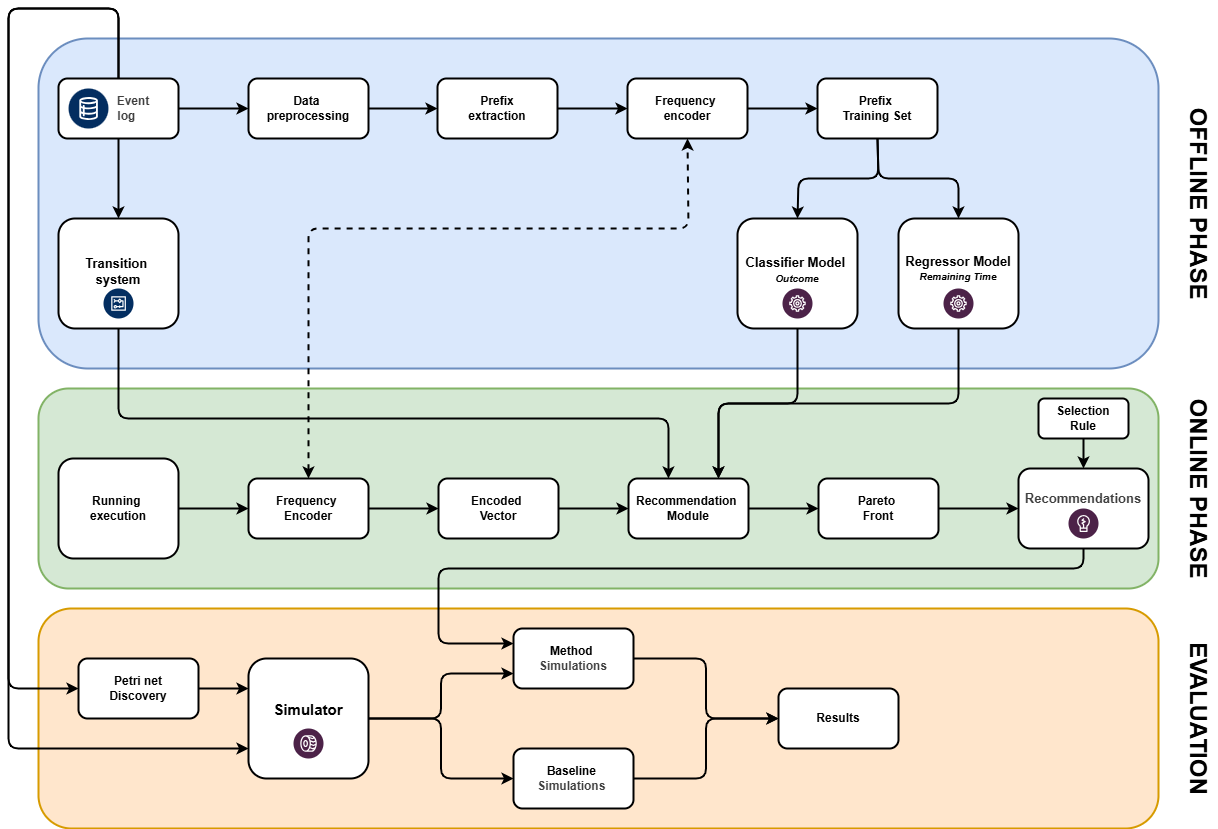
\includegraphics[width=\linewidth]{diagramma.drawio.png} \\
            \vspace{0.1cm}
            \footnotesize{(Multi-model, Pareto Front generation)}
        \end{column}
    \end{columns}
\end{frame}

\section{Offline Phase}

\begin{frame}[plain,c]
    \centering
    \color{Darkcandyapplered}
    \Huge\textbf{Offline Phase}
\end{frame}

% =====================================================================
% START-TIME ESTIMATION
% =====================================================================
\begin{frame}{Removing the \texttt{W\_} Work Items (BPI12, bpi17)}
  \small
  \begin{itemize}
    \item The BPI12 and BPI17 logs mix three kinds of events: \texttt{A\_} (application
      states), \texttt{O\_} (offer states) and \texttt{W\_} (work items of the bank's employees).
    \item All the \texttt{W\_} events are \alert{removed}: the logs keep only the
      \texttt{A\_} and \texttt{O\_} activities. Only rows are removed: the other events, their
      attributes and order, and the set of cases are unchanged (no case consists only of
      \texttt{W\_} events).
  \end{itemize}
  \begin{center}\setlength{\tabcolsep}{5pt}
  \begin{tabular}{lrrrrr}
    \toprule
    Dataset & Cases & Events before & \texttt{W\_} events removed & Events after & Activities \\
    \midrule
    BPI12        &  4\,685 & 115\,016 & 52\,902 (46.0\%) &  62\,114 & 23 $\rightarrow$ 17 \\
    bpi17-before & 12\,121 & 184\,506 & 17\,959 (9.7\%)  & 166\,547 & 24 $\rightarrow$ 18 \\
    bpi17-after  & 14\,066 & 209\,877 & 17\,154 (8.2\%)  & 192\,723 & 24 $\rightarrow$ 18 \\
    \bottomrule
  \end{tabular}
  \end{center}
  \begin{itemize}
    \item Six \texttt{W\_} activities per dataset. The filtered log is the input of the
      start-time estimation (next slide), which uses only its completion times.
  \end{itemize}
  {\scriptsize Script: \texttt{0\_filtering\_W\_activities.py} $\rightarrow$ \texttt{log\_<case>\_no\_start\_W\_filtered.xes}.}
\end{frame}

\begin{frame}{Start-Time Estimation: the Technique}
  \footnotesize
  \textbf{Problem:} in BPI12 and bpi17 the recorded start is \alert{fake} (a copy of the previous completion)
  $\Rightarrow$ waiting time always 0. BAC records real starts (untouched).\par
  {\scriptsize Vinci et al., \textit{Improving organizational processes in healthcare through
  simulation-driven resource allocation}, Artif.\ Intell.\ Med.\ 176 (2026), Appendix A ---
  extending Fracca et al.\ (CAiSE 2022).}
  \begin{itemize}
    \item One parameter $\alpha(a) \in [0,1]$ per activity $a$; the start of an event $e$ of
      activity $a$ lies between its \alert{earliest possible start} and its completion:
      \[
        t_{\text{start}}(e) = \alpha(a)\, \textit{mintime}(e) + \bigl(1-\alpha(a)\bigr)\, \textit{time}(e),
        \qquad
        \textit{mintime}(e) = \max\bigl(\textit{time}(e_{i-1}),\ \textit{time}(e^{r}_{\text{prev}})\bigr)
      \]
    \item $e_{i-1}$: previous event of the case; $e^{r}_{\text{prev}}$: previous event of the same
      resource (one activity at a time). $\alpha = 1$: as soon as possible; $\alpha = 0$: instantaneous.
  \end{itemize}
  \centering
  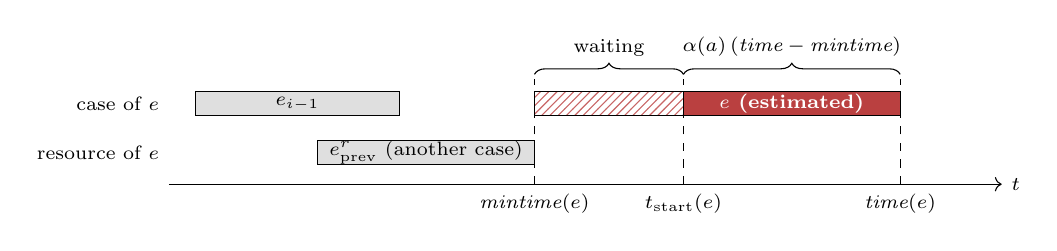
\begin{tikzpicture}[x=0.86cm,y=0.62cm,font=\scriptsize]
    \node[anchor=east] at (0,2) {case of $e$};
    \node[anchor=east] at (0,1) {resource of $e$};
    \draw[->] (0,0.35) -- (12.3,0.35) node[anchor=west] {$t$};
    \draw[fill=gray!25] (0.4,1.75) rectangle (3.4,2.25);
    \node at (1.9,2) {$e_{i-1}$};
    \draw[fill=gray!25] (2.2,0.75) rectangle (5.4,1.25);
    \node at (3.8,1) {$e^{r}_{\text{prev}}$ (another case)};
    \draw[pattern=north east lines, pattern color=Darkcandyapplered!60] (5.4,1.75) rectangle (7.6,2.25);
    \draw[fill=Darkcandyapplered!75] (7.6,1.75) rectangle (10.8,2.25);
    \node[white] at (9.2,2) {\textbf{$e$ (estimated)}};
    \draw[dashed] (5.4,0.35) -- (5.4,2.5);
    \draw[dashed] (7.6,0.35) -- (7.6,2.5);
    \draw[dashed] (10.8,0.35) -- (10.8,2.5);
    \node[below] at (5.4,0.35) {$\textit{mintime}(e)$};
    \node[below] at (7.6,0.35) {$t_{\text{start}}(e)$};
    \node[below] at (10.8,0.35) {$\textit{time}(e)$};
    \draw[decorate,decoration={brace,amplitude=4pt}] (5.4,2.6) -- (7.6,2.6)
      node[midway,above=3pt] {waiting};
    \draw[decorate,decoration={brace,amplitude=4pt}] (7.6,2.6) -- (10.8,2.6)
      node[midway,above=3pt] {$\alpha(a)\,(\textit{time} - \textit{mintime})$};
  \end{tikzpicture}
\end{frame}

% =====================================================================
% ENCODING & TRAINING INPUT
% =====================================================================
\begin{frame}{Frequency Encoder: From Traces to Feature Vectors}
    \begin{itemize}
        \item Traces have variable length, but the predictive models need a fixed-size numeric input: this is the role of the \textbf{Frequency Encoder} in the architecture diagram -- it turns a prefix of \emph{any} length into a fixed-size feature vector.
        \item \textbf{Core mechanism -- activity frequency counts:} for every activity in the log, a running counter column \texttt{\# ACTIVITY=<name>} tracks how many times that activity has already occurred in the prefix -- a bag-of-activities-style representation, independent of the prefix length.
        \item \textbf{Engineered temporal features:} time elapsed since trace start, time since the previous event, and the duration of the last completed event.
        \item \textbf{Case/event attributes:} categorical fields (activity, resource, weekday, and case-specific attributes) are one-hot encoded; continuous fields (e.g., requested amount) are standardized.
    \end{itemize}
\end{frame}

\begin{frame}{Training Input: One Row per Prefix}
  \small
  Each event $e_i$ of a training case yields one row: the \alert{state} of the case
  after $e_i$ has completed, plus the step that \alert{actually followed} it.
  \vspace{0.4cm}
  \begin{center}
  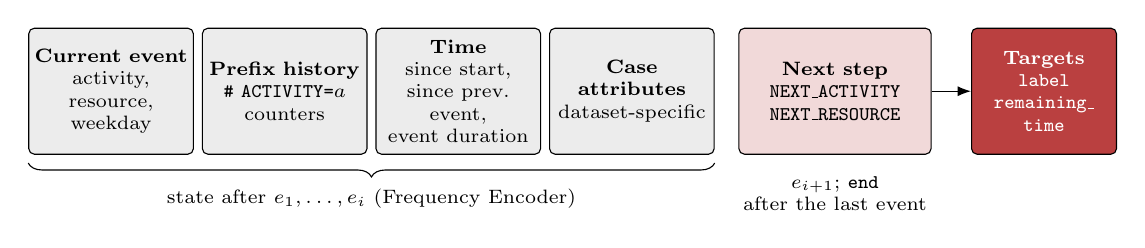
\begin{tikzpicture}[
      box/.style={draw, rounded corners=2pt, align=center, minimum height=1.6cm,
                  text width=1.95cm, font=\scriptsize, inner sep=2pt},
      node distance=0.1cm]
    \node[box, fill=gray!15] (cur) {\textbf{Current event}\\activity, resource,\\weekday};
    \node[box, fill=gray!15, right=of cur] (hist) {\textbf{Prefix history}\\\texttt{\# ACTIVITY=}$a$\\counters};
    \node[box, fill=gray!15, right=of hist] (time) {\textbf{Time}\\since start,\\since prev.\ event,\\event duration};
    \node[box, fill=gray!15, right=of time] (attr) {\textbf{Case}\\\textbf{attributes}\\dataset-specific};
    \node[box, fill=Darkcandyapplered!15, right=0.3cm of attr, text width=2.3cm] (next) {\textbf{Next step}\\\texttt{NEXT\_ACTIVITY}\\\texttt{NEXT\_RESOURCE}};
    \node[box, fill=Darkcandyapplered!75, text=white, right=0.5cm of next, text width=1.7cm] (y) {\textbf{Targets}\\\texttt{label}\\\texttt{remaining\_}\\\texttt{time}};
    \draw[-{Latex}] (next) -- (y);
    \draw[decorate,decoration={brace,amplitude=5pt,mirror}]
      ([yshift=-3pt]cur.south west) -- ([yshift=-3pt]attr.south east)
      node[midway,below=6pt,font=\scriptsize] {state after $e_1,\dots,e_i$ (Frequency Encoder)};
    \node[below=0.15cm of next, font=\scriptsize, align=center] {$e_{i+1}$; \texttt{end}\\after the last event};
  \end{tikzpicture}
  \end{center}
\end{frame}

\begin{frame}{Training Input: Next Step and Targets}
  \begin{itemize}
    \item \textbf{Why the next step is an input:} at recommendation time
      \texttt{NEXT\_ACTIVITY} / \texttt{NEXT\_RESOURCE} are replaced by each candidate
      \texttt{(activity, resource)} pair, so the models answer
      ``what happens if the case continues \emph{with this step}?''.
    \item \textbf{Targets}:
      \begin{itemize}
        \item \texttt{label}: case outcome (1 $=$ positive, defined per dataset),
          the same for all rows of a case $\rightarrow$ classifier;
        \item \texttt{remaining\_time}: time from the completion of $e_i$ to the end of the case, in
          seconds $\rightarrow$ regressor (learned as $\log(1+\text{days})$, see the time-target slides).
      \end{itemize}
    \item Case id and timestamps are not model inputs.
  \end{itemize}
\end{frame}

\begin{frame}{Training Input: an Example Row (BPI12)}
  \small
  Case \texttt{173721}, 9th event (current training set).
  \begin{center}
  \scriptsize
  \begin{tabular}{lll}
    \toprule
    \textbf{Column} & \textbf{Value} & \textbf{Meaning} \\
    \midrule
    \texttt{concept:name}      & \texttt{O\_SENT\_BACK} & activity just completed \\
    \texttt{org:resource}      & \texttt{11029}  & who executed it \\
    \texttt{weekday}           & Saturday        & day of its start \\
    \texttt{AMOUNT\_REQ}       & 9000            & requested amount (case attr.) \\
    \texttt{\# ACTIVITY=A\_SUBMITTED}, \dots & 1 (8 counters), 0 (9) & activities before $e_i$ \\
    \texttt{time\_from\_start} & 794.8\,s & start($e_i$) - start($e_1$) \\
    \texttt{time\_from\_previous\_event(start)} & 0.02\,s & start($e_i$) - start($e_{i-1}$) \\
    \texttt{event\_duration}   & 4.94\,d & end($e_i$)  - start($e_i$) (estimated start) \\
    \midrule
    \texttt{NEXT\_ACTIVITY} / \texttt{NEXT\_RESOURCE} & \texttt{A\_DECLINED} / \texttt{11009} & step that followed \\
    \midrule
    \texttt{label}            & 0     & \texttt{O\_ACCEPTED} never occurs \\
    \texttt{remaining\_time}  & 369\,519\,s $=$ 4.28 d & regression target \\
     & $\log(1 + 4.28) = 1.66$ & what the regressor learns \\
    \bottomrule
  \end{tabular}
  \end{center}
\end{frame}

\begin{frame}{The ``No Recommendation'' Baseline: What Changed}
  \small
  Reference for a candidate on prefix $e_1,\dots,e_k$: \alert{what if we recommend
  nothing?}
  \vspace{0.1cm}
  \begin{columns}[T]
    \begin{column}{0.49\textwidth}
      \begin{block}{Before}
        \scriptsize
        The prefix \emph{one step shorter} $e_1,\dots,e_{k-1}$, with its real next
        step $e_k$ (a transition already observed).
        \begin{itemize}\scriptsize
          \item \alert{different state} from the candidates: the difference mixes the
            suggestion with the progress of the case (the remaining time still
            includes $e_k$);
          \item not ``nothing'', but a step that already happened;
          \item missing for single-event prefixes.
        \end{itemize}
      \end{block}
    \end{column}
    \begin{column}{0.49\textwidth}
      \begin{block}{Now}
        \scriptsize
        The \emph{same} query instance $e_1,\dots,e_k$ with \texttt{NEXT\_ACTIVITY}
        $=$ \texttt{NEXT\_RESOURCE} $=$ \texttt{\_\_NO\_NEXT\_\_}.
        \begin{itemize}\scriptsize
          \item models trained on a \alert{doubled dataset}: \texttt{\_\_NO\_NEXT\_\_}
            is a value they have learned;
          \item candidate and baseline differ \alert{only in the next step}: a true
            ``suggestion vs.\ nothing'' comparison;
          \item available for every prefix, including single-event ones.
        \end{itemize}
      \end{block}
    \end{column}
  \end{columns}
\end{frame}

\begin{frame}{Training Input: the Doubled Dataset}
  \small
  Every training row is kept \alert{and} copied with the next step blanked out;
  all other features and both targets are unchanged.
  \begin{center}
  \scriptsize
  \begin{tabular}{llllcc}
    \toprule
     & \textbf{State} $e_1,\dots,e_i$ & \texttt{NEXT\_ACTIVITY} & \texttt{NEXT\_RESOURCE} & \texttt{label} & \texttt{remaining\_time} \\
    \midrule
    original & BPI12 case \texttt{173721}, $i=9$ & \texttt{A\_DECLINED} & \texttt{11009} & 0 & 4.28 d \\
    copy     & (identical)                      & \texttt{\_\_NO\_NEXT\_\_} & \texttt{\_\_NO\_NEXT\_\_} & 0 & 4.28 d \\
    \bottomrule
  \end{tabular}
  \end{center}
  \footnotesize
  \begin{itemize}
    \item \textbf{Original rows} teach $\mathbb{E}[\,y \mid \text{state},\ \text{next step}\,]$:
      the effect of a specific \texttt{(activity, resource)} $\rightarrow$ scores the
      \emph{candidates}.
    \item \textbf{Copies} teach $\mathbb{E}[\,y \mid \text{state}\,]$: the targets from
      the state alone, averaged over what historically followed similar states
      $\rightarrow$ the \emph{baseline}.
  \end{itemize}
\end{frame}



\begin{frame}{Training Input: BAC}
  \footnotesize
  \textbf{Process:} closure of bank accounts (request, authorisation, pending
  checks, completion). 15 activities, 654 resources.
  \begin{center}
  \begin{tabular}{lp{9.2cm}}
    \toprule
    \textbf{Column} & \textbf{Meaning} \\
    \midrule
    \texttt{CLOSURE\_TYPE} (4 values) & kind of closure: Inheritance, Client Recess, Bank Recess, Porting \\
    \texttt{CLOSURE\_REASON} (9 values) & why the account is closed (e.g.\ ``Client lost'', ``Keep bank account. Same dip'') \\
    \texttt{org:role} (3 values) & role of the executing resource: APPLICANT, DIRECTOR, BACK-OFFICE \\
    15 \texttt{\# ACTIVITY} counters & e.g.\ \texttt{\# ACTIVITY=Authorization Requested} \\
    \midrule
    \texttt{label} $=1$ & the case contains \emph{neither} ``Back-Office Adjustment Requested''
      \emph{nor} ``Network Adjustment Requested'' (no rework) \\
    \bottomrule
  \end{tabular}
  \end{center}
  \begin{itemize}
    \item The two adjustment activities define the outcome $\Rightarrow$
      \alert{forbidden} as recommendations.
    \item Only dataset with real start times; shortest cases (median 7 events).
  \end{itemize}
\end{frame}

\begin{frame}{Training Input: BPI12}
  \footnotesize
  \textbf{Process:} loan applications of a Dutch bank (BPIC 2012). 17 activities,
  60 resources; the \texttt{W\_} work items are removed (offline phase).
  \begin{center}
  \begin{tabular}{lp{9.2cm}}
    \toprule
    \textbf{Column} & \textbf{Meaning} \\
    \midrule
    \texttt{AMOUNT\_REQ} (continuous) & loan amount requested by the customer \\
    \texttt{A\_} counters & application state changes (e.g.\ \texttt{A\_SUBMITTED}, \texttt{A\_PREACCEPTED}) \\
    \texttt{O\_} counters & offer state changes (e.g.\ \texttt{O\_CREATED}, \texttt{O\_SENT}) \\
    \midrule
    \texttt{label} $=1$ & an offer is accepted: \texttt{O\_ACCEPTED} occurs in the case \\
    \bottomrule
  \end{tabular}
  \end{center}
  \begin{itemize}
    \item \texttt{O\_ACCEPTED} is \alert{forbidden} as a recommendation.
    \item Most balanced outcome ($47.9\%$ positive), median 13 events per case,
      no categorical case attributes.
  \end{itemize}
\end{frame}

\begin{frame}{Training Input: bpi17-before \& bpi17-after}
  \footnotesize
  \textbf{Process:} loan applications of the same bank (BPIC 2017), two sub-logs with
  their own models. 18 activities, 103 / 119 resources; the \texttt{W\_} work items are removed.
  \begin{center}
  \begin{tabular}{lp{8.5cm}}
    \toprule
    \textbf{Column} & \textbf{Meaning} \\
    \midrule
    \texttt{RequestedAmount} (continuous) & loan amount requested \\
    \texttt{LoanGoal} (13 / 14 values) & purpose of the loan (Car, Home improvement, \dots) \\
    \texttt{ApplicationType} (2 values) & New credit / Limit raise \\
    \texttt{EventOrigin} (2 values) & object the event refers to: Application, Offer \\
    \texttt{Action} (2 values) & Created, statechange \\
    18 \texttt{\# ACTIVITY} counters & \texttt{A\_} and \texttt{O\_} activities, as in BPI12 \\
    \midrule
    \texttt{label} $=1$ & \texttt{O\_Accepted} occurs in the case \\
    \bottomrule
  \end{tabular}
  \end{center}
  \begin{itemize}
    \item Same columns in both sub-logs (in bpi17-after with the \texttt{case:}
      prefix, e.g.\ \texttt{case:LoanGoal}); \texttt{O\_Accepted} is
      \alert{forbidden} as a recommendation.
  \end{itemize}
\end{frame}

\begin{frame}{Predictive Modeling Strategy}
    \begin{itemize}
        \item The framework leverages independent Machine Learning models tailored to the specific nature of each KPI.
        \item \textbf{Implementation Example:}
        \begin{itemize}
            \item \textbf{CatBoost Regressor:} Used to predict continuous KPIs (e.g., Remaining Execution Time).
            \item \textbf{CatBoost Classifier:} Used to predict discrete or binary KPIs (e.g., Case Outcome probability via \texttt{predict\_proba}).
        \end{itemize}
        \item This decoupling provides higher accuracy and prevents conflicting objectives from diluting a single model's predictive performance.
        \item Both models are trained once, offline, on the encoded prefix training set, and reused for every case and every candidate (activity, resource) pair during the online recommendation phase.
    \end{itemize}
\end{frame}

\begin{frame}{Predictive Uncertainty Quantification}
  \begin{itemize}
    \item A point prediction (a probability, a duration) gives no indication of
      how far it can be trusted.
    \item Two sources of error, estimated separately:
      \begin{itemize}
        \item \alert{Aleatoric} (data) uncertainty: irreducible noise of the
          process; does not shrink with more data.
        \item \alert{Epistemic} (knowledge) uncertainty: the model's ignorance
          on rare or unseen \texttt{(activity, resource)} inputs; shrinks with
          more data, flags out-of-domain candidates.
      \end{itemize}
    \item \textbf{Both} CatBoost models now report this decomposition --- for the
      outcome classifier and the remaining-time regressor.
    \item Online, the per-member predictions are used to estimate the
      \alert{probability that a candidate beats the no-recommendation baseline}
      (confidence filter).
  \end{itemize}

\end{frame}

\begin{frame}{Error decomposition}
    \begin{figure}\centering
        \includegraphics[width=0.78\linewidth]{aleatoric_epistemic.png}
    \end{figure}
\end{frame}

\begin{frame}{Estimating Uncertainty: SGLB \& Virtual Ensembles}
  \begin{itemize}
    \item Both models are trained with \alert{Stochastic Gradient Langevin
      Boosting} (\texttt{posterior\_sampling=True}): Gaussian noise injected in
      the gradient makes the training asymptotically sample the parameter
      posterior $p(\theta \mid \mathcal{D})$.
    \item At inference a \alert{virtual ensemble} is read from the single trained
      model, using truncations of its tree sequence --- an ensemble at the cost
      of one model.
    \item \textbf{Regressor} (\texttt{RMSEWithUncertainty}, in the space it learns), law of total
      variance:
      \[
        \underbrace{\sigma_{\text{tot}}^{2}}_{\text{total}} =
        \underbrace{\operatorname{Var}_{m}[\mu_{m}]}_{\text{knowledge}} +
        \underbrace{\tfrac{1}{M}\textstyle\sum_{m}\sigma_{m}^{2}}_{\text{data}}
      \]
    \item \textbf{Classifier}: entropy decomposition: total entropy $=$
      expected member entropy (data) $+$ mutual information (knowledge).
  \end{itemize}
\end{frame}

\begin{frame}{Calibration of the Predictive Models}
  A reported probability or interval is only useful if it matches reality, and
  boosted models tend to be \alert{overconfident}. Each fix is one scalar,
  fitted on a held-out slice, applied to the frozen model.
  \begin{itemize}
    \item \textbf{Classifier $ \rightarrow$ temperature scaling:}
      $p_{\text{cal}} = \sigma\!\left(\sigma^{-1}(p)/T\right)$, $T$ minimising
      log-loss. Monotone $\Rightarrow$ predicted label unchanged, only the
      probability is rescaled. Diagnostic: ECE, before vs after.
    \item \textbf{Regressor $ \rightarrow$ $\sigma$-scaling:} every predicted $\sigma$ (in the space the
      model learns) is multiplied by $s$, minimising the Gaussian NLL; closed form
      $s = \bigl(\tfrac{1}{L}\sum_{j}(y_{j}-\hat y_{j})^{2}/\sigma_{j}^{2}\bigr)^{1/2}$.
      Diagnostics: ENCE and $\pm1\sigma$ / $\pm2\sigma$ coverage
      (target $68\%$ / $95\%$).
  \end{itemize}
\end{frame}

\begin{frame}{Remaining-Time Target: Four Candidates}
  \scriptsize
  Time regressor trained as in step 2 (Optuna 80 trials, \texttt{RMSEWithUncertainty}, $\sigma$-scaling); only the
  space it learns in changes. Predictions back in seconds (log spaces: plain log-normal \alert{mean});
  errors in \alert{days}.
  \begin{center}\tiny\setlength{\tabcolsep}{4pt}\setlength{\aboverulesep}{0pt}\setlength{\belowrulesep}{1pt}
  \begin{tabular}{lcccc}
    \toprule
    Test MAE / RMSE (d) & \texttt{sigmoid\_mm}$^{*}$ & seconds (\texttt{none}) & $\log(1+\text{seconds})$ & $\log(1+\text{days})$ \\
    \midrule
    BAC          & 4.94 / 18.39 & 5.65 / 18.23 & 5.61 / \alert{44.94}   & 5.10 / 18.05 \\
    BPI12        & 8.29 / 12.47 & 7.82 / 11.96 & 8.47 / 15.47           & 7.86 / 11.94 \\
    bpi17-before & 9.62 / 14.34 & 9.32 / 13.80 & 9.11 / 13.20           & \alert{15.91 / 684.3} \\
    bpi17-after  & 8.84 / 13.54 & 8.77 / 13.38 & \alert{22.86 / 1651}   & 8.31 / 12.79 \\
    \midrule
    ENCE / cov.\ $\pm2\sigma$ (\%) & & & & \\
    \midrule
    BAC          & 35.4 / 96.0 & 36.0 / 98.5 & 21.9 / 97.9 & 28.4 / 97.8 \\
    BPI12        & 15.1 / 94.6 & 28.4 / 93.8 & 14.9 / 97.1 & 14.1 / 95.8 \\
    bpi17-before & 27.7 / 95.3 & 32.1 / 91.9 & 19.1 / 98.8 & 13.7 / 95.7 \\
    bpi17-after  & 23.6 / 94.6 & 43.3 / 90.4 & 25.0 / 98.5 & 17.3 / 97.6 \\
    \bottomrule
  \end{tabular}
  \end{center}
  \vspace{-0.2cm}
  \begin{itemize}
    \item Log spaces: best uncertainty (lower ENCE, coverage target 95.4\%), but the mean \alert{explodes} on a
      few test cases (red, next slide). Seconds: stable mean, worst calibration.
  \end{itemize}
  {\tiny $^{*}$Models of 2026-10-07: same data only for BAC; BPI12/bpi17 then still had the \texttt{W\_}
  activities and the previous start times (indicative). Source: \texttt{2b\_time\_target\_comparison.txt}.}
\end{frame}

\begin{frame}{Log-Space Target: Back to Days}
  \scriptsize
  The model learns $X = \log(1 + T/\text{86\,400})$, $T$ the remaining time in seconds, and predicts
  $X \sim \mathcal{N}(\mu, \sigma^2)$ per prefix: $T = \text{86\,400}\,(e^X - 1)$ is \alert{log-normal}.
  \begin{itemize}
    \item \textbf{Naive inverse} $e^{\mu}-1$: $e^x$ is monotone, so it maps the median of $X$ to the
      \alert{median} of $T$ ($P(X \le \mu) = 1/2$), not to its mean.
    \item \textbf{Mean} (what the recommender minimises): integrate $e^x$ against the Gaussian density
      \[
        \mathbb{E}[e^X] = \int_{-\infty}^{+\infty} e^{x}\,\frac{1}{\sigma\sqrt{2\pi}}\,
          e^{-\frac{(x-\mu)^2}{2\sigma^2}}\,dx,
        \qquad
        x - \frac{(x-\mu)^2}{2\sigma^2} = -\frac{\bigl(x-(\mu+\sigma^2)\bigr)^2}{2\sigma^2} + \mu + \frac{\sigma^2}{2}
      \]
      (completing the square). The first term is the exponent of a Gaussian $\mathcal{N}(\mu+\sigma^2,\sigma^2)$,
      whose density integrates to 1:
      \[
        \mathbb{E}[e^X] = e^{\mu + \sigma^2/2}\int_{-\infty}^{+\infty}\mathcal{N}(x;\,\mu+\sigma^2,\sigma^2)\,dx
          = e^{\mu}\cdot e^{\sigma^2/2},
        \qquad
        \mathbb{E}[T] = \text{86\,400}\bigl(e^{\mu}e^{\sigma^2/2} - 1\bigr)
      \]
    \item The mean is the median scaled by $e^{\sigma^2/2} \ge 1$ (on $1 + T/\text{86\,400}$): $e^x$ is convex,
      so the naive inverse underestimates the expected time (Jensen), most where $\sigma$ is large.
    \item \textbf{Why it explodes:} $\sigma^2$ is in the exponent. Typical prefix $\sigma^2 \approx 0.4$, factor
      $e^{0.2} \approx 1.2$. A prefix with two very different outcomes (\texttt{A\_Incomplete}: closed now or
      cancelled after $\sim$30 d) is bimodal in log space; a single Gaussian covers both modes with
      $\sigma^2 \approx 13$, factor $\approx 840$: \alert{2142 d} predicted (true 15.9, longest case 135).
  \end{itemize}
\end{frame}

\begin{frame}{Log-Space Target: the Truncated Log-Normal}
  \scriptsize\setlength{\abovedisplayskip}{2pt}\setlength{\belowdisplayskip}{2pt}
  No remaining time can exceed the longest one of the training set, $U$: we use the distribution of $T$
  \alert{given $T \le U$}, i.e.\ $X \le u$ with $u = \log(1 + U/\text{86\,400})$.
  \begin{enumerate}
    \item \textbf{Condition on $X \le u$:} integrate the density $f$ only up to $u$, divide by
      $P(X \le u) = \Phi\bigl(\frac{u-\mu}{\sigma}\bigr)$:
      \[
        \mathbb{E}[e^X \mid X \le u] = \frac{1}{\Phi\bigl(\frac{u-\mu}{\sigma}\bigr)}\int_{-\infty}^{u} e^{x}\, f(x)\,dx
      \]
    \item \textbf{Same completed square}, but the integral now stops at $u$, so it is the CDF of
      $\mathcal{N}(\mu+\sigma^2,\sigma^2)$ at $u$:\;
      $\int_{-\infty}^{u} e^{x} f(x)\,dx = e^{\mu + \sigma^2/2}\,\Phi\bigl(\frac{u - \mu - \sigma^2}{\sigma}\bigr)$.
  \end{enumerate}
  \begin{block}{Correction: log-normal truncated at $U$}
    \centering
    $\mathbb{E}[T \mid T \le U] = \text{86\,400}\Bigl(e^{\mu + \sigma^2/2}\,
      \Phi\bigl(\tfrac{u - \mu - \sigma^2}{\sigma}\bigr) \big/ \Phi\bigl(\tfrac{u - \mu}{\sigma}\bigr) - 1\Bigr)$
  \end{block}
  \begin{itemize}
    \item \textbf{Typical prefix:} $u$ far above $\mu + \sigma^2$, both $\Phi \approx 1$ $\Rightarrow$ the plain mean
      (17.6 d $\rightarrow$ 17.6 d). \textbf{Large $\sigma^2$:} $(u-\mu-\sigma^2)/\sigma$ very negative, the
      $\Phi$ in the numerator cancels $e^{\sigma^2/2}$ (2142 d $\rightarrow$ \alert{11.1 d}). Never above $U$.
    \item Same for the median, $\mu + \sigma\,\Phi^{-1}\bigl(\Phi(\frac{u-\mu}{\sigma})/2\bigr)$, and the std
      (via $\mathbb{E}[e^{2X} \mid X \le u]$); checked by Monte Carlo. The confidence filter is unchanged
      ($P(A<B)$ in log space). Post-hoc: the model is fitted untruncated; $U$ exceeded by 47 of 26\,095 test
      rows (bpi17-after).
  \end{itemize}
\end{frame}

\begin{frame}{Log-Space Target: With and Without the Truncation}
  \scriptsize
  Same saved models, only the transformation back to days changes. $>U$: test predictions longer than the
  longest remaining time of the training set (largest prediction in brackets).
  \begin{center}\tiny\setlength{\tabcolsep}{3.5pt}\setlength{\aboverulesep}{0pt}\setlength{\belowrulesep}{1pt}
  \begin{tabular}{lccccc}
    \toprule
     & seconds & \multicolumn{2}{c}{$\log(1+\text{days})$} & \multicolumn{2}{c}{$\log(1+\text{seconds})$} \\
    \cmidrule(lr){3-4}\cmidrule(lr){5-6}
    Test MAE / RMSE (d) & (\texttt{none}) & plain & \alert{truncated} & plain & \alert{truncated} \\
    \midrule
    BAC ($U$ = 504 d)          & 5.65 / 18.23 & 5.10 / 18.05    & \textbf{5.09 / 18.05} & 5.61 / 44.94  & 5.19 / 18.03 \\
    BPI12 ($U$ = 91 d)         & \textbf{7.82 / 11.96} & 7.86 / 11.94 & 7.91 / 12.03 & 8.47 / 15.47 & 8.05 / 12.20 \\
    bpi17-before ($U$ = 136 d) & 9.32 / 13.80 & 15.91 / 684.3   & 9.15 / 13.67          & 9.11 / 13.20  & \textbf{8.96 / 13.16} \\
    bpi17-after ($U$ = 101 d)  & 8.77 / 13.38 & 8.31 / 12.79    & 8.42 / 12.96          & 22.86 / 1651  & 8.47 / 12.88 \\
    \midrule
    Predictions $> U$ & & & & & \\
    \midrule
    BAC          & 0 & 0 (39)     & 0 (33) & 1 (4\,910)     & 0 (47) \\
    BPI12        & 0 & 0 (31)     & 0 (27) & 9 (603)        & 0 (24) \\
    bpi17-before & 0 & 19 (89\,029) & 0 (40) & 1 (142)      & 0 (38) \\
    bpi17-after  & 0 & 0 (34)     & 0 (34) & 31 (255\,225)  & 0 (29) \\
    \bottomrule
  \end{tabular}
  \end{center}
  \vspace{-0.2cm}
  \begin{itemize}
    \item The truncation removes every absurd prediction and leaves the well-behaved cases unchanged.
      Truncated log spaces beat seconds on BAC and bpi17 (MAE $-$0.3 to $-$0.6 d), BPI12 $+$0.09 d.
    \item Chosen: \alert{$\log(1+\text{days})$ truncated}: needs the truncation least (absurd predictions on one
      dataset, not three) and has the best calibration.
  \end{itemize}
\end{frame}

\begin{frame}{Predictive Models: Fit on Train and Test}
  \small
  Classifier: Logloss. Regressor: $\log(1+\text{days})$ with the truncated log-normal mean, errors in
  \alert{days}. Train: the doubled training set (with the no-recommendation copies).
  \begin{center}\setlength{\tabcolsep}{5pt}
  \begin{tabular}{lcccccc}
    \toprule
     & \multicolumn{2}{c}{Outcome classifier} & \multicolumn{4}{c}{Remaining-time regressor} \\
    \cmidrule(lr){2-3}\cmidrule(lr){4-7}
     & \multicolumn{2}{c}{Logloss} & \multicolumn{2}{c}{RMSE (d)} & \multicolumn{2}{c}{MAE (d)} \\
    \cmidrule(lr){2-3}\cmidrule(lr){4-5}\cmidrule(lr){6-7}
    Dataset & train & test & train & test & train & test \\
    \midrule
    BAC          & 0.192 & 0.214 & 17.65 & 18.05 & 4.70 & 5.09 \\
    BPI12        & 0.469 & 0.494 &  9.05 & 12.03 & 5.99 & 7.91 \\
    bpi17-before & 0.469 & 0.482 &  9.76 & 13.67 & 6.93 & 9.15 \\
    bpi17-after  & 0.479 & 0.477 &  9.42 & 12.96 & 6.88 & 8.42 \\
    \bottomrule
  \end{tabular}
  \end{center}
  \footnotesize
  \begin{itemize}
    \item Test: every prefix of the test cases. Classifier: test Logloss at most $0.025$ above train (none on
      bpi17-after). Regressor: test MAE above train by $1.5$--$2.2$ d on BPI12 and bpi17, $0.4$ d on BAC.
  \end{itemize}
\end{frame}

\begin{frame}{Predictive Models: Uncertainty \& Calibration}
  \footnotesize
  Test set. Arrows: raw $\rightarrow$ calibrated. ECE / ENCE in \%. Regressor diagnostics in the space it
  learns, $\log(1+\text{days})$: a $\pm k\sigma$ interval there is the same quantile interval in days.
  \begin{center}\setlength{\tabcolsep}{4pt}
  \begin{tabular}{lcccccc}
    \toprule
     & \multicolumn{2}{c}{Classifier} & \multicolumn{4}{c}{Regressor} \\
    \cmidrule(lr){2-3}\cmidrule(lr){4-7}
    Dataset & ECE & $T$ & ENCE & $s$ & cov.\ $\pm1\sigma$ & cov.\ $\pm2\sigma$ \\
    \midrule
    BAC          & $2.5 \rightarrow$ \textbf{2.0} & 1.057 & $27.1 \rightarrow 28.4$          & 1.039 & $86.5 \rightarrow 87.8$ & $97.6 \rightarrow 97.8$ \\
    BPI12        & $7.0 \rightarrow 7.0$          & 0.933 & $20.1 \rightarrow$ \textbf{14.1} & 1.075 & $59.4 \rightarrow 63.7$ & $94.8 \rightarrow 95.8$ \\
    bpi17-before & $8.4 \rightarrow 8.5$          & 0.959 & $13.4 \rightarrow 13.7$          & 0.997 & $58.9 \rightarrow 58.7$ & $95.8 \rightarrow 95.7$ \\
    bpi17-after  & $4.2 \rightarrow$ \textbf{3.8} & 1.091 & $16.6 \rightarrow 17.3$          & 1.053 & $70.8 \rightarrow 74.1$ & $96.6 \rightarrow 97.6$ \\
    \bottomrule
  \end{tabular}
  \end{center}
  \vspace{-0.2cm}
  \scriptsize
  \begin{itemize}
    \item \alert{Epistemic} uncertainty negligible ($\le 0.1\%$ of the classifier's entropy, $\le 0.2\%$ of the
      regressor's variance): kept only as an out-of-domain flag.
    \item \textbf{Classifier:} $T = 0.93$--$1.09$, already close to calibrated; temperature scaling lowers ECE on
      BAC and bpi17-after and leaves it unchanged on BPI12 and bpi17-before ($T$ is fitted on a held-out slice).
    \item \textbf{Regressor:} $s \approx 1$; $\pm2\sigma$ covers $95.7$--$97.8\%$ (target $95.4\%$). $\sigma$-scaling
      lowers ENCE only on BPI12; elsewhere $< 1.3$ points ($s$ minimises the NLL, not the ENCE). $\pm1\sigma$
      above $68\%$ on BAC, below on BPI12 and bpi17-before: residuals more peaked and heavier-tailed than a
      Gaussian.
  \end{itemize}
\end{frame}

\section{Online Phase}

\begin{frame}[plain,c]
    \centering
    \color{Darkcandyapplered}
    \Huge\textbf{Online Phase}
\end{frame}

\begin{frame}{Recommendation Generation}
  \small
  \begin{itemize}
    \item For a running case, the feasibility module returns the valid
      \texttt{(activity, resource)} candidates: the next activities that followed the same window (last 5
      activities) in at least 1\% of the training cases, each with the resources that executed it after that
      window in at least 5\% of the cases (the most frequent one always kept) --- on average
      $3\text{--}14$ per prefix, depending on the dataset.
    \item Each candidate is scored by the two models, by placing it in the
      \texttt{NEXT\_ACTIVITY} / \texttt{NEXT\_RESOURCE} columns of the query instance.
    \item \alert{Confidence filter:} a candidate is kept only if it is likely enough
      to beat the \emph{no-recommendation} baseline on at least one KPI (next slides).
    \item The survivors are compared on \alert{two objectives}, optimised jointly:
      \begin{itemize}
        \item outcome probability (maximised);
        \item expected remaining time in days (minimised).
      \end{itemize}
    \item The \alert{non-dominated} candidates form the Pareto front.
    \item Exhaustive evaluation: a single vectorised pass over all feasible pairs — exact and, at this scale, fast.
  \end{itemize}
\end{frame}

% =====================================================================
% CONFIDENCE FILTER
% =====================================================================
\begin{frame}{Confidence Filter: Motivation}
  \small
  \begin{itemize}
    \item The Pareto front compares candidates \emph{only with each other}. A
      non-dominated candidate can still be:
      \begin{itemize}
        \item predicted \alert{worse than not intervening} at all;
        \item better only by a margin far \alert{below the model's own uncertainty}.
      \end{itemize}
    \item Earlier version: the predictive standard deviation of the time was a
      \emph{third Pareto objective}. But $\sigma$ alone says how noisy a prediction
      is, not whether the candidate improves on anything, and a noisy candidate
      could still enter the front through the other two axes.
    \item \textbf{New question}, asked for each candidate and each KPI:
      \begin{block}{}
        \centering
        How likely is it that following this candidate is \emph{better} than giving
        no recommendation?
      \end{block}
    \item One number per KPI that combines \alert{effect size} (difference of the
      predictions) and \alert{uncertainty}, readable as a probability
      $\Rightarrow$ a threshold $\gamma$ has a direct meaning.
  \end{itemize}
\end{frame}

\begin{frame}{Confidence Filter: the Baseline}
  \small
  \begin{itemize}
    \item \textbf{Baseline} $B$: the query instance of the case with
      \texttt{NEXT\_ACTIVITY} $=$ \texttt{NEXT\_RESOURCE} $=$ \texttt{\_\_NO\_NEXT\_\_}
      --- the value learned from the doubled training set (offline phase).
    \item It predicts outcome and remaining time from \emph{the same state} as the
      candidates, when the process continues as it historically did.
    \item \textbf{Candidate} $A$: the same query instance with the candidate
      \texttt{(activity, resource)} as next step.
    \item Both are scored by \alert{every member} $m = 1,\dots,M$ of the same
      virtual ensemble ($M \le 50$):
      \begin{itemize}
        \item \textbf{outcome}: calibrated \alert{logit} $a_m, b_m$ --- unbounded,
          so a Gaussian model is sensible (the probability is bounded in $[0,1]$);
          the logit is monotone in the probability, so $P(\text{logit}_A >
          \text{logit}_B) = P(p_A > p_B)$;
        \item \textbf{time}: predicted mean $a_m, b_m$ in the space the regressor learns, $\log(1+\text{days})$, plus each member's own (aleatoric) variance $\sigma^2_{A,m}$, $\sigma^2_{B,m}$; the resulting std is multiplied by the $\sigma$-scaling factor $s$ (calibrated).

      \end{itemize}
  \end{itemize}
\end{frame}

\begin{frame}{Confidence Filter: Probability of Beating the Baseline}
  \footnotesize
  $A$ and $B$ modelled as \alert{correlated Gaussians}, with moments estimated from
  the $M$ paired members:
  \[
    \bar d = \bar a - \bar b, \qquad
    s_d^{2} = s_A^{2} + s_B^{2} - 2\, s_{AB}, \qquad
    s_{AB} = \tfrac{1}{M-1}\textstyle\sum_{m}(a_m-\bar a)(b_m-\bar b)
  \]
  \begin{itemize}
    \item \textbf{time}: predicted mean $a_m, b_m$ in the space the regressor learns, $\log(1+\text{days})$, plus each member's own (aleatoric) variance $\sigma^2_{A,m}$, $\sigma^2_{B,m}$; the resulting std is multiplied by the $\sigma$-scaling factor $s$ (calibrated). Monotone way back to days: same $P(\text{time}_A < \text{time}_B)$.

    \item Posterior predictive of a new difference (normal population, unknown mean
      and variance): $D \sim t_{M-1}\bigl(\bar d,\ s_d^2 (1 + 1/M)\bigr)$, hence
  \end{itemize}
  \[
    P(A > B) = T_{M-1}\!\left(\frac{\bar d}{s_d\sqrt{1 + 1/M}}\right)
  \]
  \vspace{-0.2cm}
  \[
    p_{\text{out}} = P(\text{outcome}_A > \text{outcome}_B), \qquad
    p_{\text{time}} = 1 - P(\text{time}_A > \text{time}_B) \quad \text{(shorter is better)}
  \]
\end{frame}

\begin{frame}{Confidence Filter: Modelling Choices}
  \begin{itemize}
    \item \textbf{Why paired:} member $m$ scores both $A$ and $B$, so their errors are
      positively correlated; assuming independence would overstate $s_d$ and push
      every probability towards $0.5$.
    \item \textbf{Why Student-$t$ and not the normal CDF:} mean and variance are
      \emph{estimated} from only $M$ members; the $t$ distribution with $M-1$ degrees
      of freedom and the $(1+1/M)$ factor account for it, and tend to the plain
      $z$-test as $M \to \infty$.
    \item \textbf{Why the logit for the outcome:} a probability lives in $[0,1]$ and is
      poorly described by a Gaussian; the logit is unbounded and monotone in it.
    \item \textbf{Why only the time uses the aleatoric part:} for the time we compare the remaining times the case may actually take, so each member's own variance $\sigma_m^2$ is part of the prediction. For the outcome we compare the \emph{probabilities} of success: the aleatoric noise of a classifier is the $0/1$ result of the single case, $p_m(1-p_m)$, not uncertainty about $p$ itself, so it does not enter the comparison.

  \end{itemize}
\end{frame}

\begin{frame}{Confidence Filter: the Rule}
  \begin{block}{}
    \centering
    keep candidate $\iff$ $p_{\text{out}} > \gamma_{\text{cls}}$ \ \textbf{or} \
    $p_{\text{time}} > \gamma_{\text{reg}}$ \qquad (default $\gamma_{\text{cls}} = \gamma_{\text{reg}} = 0.5$)
  \end{block}
  \vspace{0.1cm}
  \centering
  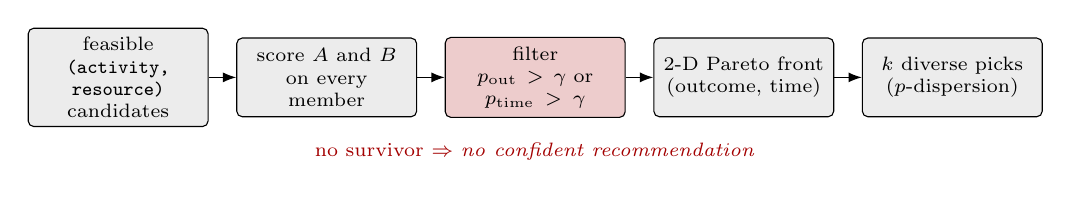
\begin{tikzpicture}[
      stage/.style={draw, rounded corners=2pt, align=center, font=\scriptsize,
                   text width=2.05cm, minimum height=1.0cm, fill=gray!15},
      node distance=0.35cm]
    \node[stage] (c) {feasible\\\texttt{(activity, resource)}\\candidates};
    \node[stage, right=of c] (s) {score $A$ and $B$\\on every member};
    \node[stage, fill=Darkcandyapplered!20, right=of s] (f) {filter\\$p_{\text{out}} > \gamma$ or\\$p_{\text{time}} > \gamma$};
    \node[stage, right=of f] (p) {2-D Pareto front\\(outcome, time)};
    \node[stage, right=of p] (k) {$k$ diverse picks\\($p$-dispersion)};
    \draw[-{Latex}] (c) -- (s); \draw[-{Latex}] (s) -- (f);
    \draw[-{Latex}] (f) -- (p); \draw[-{Latex}] (p) -- (k);
    \node[below=0.2cm of f, font=\scriptsize, align=center, text=Darkcandyapplered]
      {no survivor $\Rightarrow$ \emph{no confident recommendation}};
  \end{tikzpicture}
  \footnotesize
  \begin{itemize}
    \item Uncertainty is no longer a Pareto axis: it acts as a \alert{gate} before the
      front, which is built on the two KPIs only.
    \item If nothing survives, the case receives \emph{no} recommendation rather than a
      doubtful one: letting the process continue is itself the safe choice.
    \item A candidate passes if it is likely enough to improve \alert{at least one} KPI;
      it may be predicted worse on the other one, and the trade-off is left to the
      Pareto front. Raising $\gamma$ makes the recommender more conservative.
  \end{itemize}
\end{frame}

% \begin{frame}{Confidence Filter in Practice}
%   \small
%   150 random test prefixes per dataset, all feasible candidates, current models.
%   \begin{center}
%   \begin{tabular}{lcccc}
%     \toprule
%      & \textbf{BAC} & \textbf{BPI12} & \textbf{bpi17-before} & \textbf{bpi17-after} \\
%     \midrule
%     Candidates per prefix           & 394 & 220 & 421 & 515 \\
%     Pass outcome ($\gamma = 0.5$)   & $61.2\%$ & $31.8\%$ & $48.9\%$ & $44.7\%$ \\
%     Pass time ($\gamma = 0.5$)      & $58.3\%$ & $83.4\%$ & $72.4\%$ & $73.5\%$ \\
%     Pass both ($\gamma = 0.5$)      & $32.8\%$ & $25.5\%$ & $31.6\%$ & $29.2\%$ \\
%     Pass both ($\gamma = 0.6$)      & $0.6\%$  & $1.2\%$  & $0.9\%$  & $0.0\%$ \\
%     \bottomrule
%   \end{tabular}
%   \end{center}
%   \footnotesize
%   \begin{itemize}
%     \item At $\gamma = 0.5$ the rule is equivalent to ``predicted mean \alert{no worse}
%       than the baseline'' ($T_{M-1}(z) \ge 0.5 \iff \bar d \ge 0$): it removes
%       about $67\text{--}75\%$ of the candidates.
%     \item \textbf{Time:} the total variance is dominated by the aleatoric part, so
%       $p_{\text{time}}$ stays close to $0.5$ ($74$--$99\%$ of the candidates between
%       $0.4$ and $0.6$, never below $0.05$ or above $0.9$)
%       $\Rightarrow$ $\gamma = 0.6$ already removes almost everything.
%     \item \textbf{Outcome:} only the (negligible) epistemic spread is available, so
%       $p_{\text{out}}$ is mostly $\approx 0$ or $\approx 1$ ($44$--$90\%$ of the
%       candidates below $0.05$ or above $0.95$).
%   \end{itemize}
% \end{frame}

% =====================================================================
% CONFIDENCE FILTER: EFFECT OF GAMMA (3_confidence_filter_sweep.txt)
% =====================================================================
\begin{frame}{Confidence Filter in Practice: BAC}
  \small
  1876 test cases, \alert{all} with at least one feasible candidate from the transition system
  (2.8 per case): every case without a recommendation is removed by the filter. The same $\gamma$ is used for
  both KPIs; $\gamma = 0$: no filter.

  \textbf{Candidates passing the filter, Pareto front, \% of test cases with a recommendation at rank $r$ (at least $r$ recommendations) and with none}
  \begin{center}\setlength{\tabcolsep}{4pt}\setlength{\aboverulesep}{0pt}\setlength{\belowrulesep}{1pt}
  \begin{tabular}{crrrrrrrrrr}
    \toprule
     & \multicolumn{3}{c}{\% candidates passing} & Front & \multicolumn{5}{c}{\% test cases with rank $r$} & No rec. \\
    \cmidrule(lr){2-4}\cmidrule(lr){6-10}
    $\gamma$ & outcome & time & filter & size & 1 & 2 & 3 & 4 & 5 & (\% cases) \\
    \midrule
    0 (none) & 100.0 & 100.0 & 100.0 & 1.22 & 100.0 & 20.3 & 2.2 & 0.0 & 0.0 & 0.0 \\
    0.5      & 49.7  & 73.8  & 86.1  & 1.22 & 99.7  & 20.3 & 2.2 & 0.0 & 0.0 & 0.3 \\
    0.6      & 49.5  & 1.3   & 49.5  & 1.00 & 92.9  & 7.0  & 0.0 & 0.0 & 0.0 & 7.1 \\
    0.7      & 49.4  & 0.5   & 49.4  & 1.00 & 92.8  & 7.0  & 0.0 & 0.0 & 0.0 & 7.2 \\
    0.8      & 49.1  & 0.0   & 49.1  & 1.00 & 92.8  & 6.9  & 0.0 & 0.0 & 0.0 & 7.2 \\
    \bottomrule
  \end{tabular}
  \end{center}
  {\scriptsize filter: $p_{\text{out}} > \gamma$ \textbf{or} $p_{\text{time}} > \gamma$.}
\end{frame}

\begin{frame}{Confidence Filter in Practice: BPI12}
  \small
  623 test cases, \alert{all} with at least one feasible candidate from the transition system
  (14.3 per case): every case without a recommendation is removed by the filter. The same $\gamma$ is used for
  both KPIs; $\gamma = 0$: no filter.

  \textbf{Candidates passing the filter, Pareto front, \% of test cases with a recommendation at rank $r$ (at least $r$ recommendations) and with none}
  \begin{center}\setlength{\tabcolsep}{4pt}\setlength{\aboverulesep}{0pt}\setlength{\belowrulesep}{1pt}
  \begin{tabular}{crrrrrrrrrr}
    \toprule
     & \multicolumn{3}{c}{\% candidates passing} & Front & \multicolumn{5}{c}{\% test cases with rank $r$} & No rec. \\
    \cmidrule(lr){2-4}\cmidrule(lr){6-10}
    $\gamma$ & outcome & time & filter & size & 1 & 2 & 3 & 4 & 5 & (\% cases) \\
    \midrule
    0 (none) & 99.5  & 100.0 & 100.0 & 1.72 & 100.0 & 34.8 & 31.3 & 5.1 & 0.6 & 0.0 \\
    0.5      & 35.4  & 68.3  & 76.4  & 1.57 & 96.5  & 34.5 & 23.9 & 2.1 & 0.0 & 3.5 \\
    0.6      & 35.0  & 1.9   & 36.8  & 1.03 & 96.3  & 4.3  & 2.2  & 0.0 & 0.0 & 3.7 \\
    0.7      & 35.0  & 0.0   & 35.0  & 0.97 & 96.3  & 1.1  & 0.0  & 0.0 & 0.0 & 3.7 \\
    0.8      & 35.0  & 0.0   & 35.0  & 0.97 & 96.3  & 1.0  & 0.0  & 0.0 & 0.0 & 3.7 \\
    \bottomrule
  \end{tabular}
  \end{center}
  {\scriptsize filter: $p_{\text{out}} > \gamma$ \textbf{or} $p_{\text{time}} > \gamma$. At $\gamma = 0$ the outcome
  share is below 100\% because some candidates have $p_{\text{out}} = 0$ exactly.}
\end{frame}

\begin{frame}{Confidence Filter in Practice: bpi17-before}
  \small
  1218 test cases, \alert{all} with at least one feasible candidate from the transition system
  (13.2 per case): every case without a recommendation is removed by the filter. The same $\gamma$ is used for
  both KPIs; $\gamma = 0$: no filter.

  \textbf{Candidates passing the filter, Pareto front, \% of test cases with a recommendation at rank $r$ (at least $r$ recommendations) and with none}
  \begin{center}\setlength{\tabcolsep}{4pt}\setlength{\aboverulesep}{0pt}\setlength{\belowrulesep}{1pt}
  \begin{tabular}{crrrrrrrrrr}
    \toprule
     & \multicolumn{3}{c}{\% candidates passing} & Front & \multicolumn{5}{c}{\% test cases with rank $r$} & No rec. \\
    \cmidrule(lr){2-4}\cmidrule(lr){6-10}
    $\gamma$ & outcome & time & filter & size & 1 & 2 & 3 & 4 & 5 & (\% cases) \\
    \midrule
    0 (none) & 96.0  & 100.0 & 100.0 & 1.22 & 100.0 & 18.9 & 3.0 & 0.6 & 0.0 & 0.0 \\
    0.5      & 66.6  & 58.1  & 70.5  & 1.18 & 95.9  & 18.7 & 2.8 & 0.5 & 0.0 & 4.1 \\
    0.6      & 64.6  & 2.3   & 67.0  & 1.15 & 93.3  & 18.6 & 2.6 & 0.2 & 0.0 & 6.7 \\
    0.7      & 62.9  & 0.5   & 63.5  & 1.10 & 93.3  & 15.3 & 1.6 & 0.1 & 0.0 & 6.7 \\
    0.8      & 59.6  & 0.2   & 59.9  & 1.08 & 93.2  & 13.6 & 0.9 & 0.0 & 0.0 & 6.8 \\
    \bottomrule
  \end{tabular}
  \end{center}
  {\scriptsize filter: $p_{\text{out}} > \gamma$ \textbf{or} $p_{\text{time}} > \gamma$.}
\end{frame}

\begin{frame}{Confidence Filter in Practice: bpi17-after}
  \small
  1840 test cases, \alert{3 with no feasible candidate}: the transition system knows no next
  activity for their prefix, so they get no recommendation for any $\gamma$ (the 0.2\% of ``No rec.'');
  14.1 candidates per case. The same $\gamma$ is used for both KPIs; $\gamma = 0$: no filter.

  \textbf{Candidates passing the filter, Pareto front, \% of test cases with a recommendation at rank $r$ (at least $r$ recommendations) and with none}
  \begin{center}\setlength{\tabcolsep}{4pt}\setlength{\aboverulesep}{0pt}\setlength{\belowrulesep}{1pt}
  \begin{tabular}{crrrrrrrrrr}
    \toprule
     & \multicolumn{3}{c}{\% candidates passing} & Front & \multicolumn{5}{c}{\% test cases with rank $r$} & No rec. \\
    \cmidrule(lr){2-4}\cmidrule(lr){6-10}
    $\gamma$ & outcome & time & filter & size & 1 & 2 & 3 & 4 & 5 & (\% cases) \\
    \midrule
    0 (none) & 94.7  & 100.0 & 100.0 & 1.30 & 99.8 & 26.7 & 3.3 & 0.0 & 0.0 & 0.2 \\
    0.5      & 52.3  & 73.5  & 81.2  & 1.28 & 97.8 & 26.6 & 3.0 & 0.0 & 0.0 & 2.2 \\
    0.6      & 50.2  & 1.1   & 51.3  & 1.02 & 97.3 & 4.6  & 0.2 & 0.0 & 0.0 & 2.7 \\
    0.7      & 49.6  & 0.1   & 49.7  & 0.99 & 97.2 & 1.2  & 0.0 & 0.0 & 0.0 & 2.8 \\
    0.8      & 49.5  & 0.0   & 49.5  & 0.98 & 97.2 & 0.5  & 0.0 & 0.0 & 0.0 & 2.8 \\
    \bottomrule
  \end{tabular}
  \end{center}
  {\scriptsize filter: $p_{\text{out}} > \gamma$ \textbf{or} $p_{\text{time}} > \gamma$.}
\end{frame}

\begin{frame}{Confidence Filter: Effect of $\gamma$}
  \footnotesize
  \begin{itemize}
    \item \textbf{$\gamma = 0.5$} keeps 70--86\% of the candidates (a candidate passes if it is likely better on
      \emph{at least one} KPI), and almost every case gets a recommendation (no recommendation: 0.3\% on BAC,
      2.2\% on bpi17-after, 3.5\% on BPI12, 4.1\% on bpi17-before).
    \item \textbf{The time condition collapses above 0.5.} At $\gamma = 0.6$ only 1.1--2.3\% of the candidates
      pass it, at most 0.5\% at 0.7. The time probabilities sit close to 0.5: the aleatoric noise dominates the
      difference between candidate and baseline.
    \item \textbf{The outcome condition barely moves} from 0.5 to 0.8 (BAC 50 $\rightarrow$ 49\%, BPI12
      35 $\rightarrow$ 35\%, bpi17 52--67 $\rightarrow$ 50--60\%): only the (negligible) epistemic spread enters,
      so $p_{\text{out}}$ is mostly close to 0 or 1.
    \item Hence, with the \textbf{or} rule, for $\gamma > 0.5$ the filter is almost the outcome condition alone:
      few cases lose every recommendation (at most 7.2\%, BAC), but the second rank empties
      (BPI12: 34.5 $\rightarrow$ 1.1\%; bpi17-after: 26.6 $\rightarrow$ 1.2\% at $\gamma = 0.7$).
    \item \textbf{Fronts are small:} 1.2--1.6 points per case at $\gamma = 0.5$ (most candidates differ only in the
      resource, now limited to the frequent ones); rank 3 is reached by at most 24\% of the cases (BPI12), rank 5
      by none.
  \end{itemize}
  {\scriptsize Source: \texttt{3\_confidence\_filter\_sweep.txt}.}
\end{frame}

\begin{frame}{Exploring the Pareto Front}
    \begin{itemize}
        \item \textbf{Two objectives:} outcome probability (\alert{maximised}) and expected remaining time in
          days (\alert{minimised}), the truncated log-normal mean of the regressor.
        \item \textbf{No normalisation of the time:} Pareto dominance only compares values, so the front
          does not depend on the scale of the axes. The ideal point is $(1, 0)$: positive outcome
          for sure, no remaining time.
        \item \textbf{Before:} the time was the \texttt{sigmoid\_mm} target (z-normalisation $\rightarrow$
          sigmoid $\rightarrow$ min-max) and entered as $1 - \text{time}$, ideal point $(1,1)$; now the
          model predicts the time itself.
        \item Min-max normalisation is used only for the distances of the $p$-dispersion (next slide).
        \item Predictive uncertainty does not add an axis: it has already been used by
          the confidence filter.
    \end{itemize}
\end{frame}

\begin{frame}{Selection Rule: Max-Min Dispersion (\textit{p}-Dispersion)}
    \begin{itemize}
        \item Once the Pareto front is computed for a case, the framework selects $k$ representative (activity, resource) candidates to be evaluated in simulation, instead of the whole front.
        \item \textbf{Goal:} spread the $k$ selected points as evenly as possible across the front, rather than clustering them in one region of the objective space.
        \item \textbf{Formulation:} the \textit{max-min dispersion} (\textit{p}-dispersion) problem -- select the subset of $k$ points that maximizes the minimum pairwise distance among the selected points, computed in the (outcome, time) objective space, each axis min-max normalised over the front.
        \item \textbf{Exact solution:} solved to optimality as a MILP (\texttt{spopt.locate.PDispersion}), built from the pairwise Euclidean distance matrix of the front and solved with the CBC solver.
        \item If the front has $k$ points or fewer, all of them are kept.
    \end{itemize}
\end{frame}

\begin{frame}{Experimental Results: Pareto Fronts (BAC)}
    \begin{figure}
        \centering
        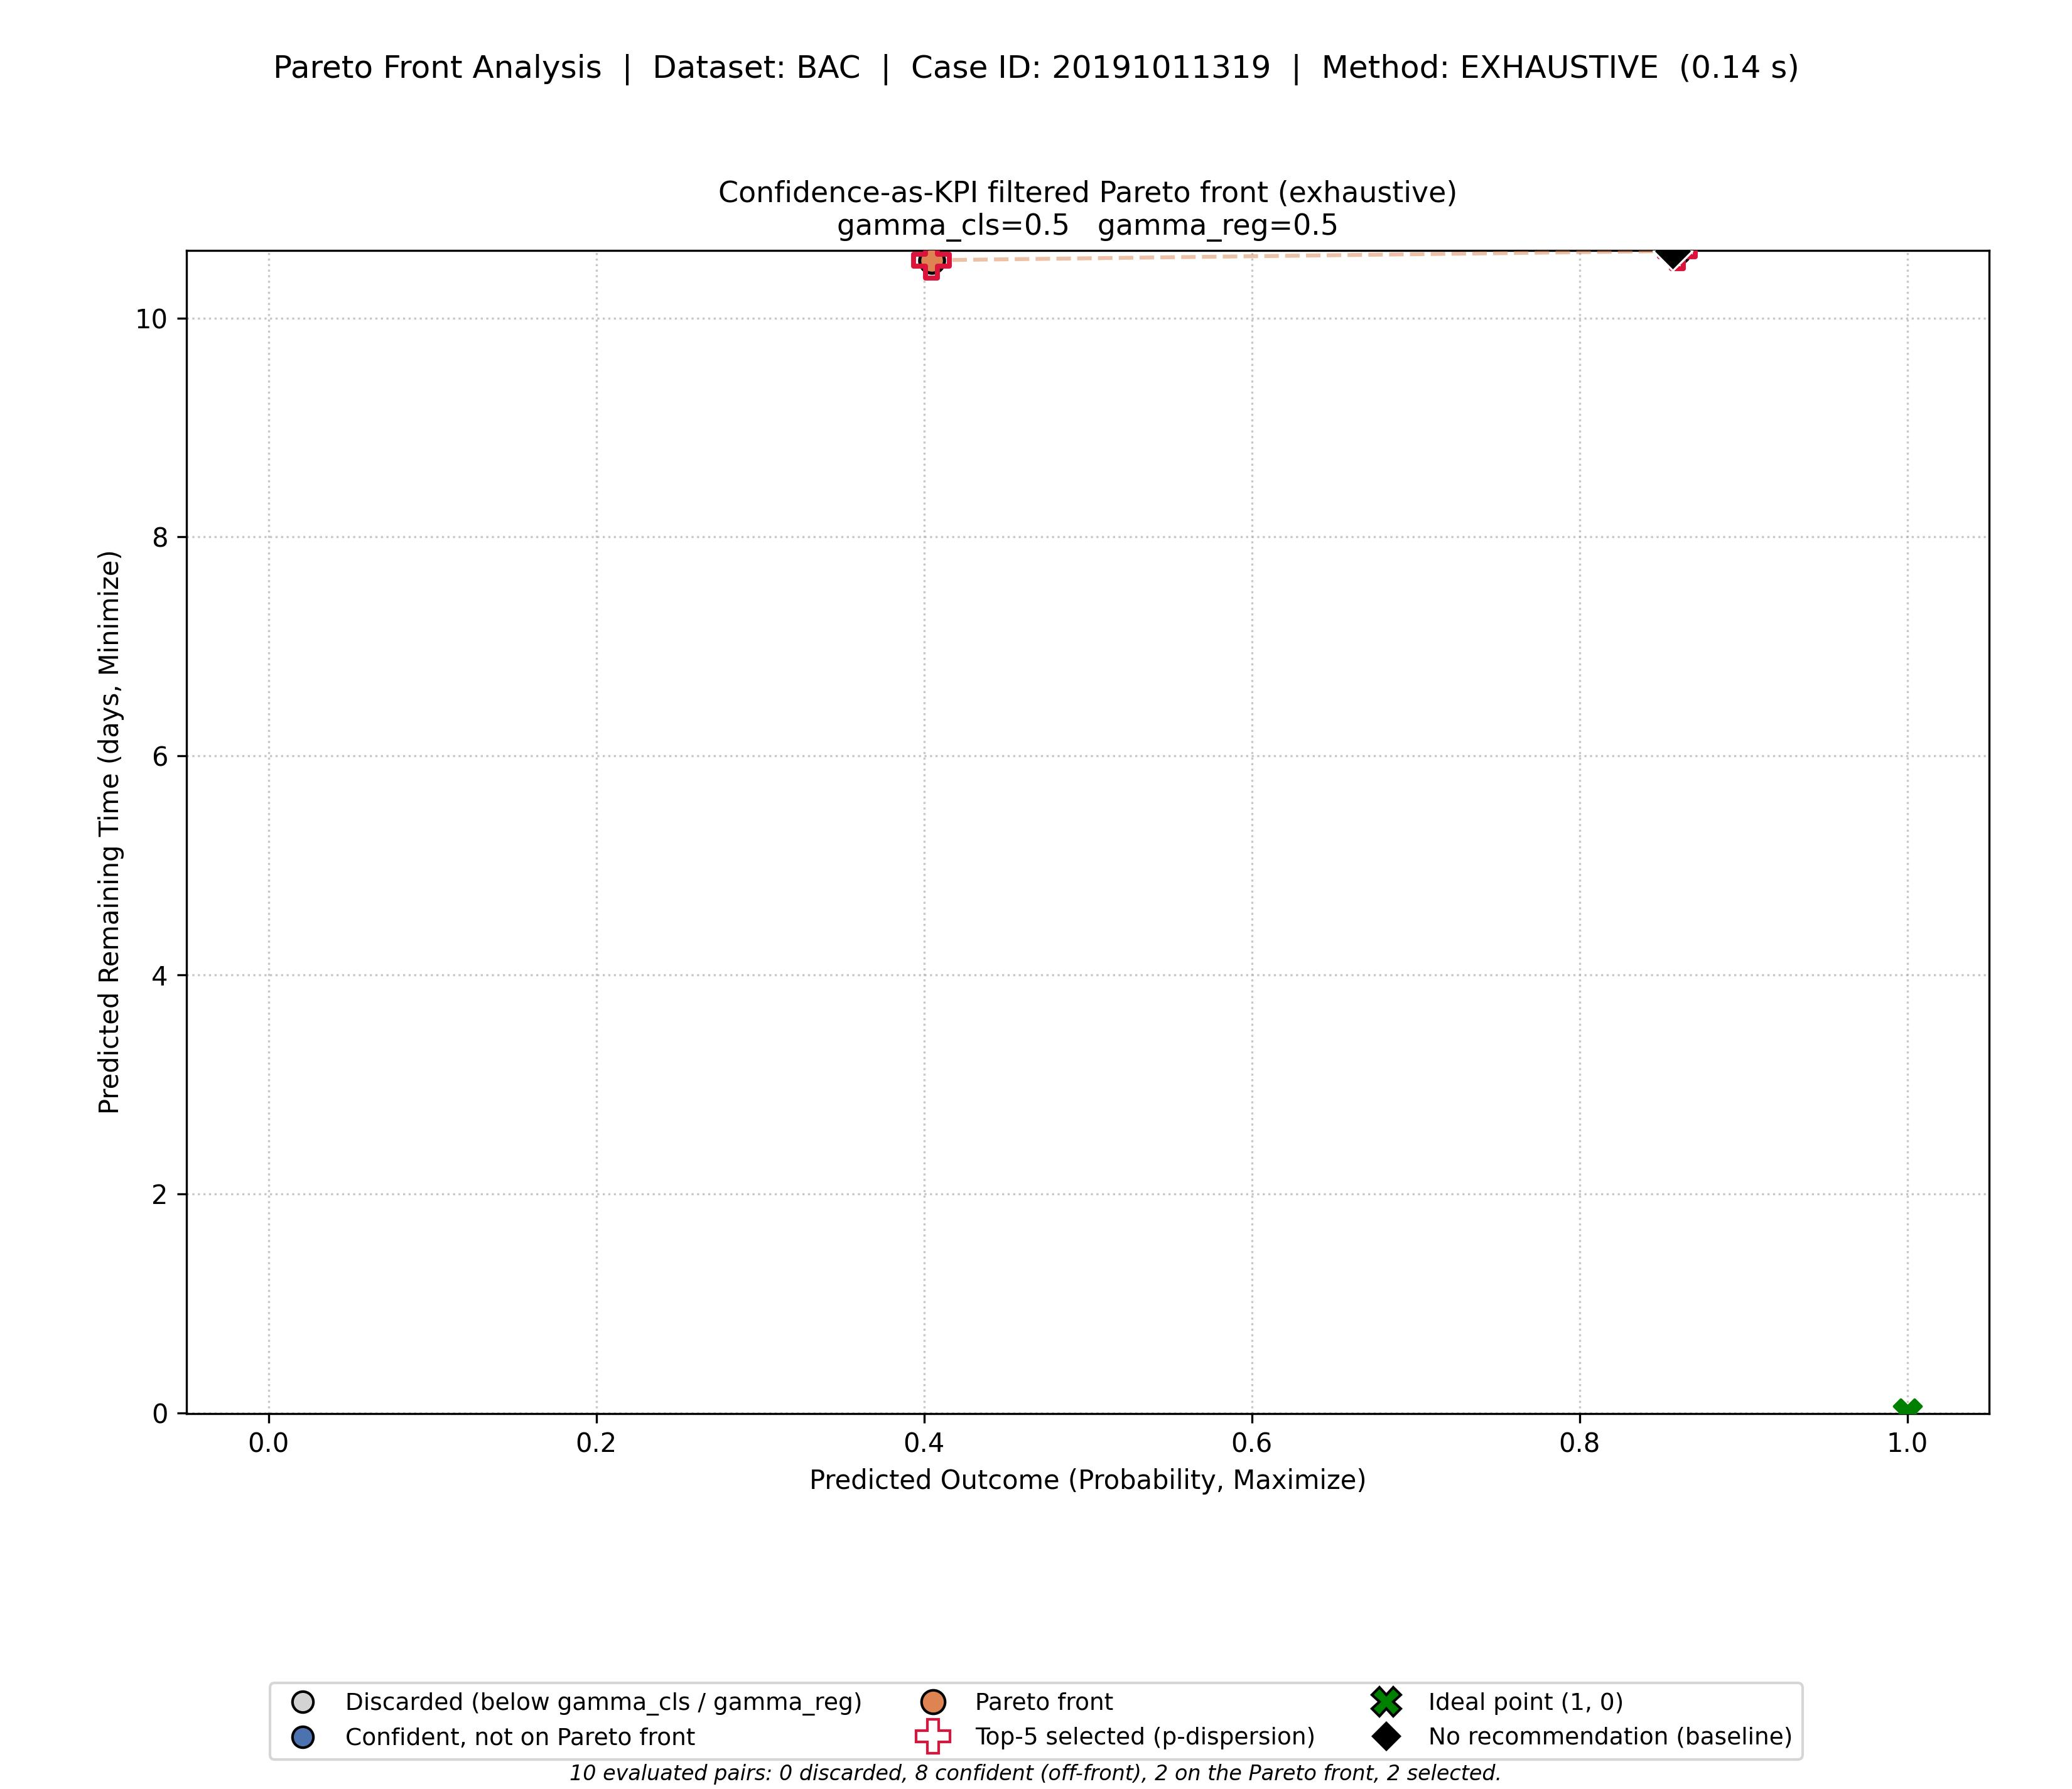
\includegraphics[width=0.5\linewidth]{multi_obj/pareto_fronts/pareto_fronts_dataset_predicted/BAC/pareto_BAC_20191011319_exhaustive.jpg}
    \end{figure}
\end{frame}

\begin{frame}{Experimental Results: Pareto Fronts (BPI12)}
    \begin{figure}
        \centering
        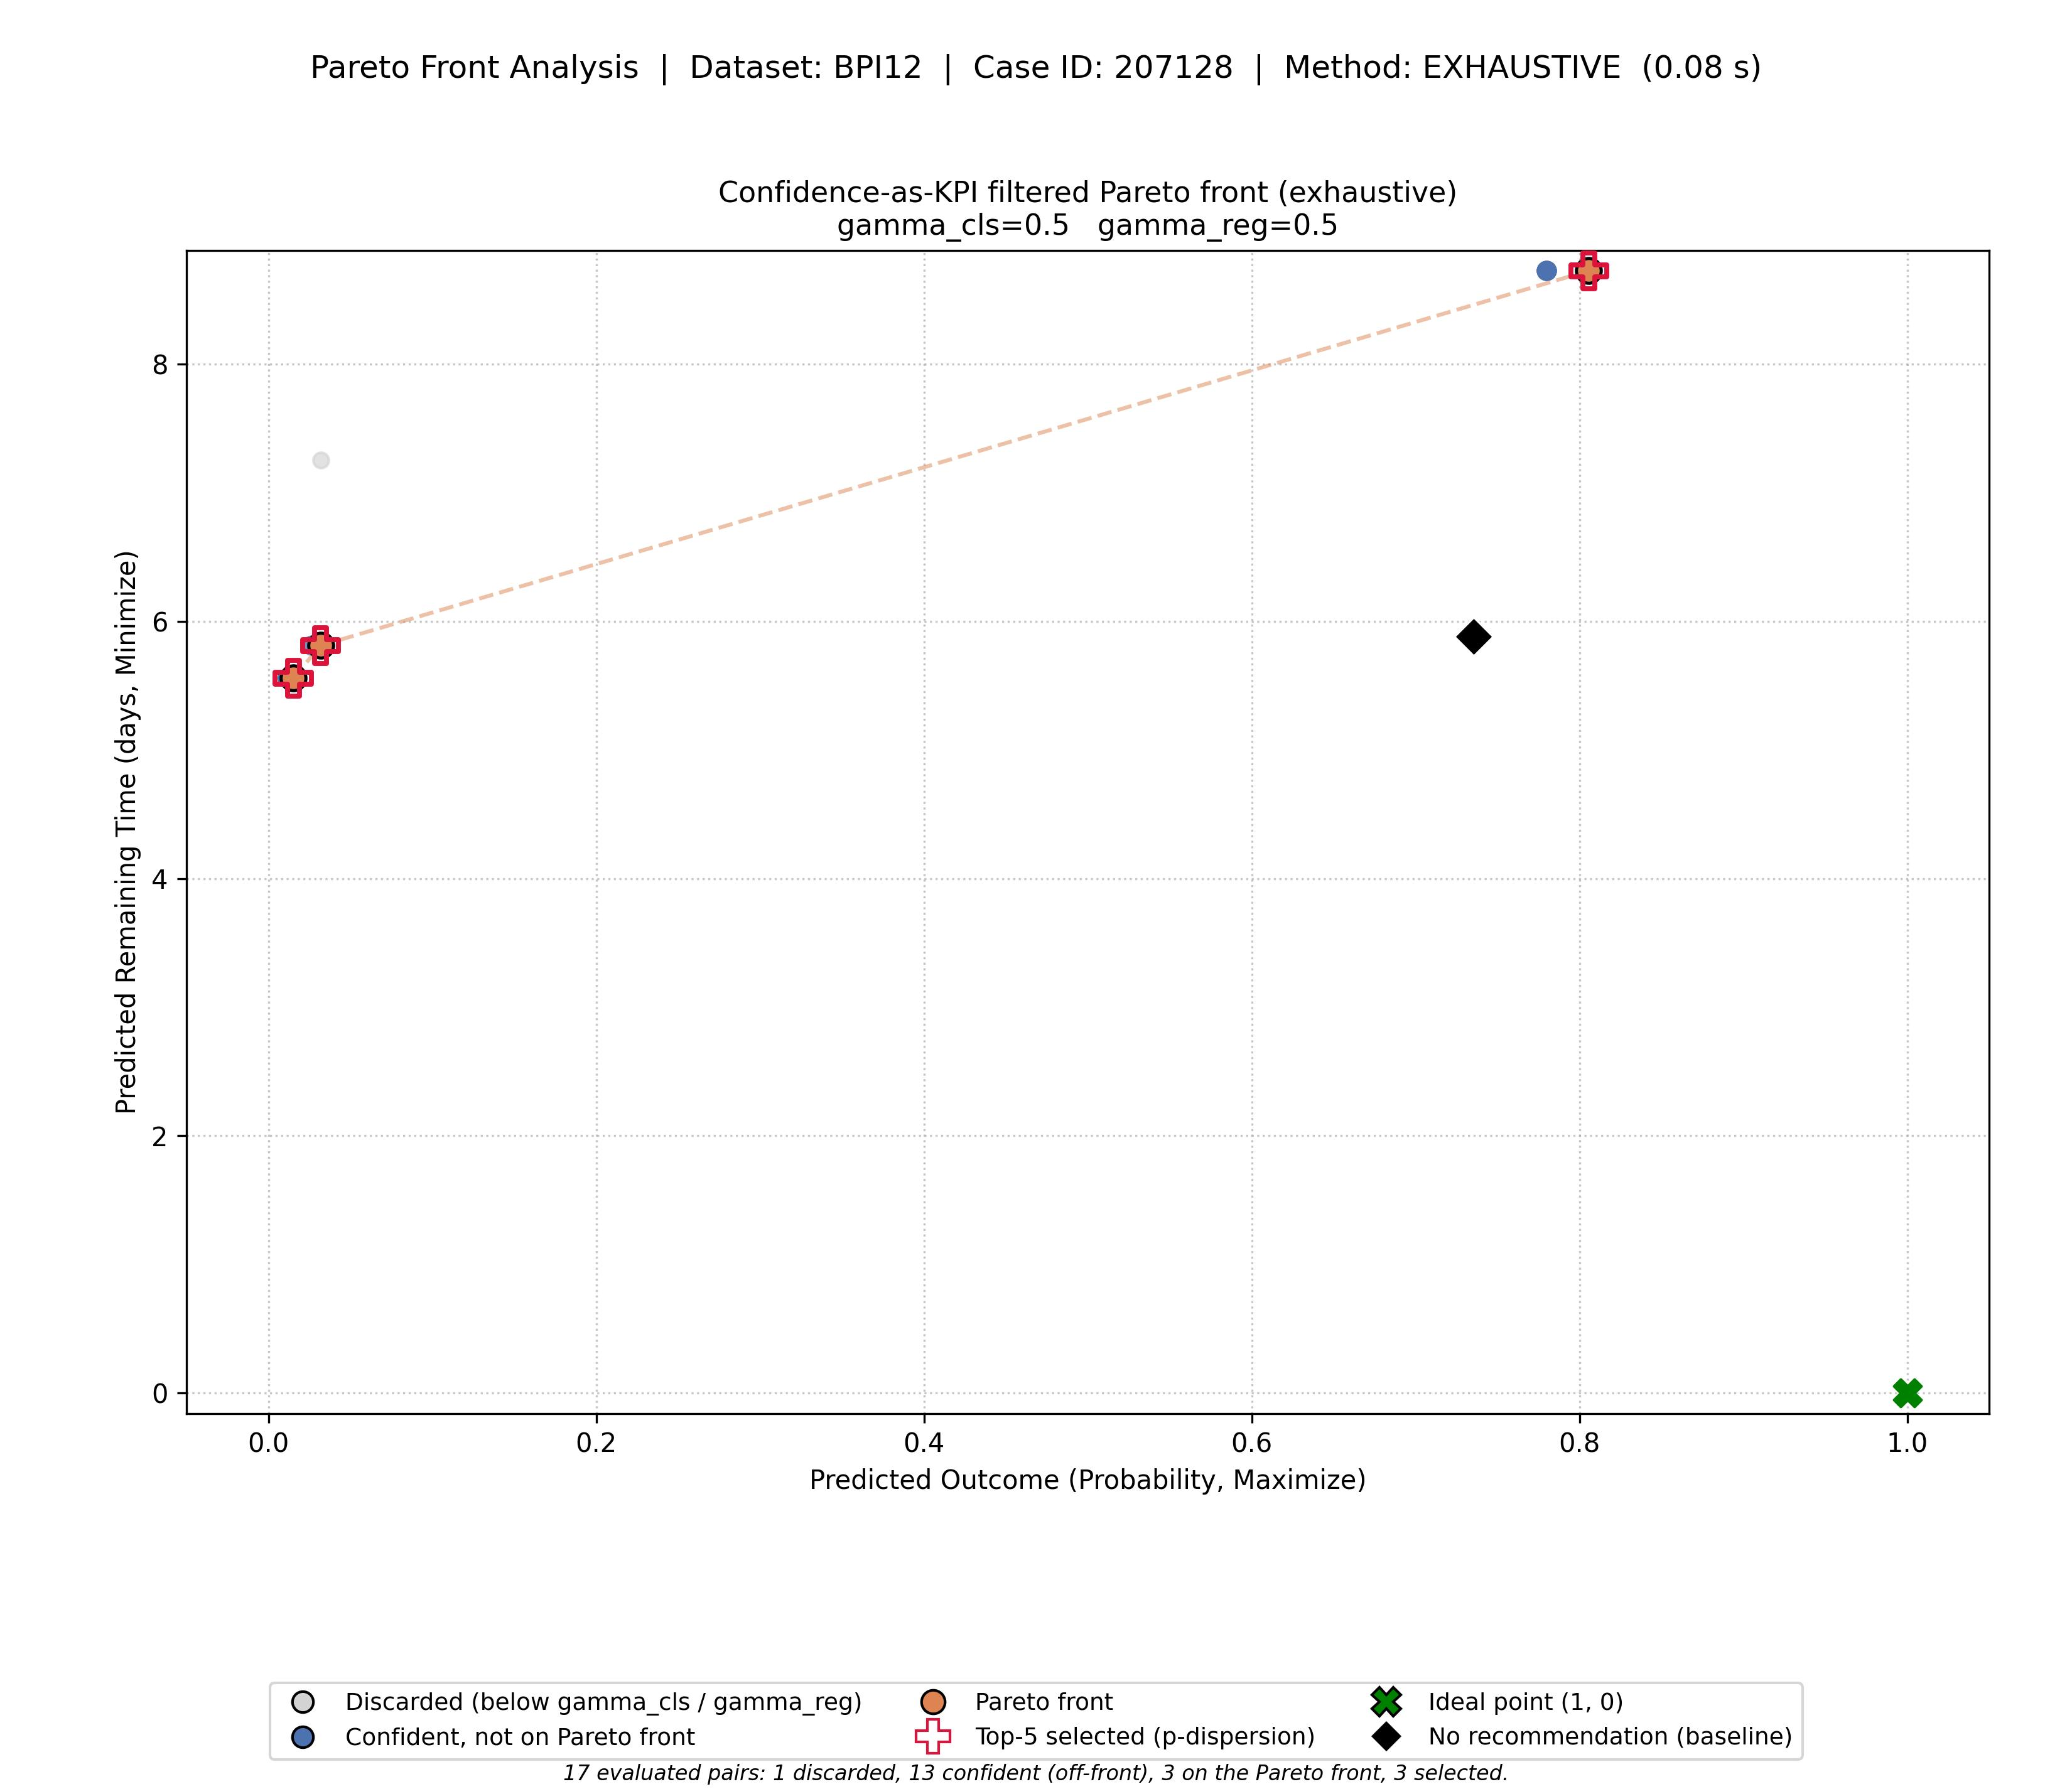
\includegraphics[width=0.5\linewidth]{multi_obj/pareto_fronts/pareto_fronts_dataset_predicted/BPI12/pareto_BPI12_207128_exhaustive.jpg}
    \end{figure}
\end{frame}

\begin{frame}{Experimental Results: Pareto Fronts (bpi17-before)}
    \begin{figure}
        \centering
        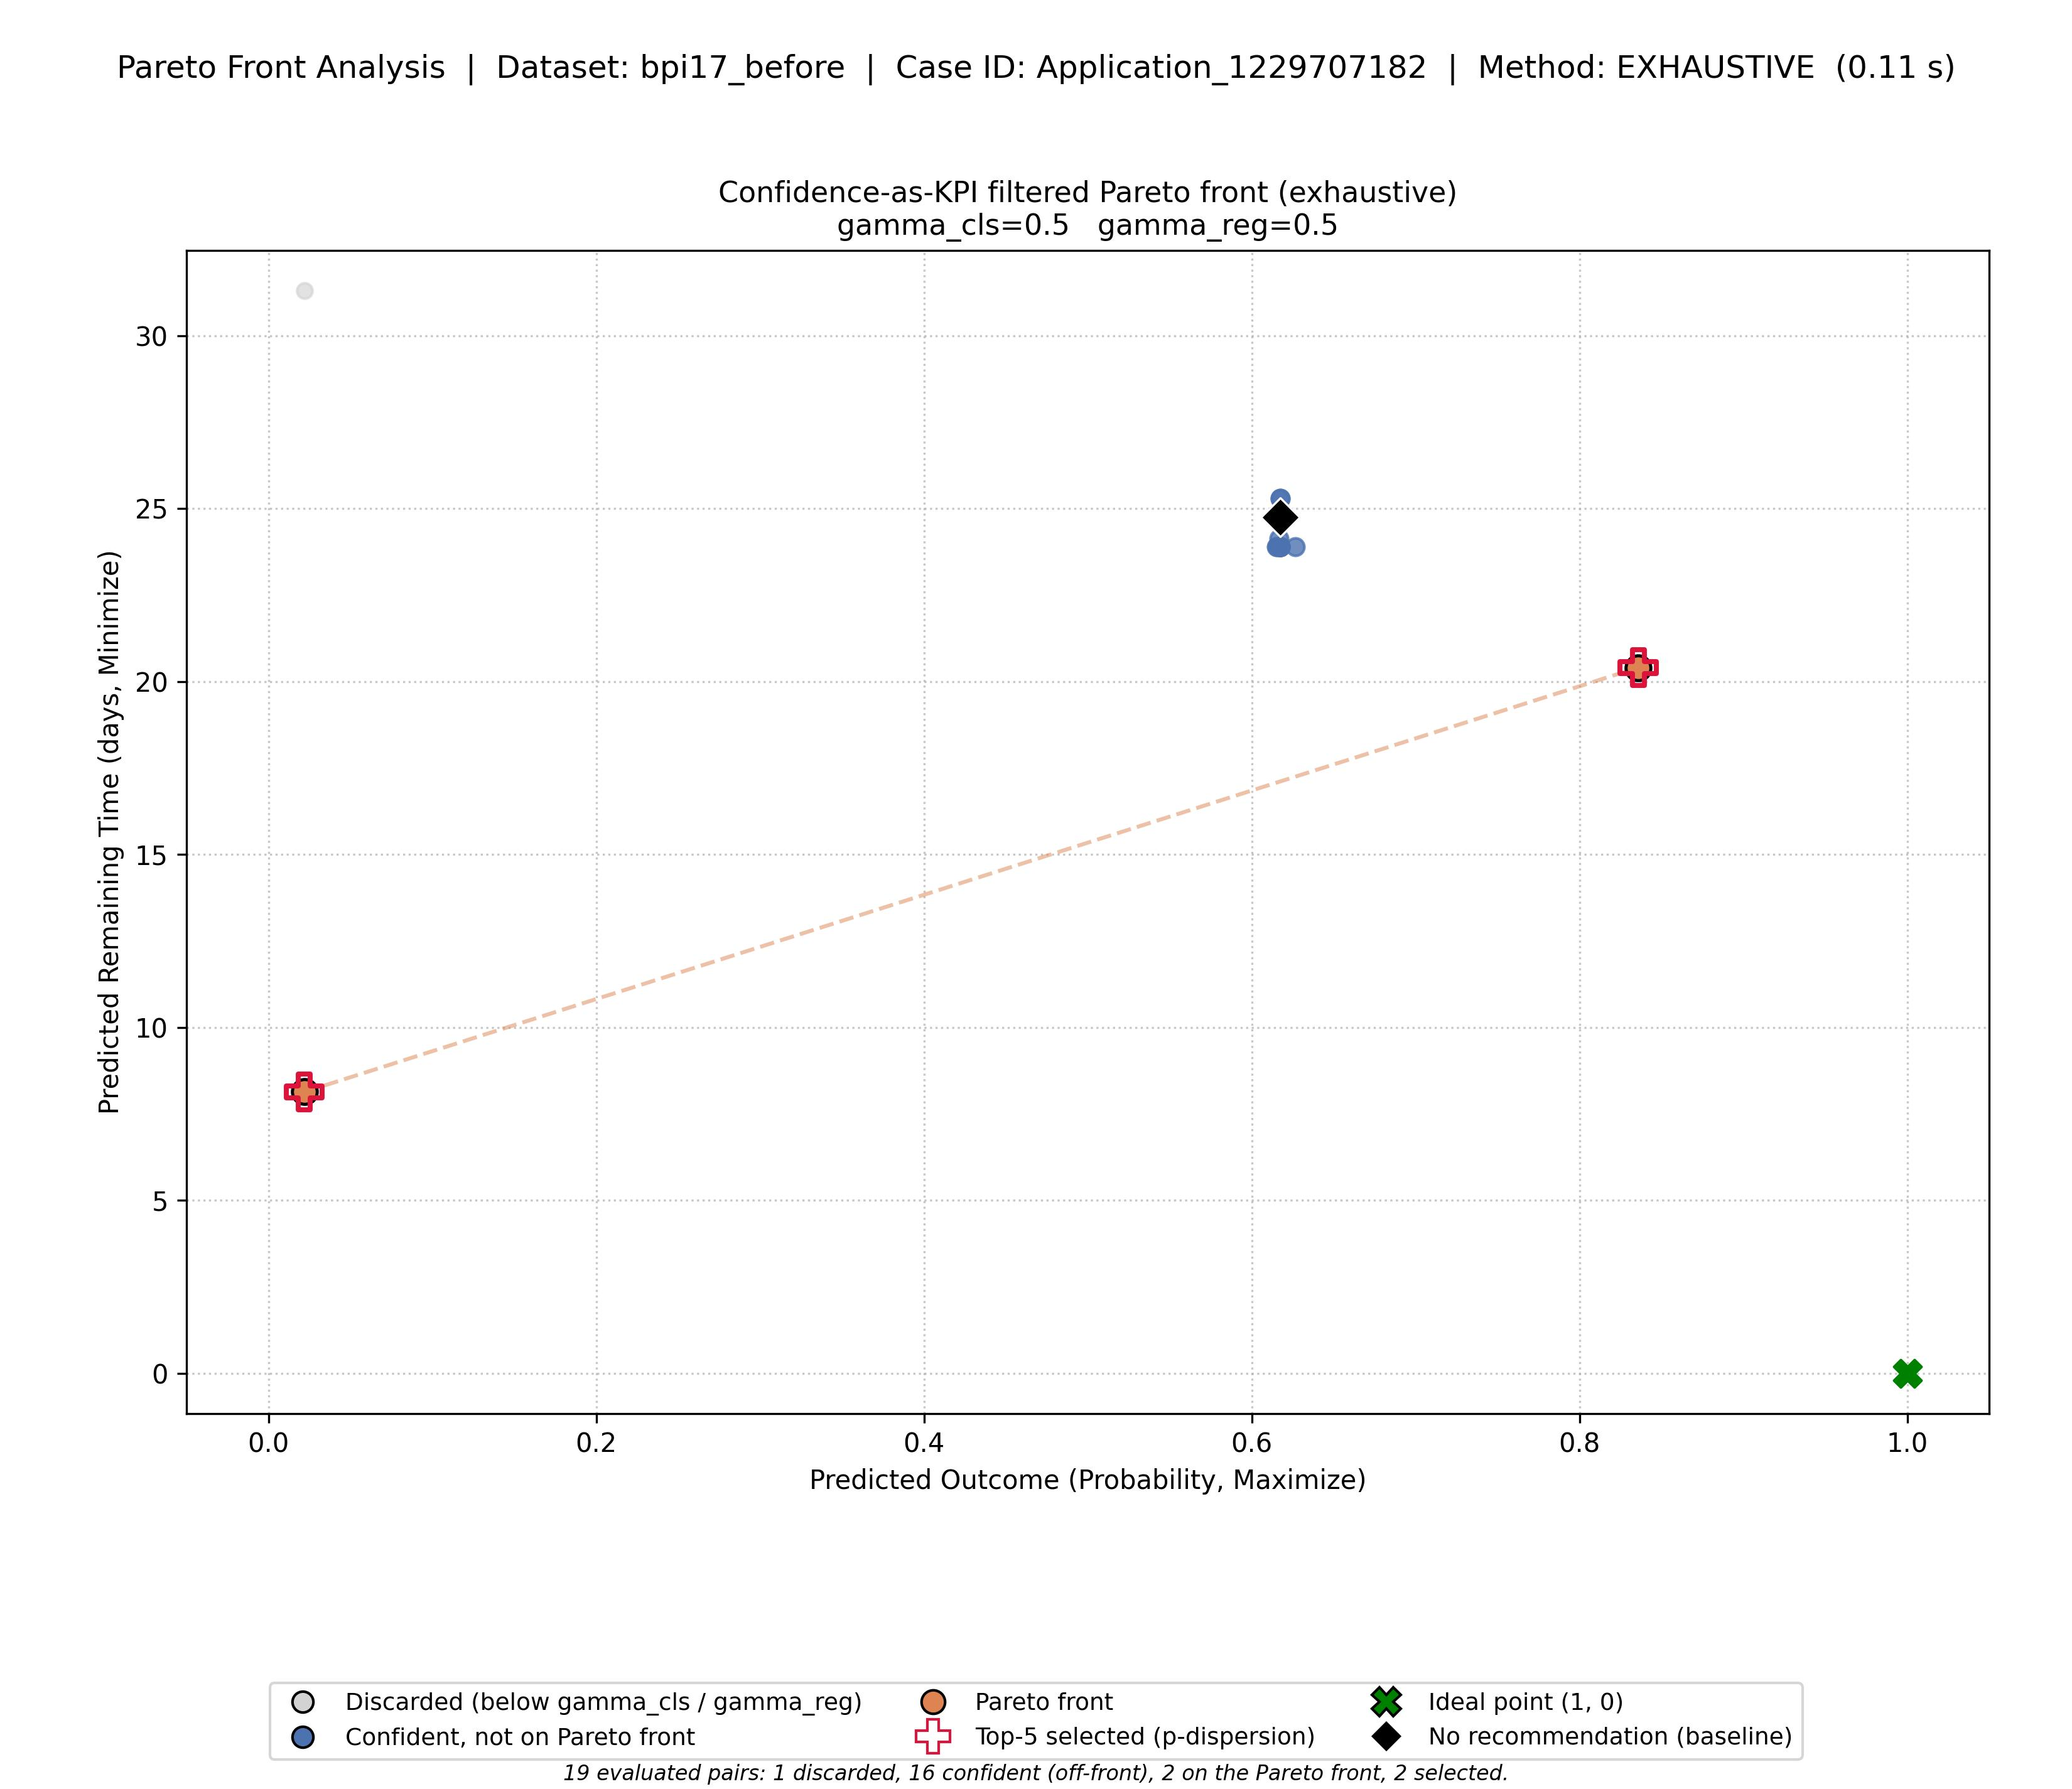
\includegraphics[width=0.5\linewidth]{multi_obj/pareto_fronts/pareto_fronts_dataset_predicted/bpi17_before/pareto_bpi17_before_Application_1229707182_exhaustive.jpg}
    \end{figure}
\end{frame}

\begin{frame}{Experimental Results: Pareto Fronts (bpi17-after)}
    \begin{figure}
        \centering
        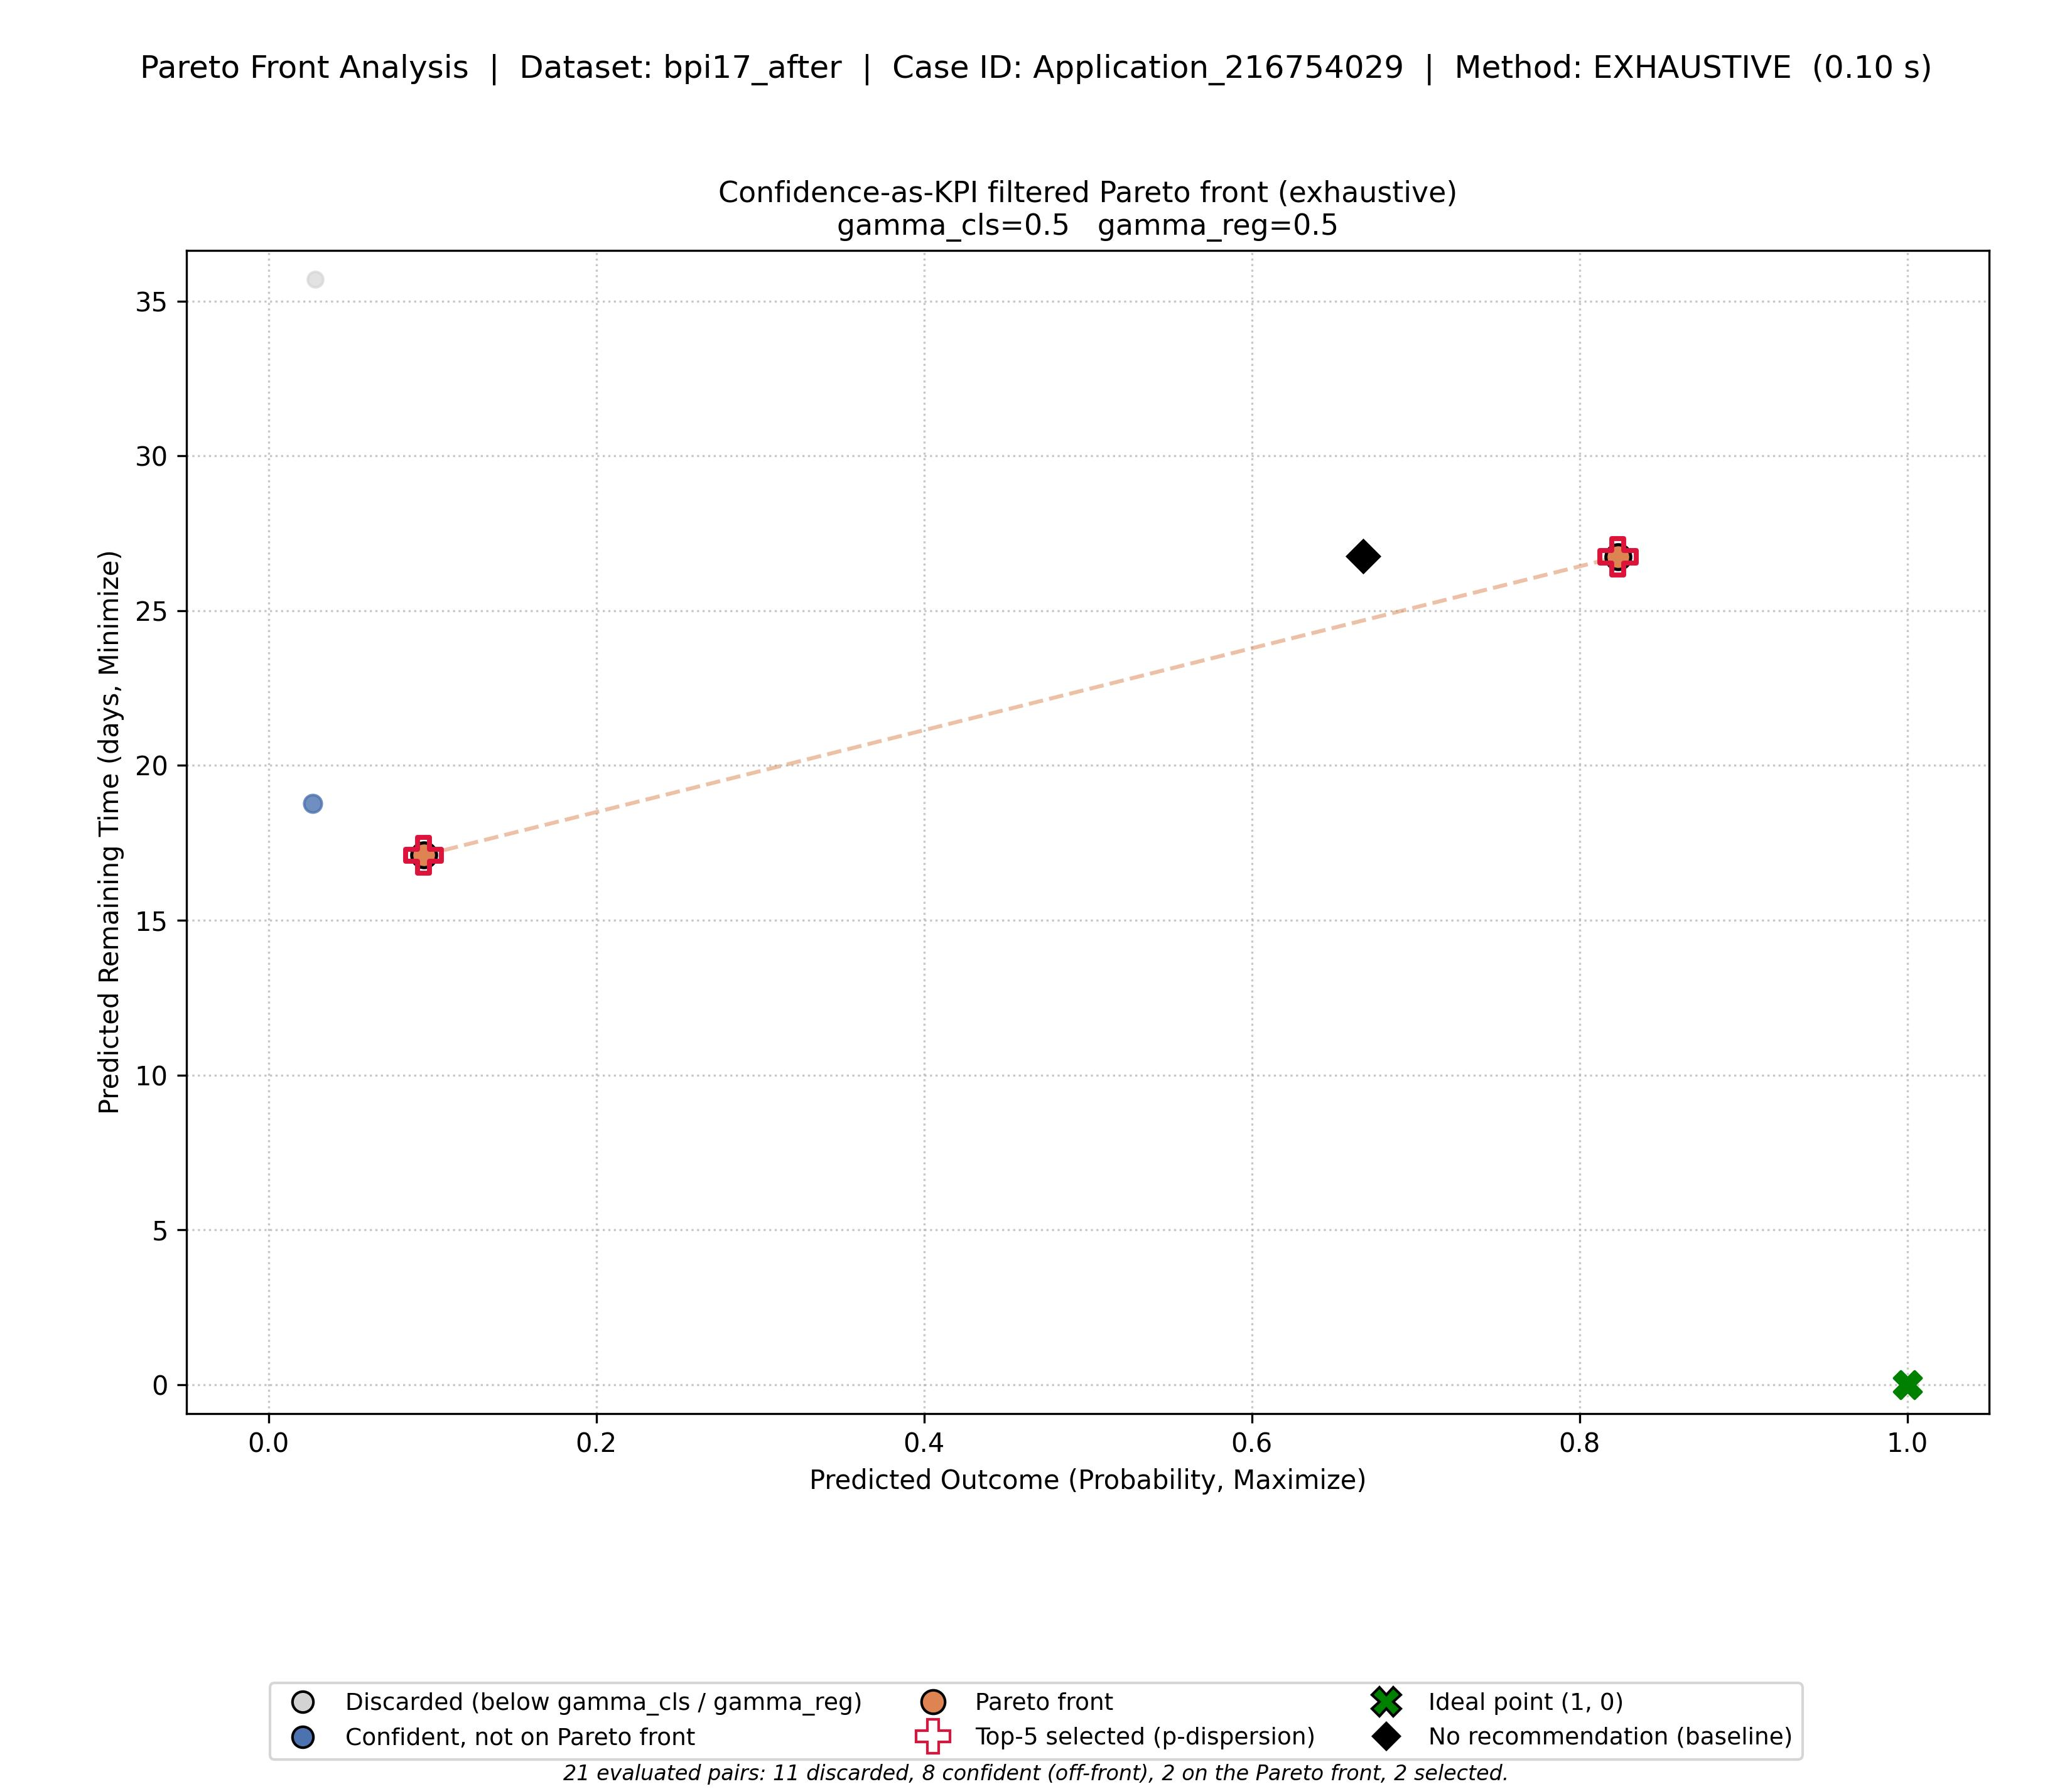
\includegraphics[width=0.5\linewidth]{multi_obj/pareto_fronts/pareto_fronts_dataset_predicted/bpi17_after/pareto_bpi17_after_Application_216754029_exhaustive.jpg}
    \end{figure}
\end{frame}

\begin{frame}{Pareto Front Cardinality}
    \begin{itemize}
        \item Not every case yields an equally rich Pareto front: the number of non-dominated (activity, resource) candidates strongly depends on how many feasible next steps exist at that point in the process.
        \item \textbf{Common pattern:} highly constrained states (few enabled transitions, few available resources) produce fronts with only a handful of points, sometimes even a single candidate.
        \item \textbf{Richer states:} early or highly flexible prefixes, with many enabled activity/resource combinations, tend to produce larger and more diverse fronts.
        \item This variability is handled directly by the selection rule described next, which naturally adapts to fronts of any size.
    \end{itemize}
    % TODO: add follow-up slides here with example Pareto fronts of small cardinality
\end{frame}

\begin{frame}{Experimental Results: Pareto Fronts Cardinality examples (BAC)}
    \centering

    \begin{minipage}{0.48\textwidth}
        \centering
        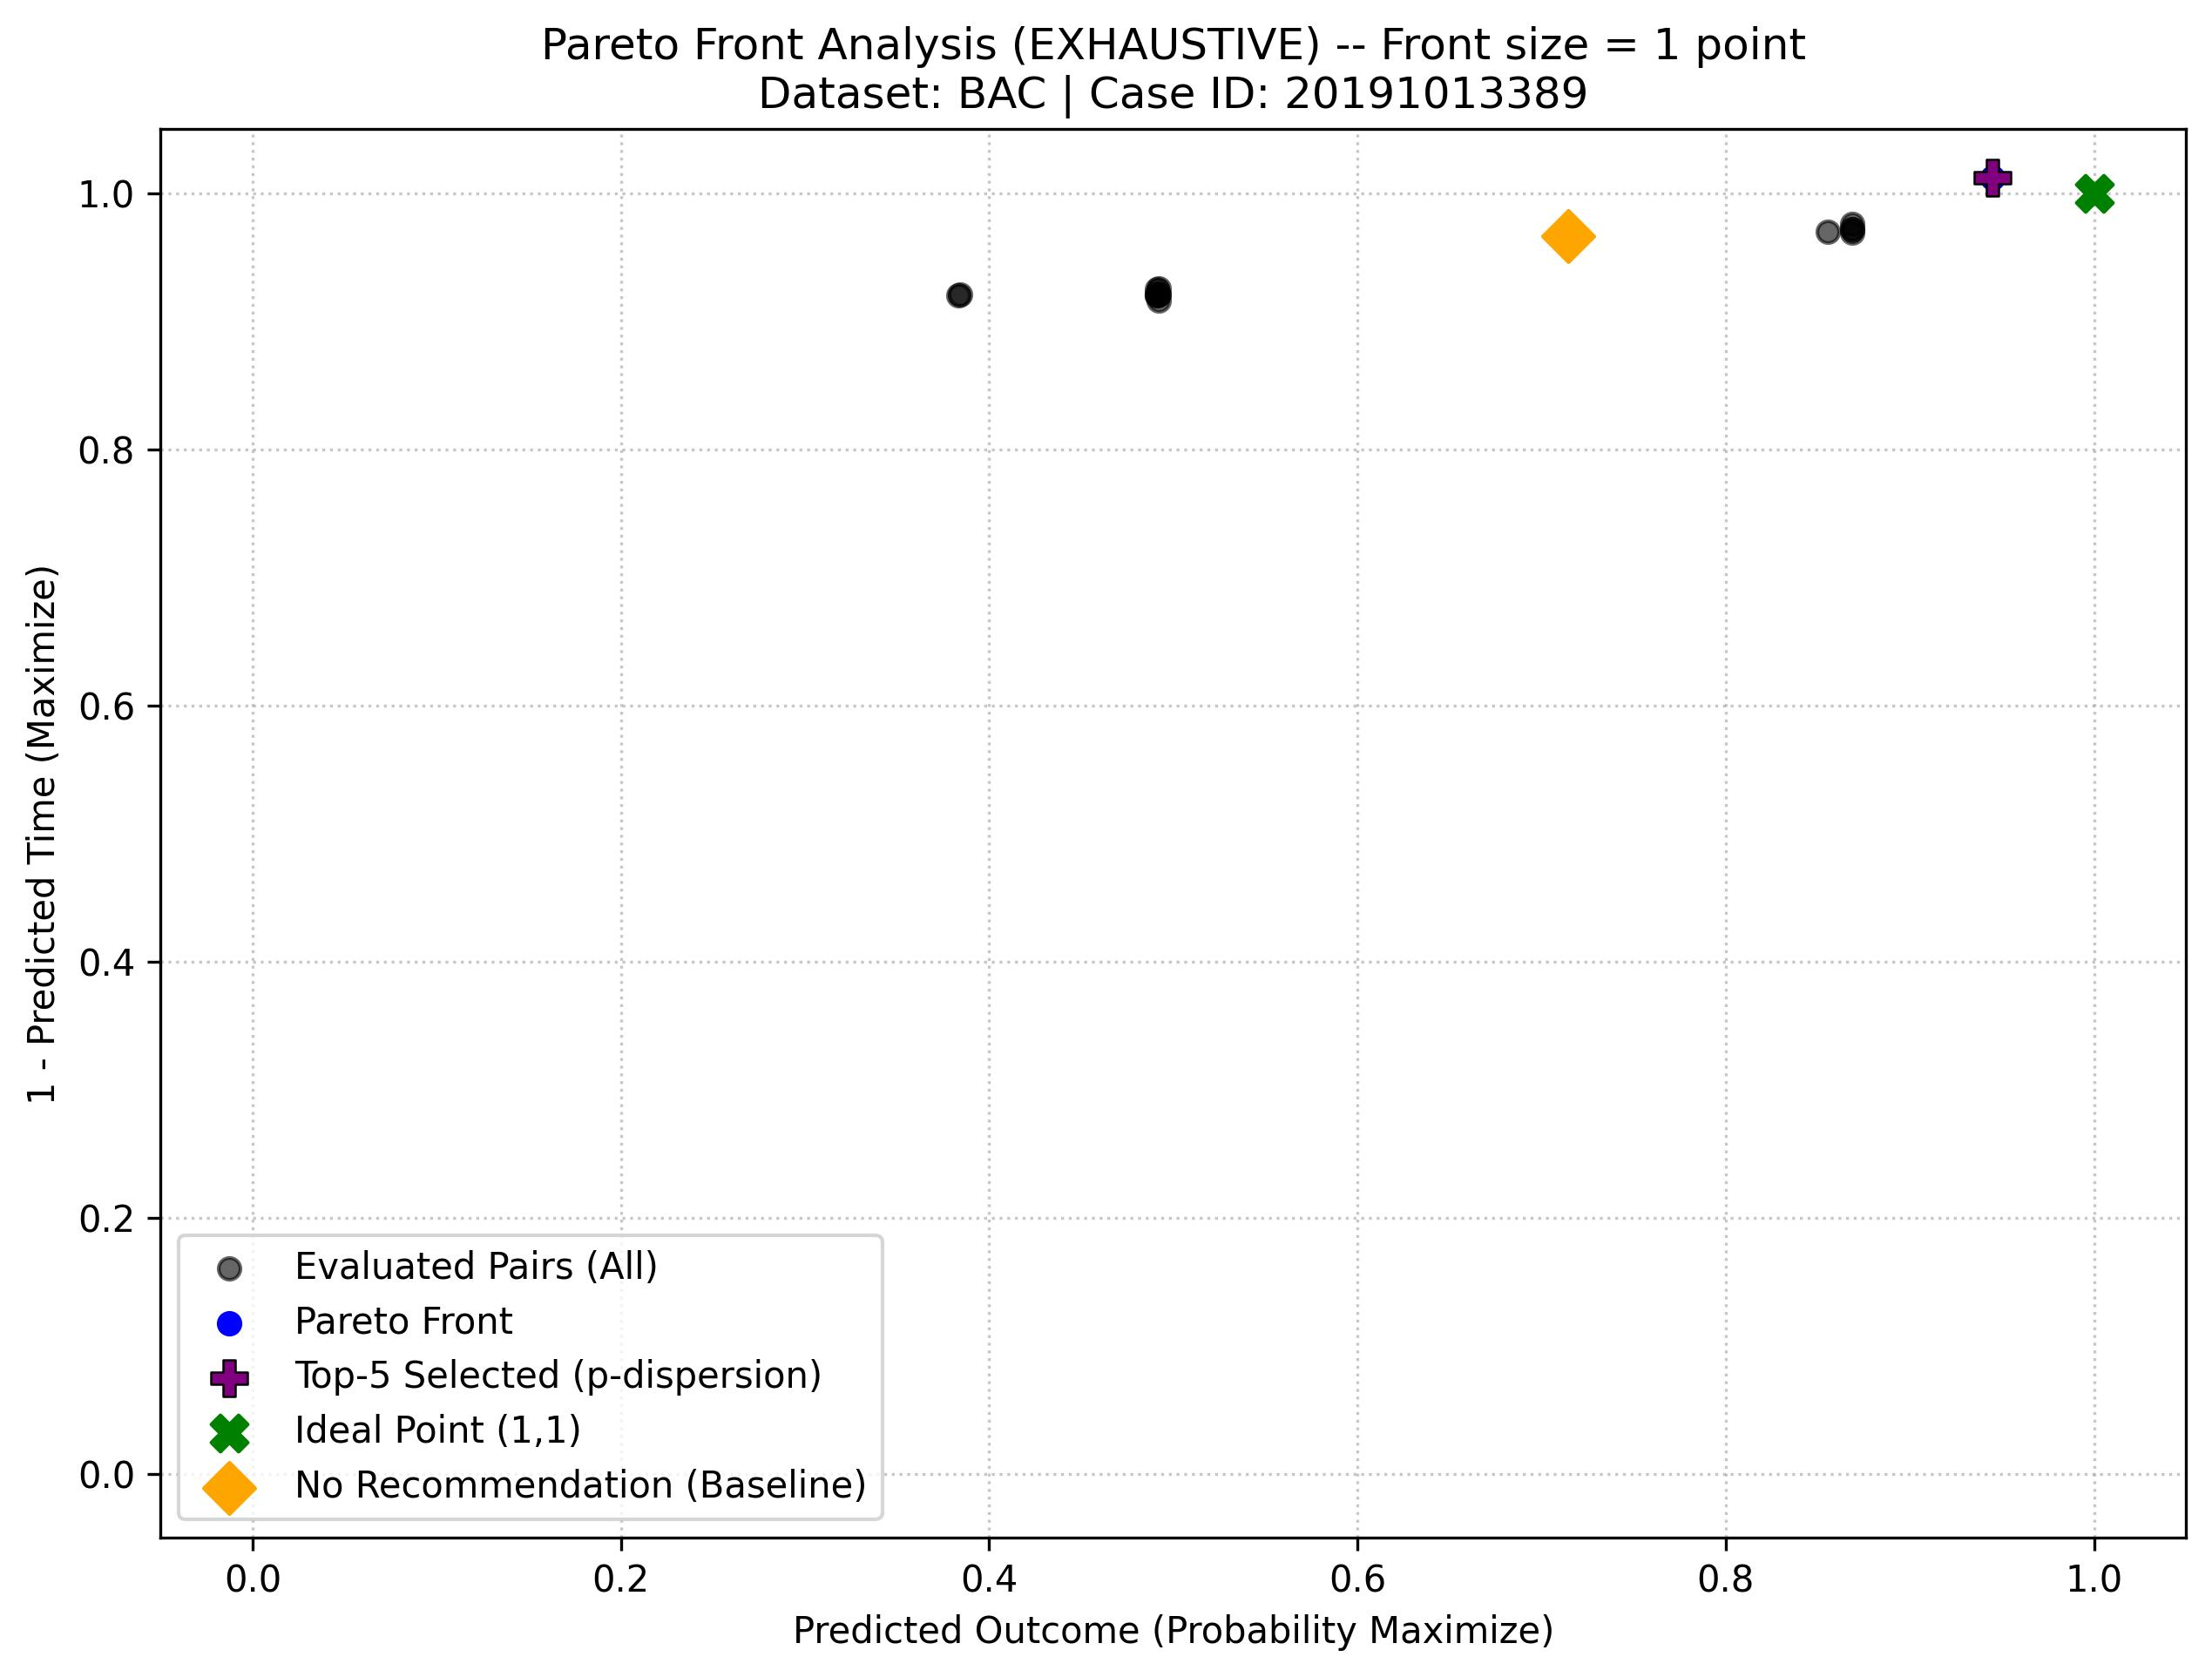
\includegraphics[width=1.03\linewidth]{multi_obj/pareto_fronts/pareto_front_size_examples/pareto_BAC_frontsize_1_20191013389.jpg}
    \end{minipage}
    \begin{minipage}{0.48\textwidth}
        \centering
        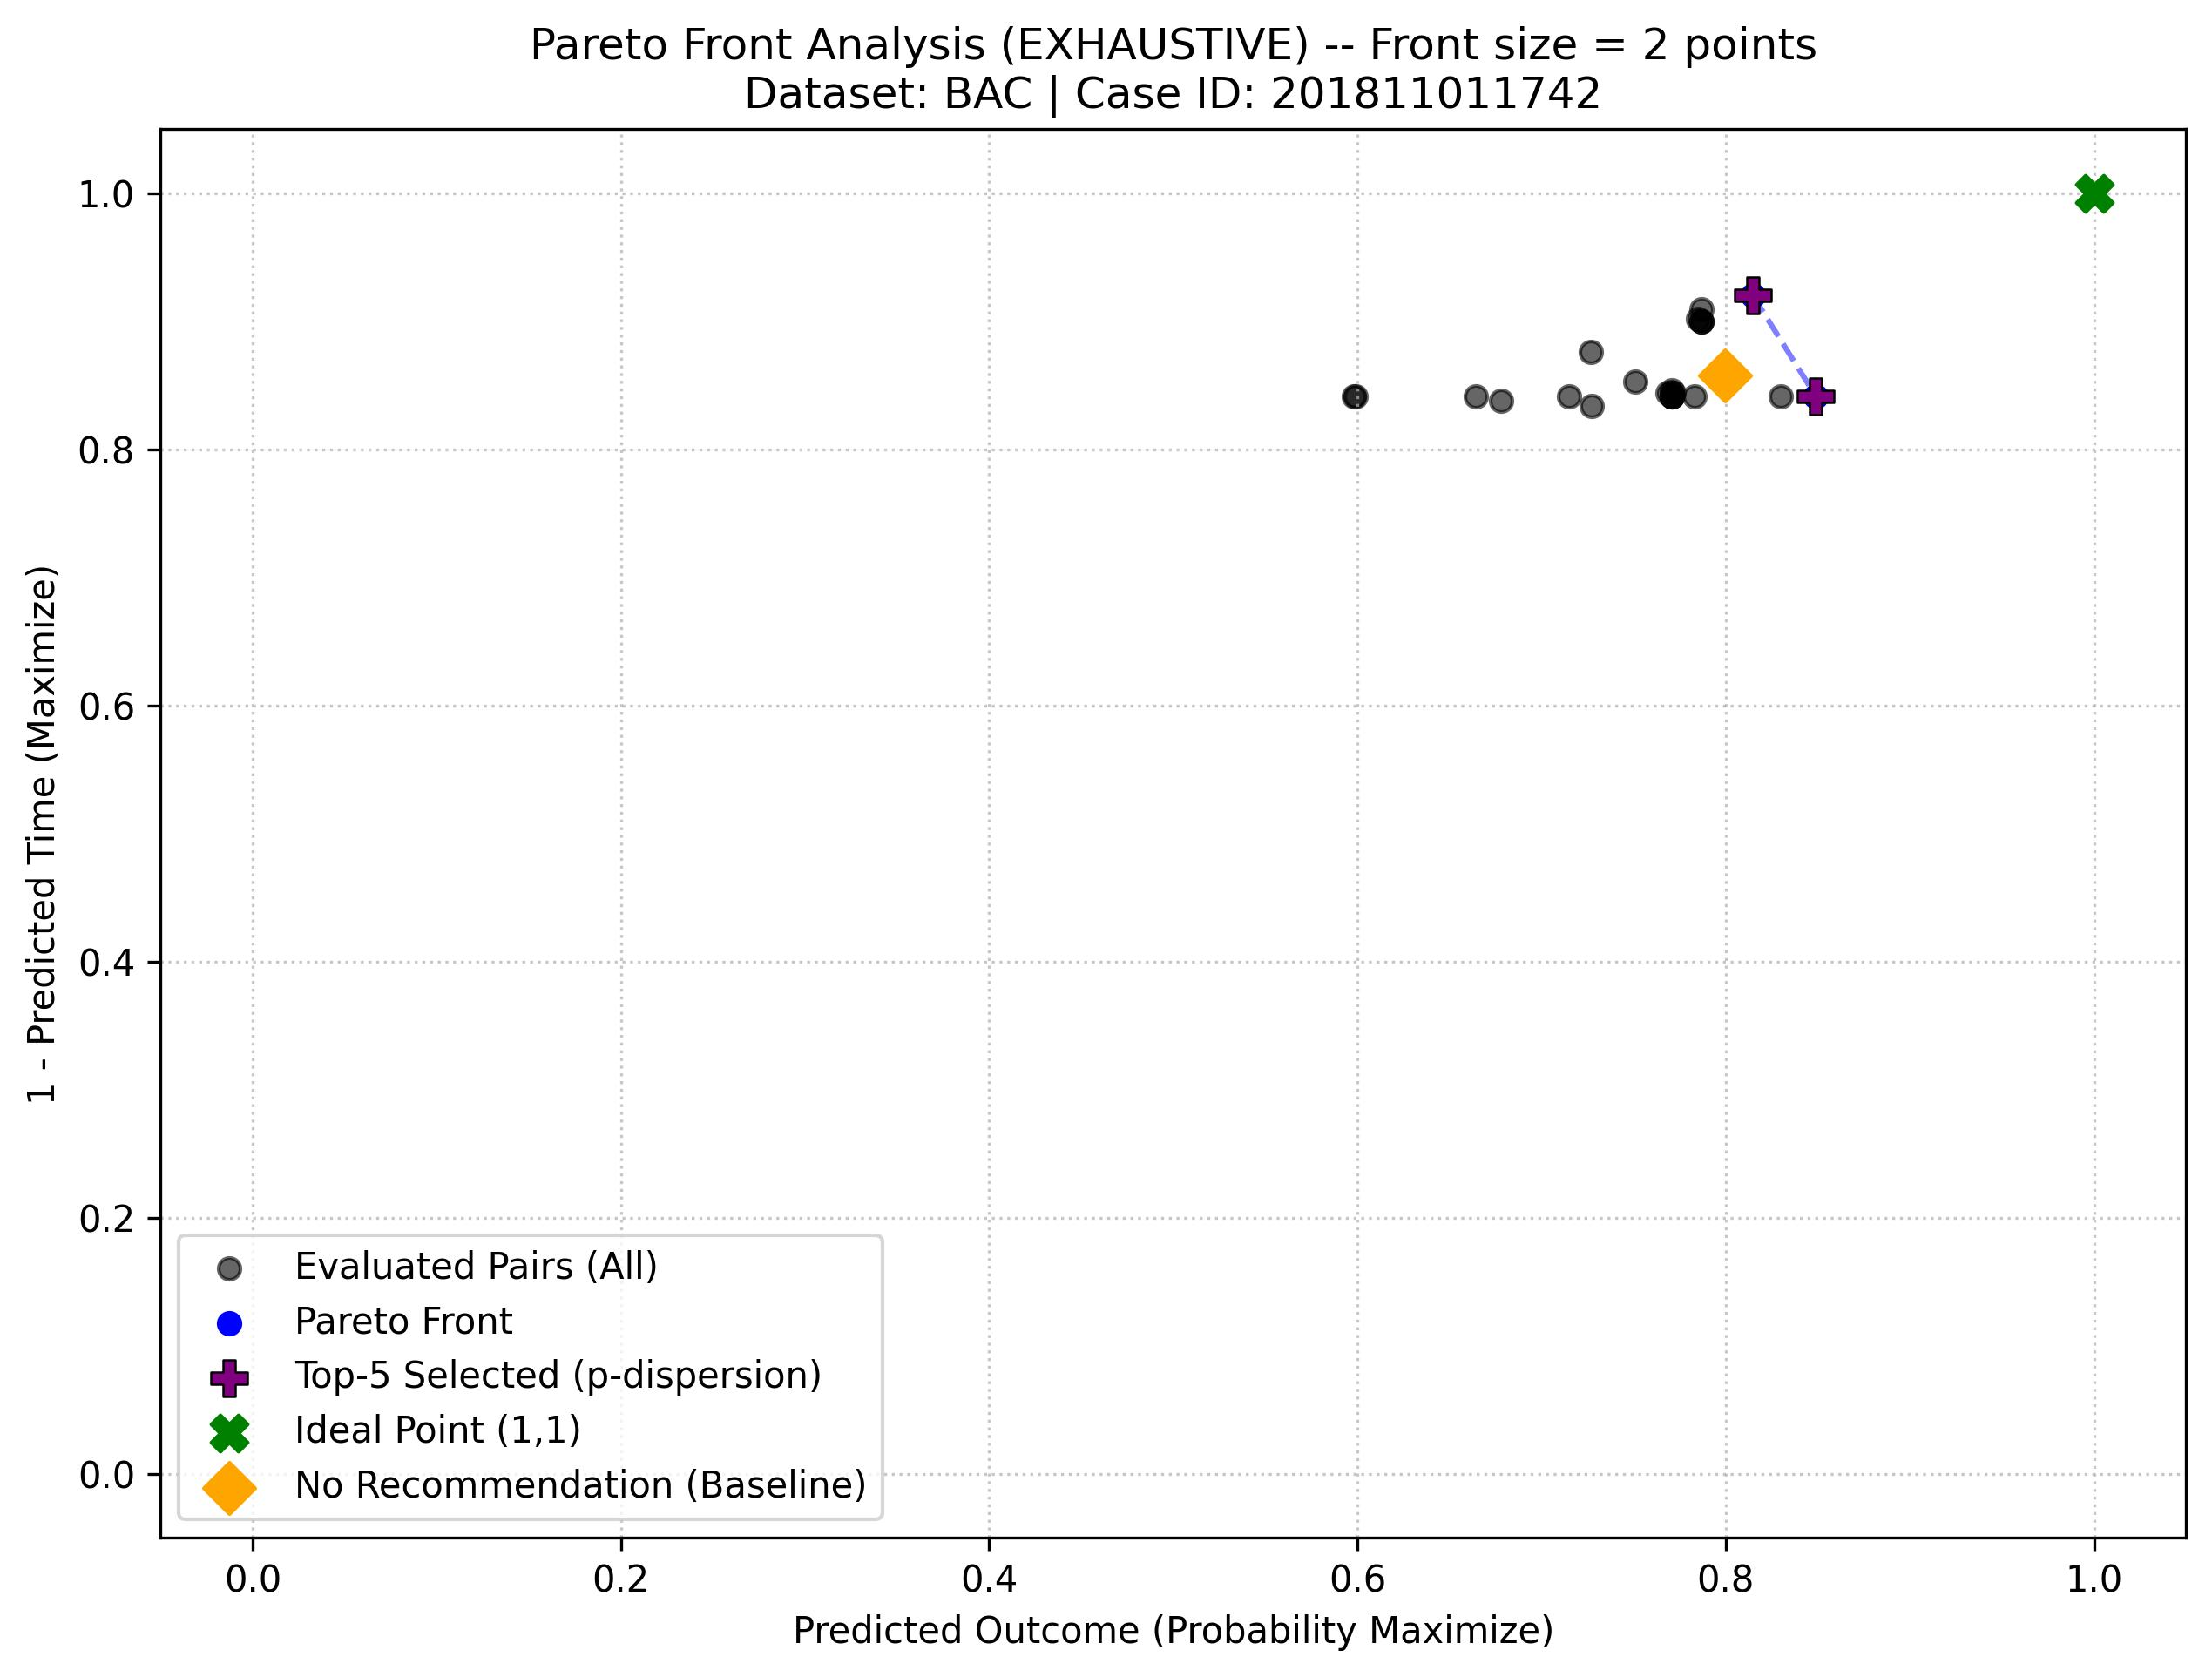
\includegraphics[width=1.03\linewidth]{multi_obj/pareto_fronts/pareto_front_size_examples/pareto_BAC_frontsize_2_201811011742.jpg}
    \end{minipage}

\end{frame}

\begin{frame}{Experimental Results: Pareto Fronts Cardinality examples (BAC)}
    \centering

    \begin{minipage}{0.48\textwidth}
        \centering
        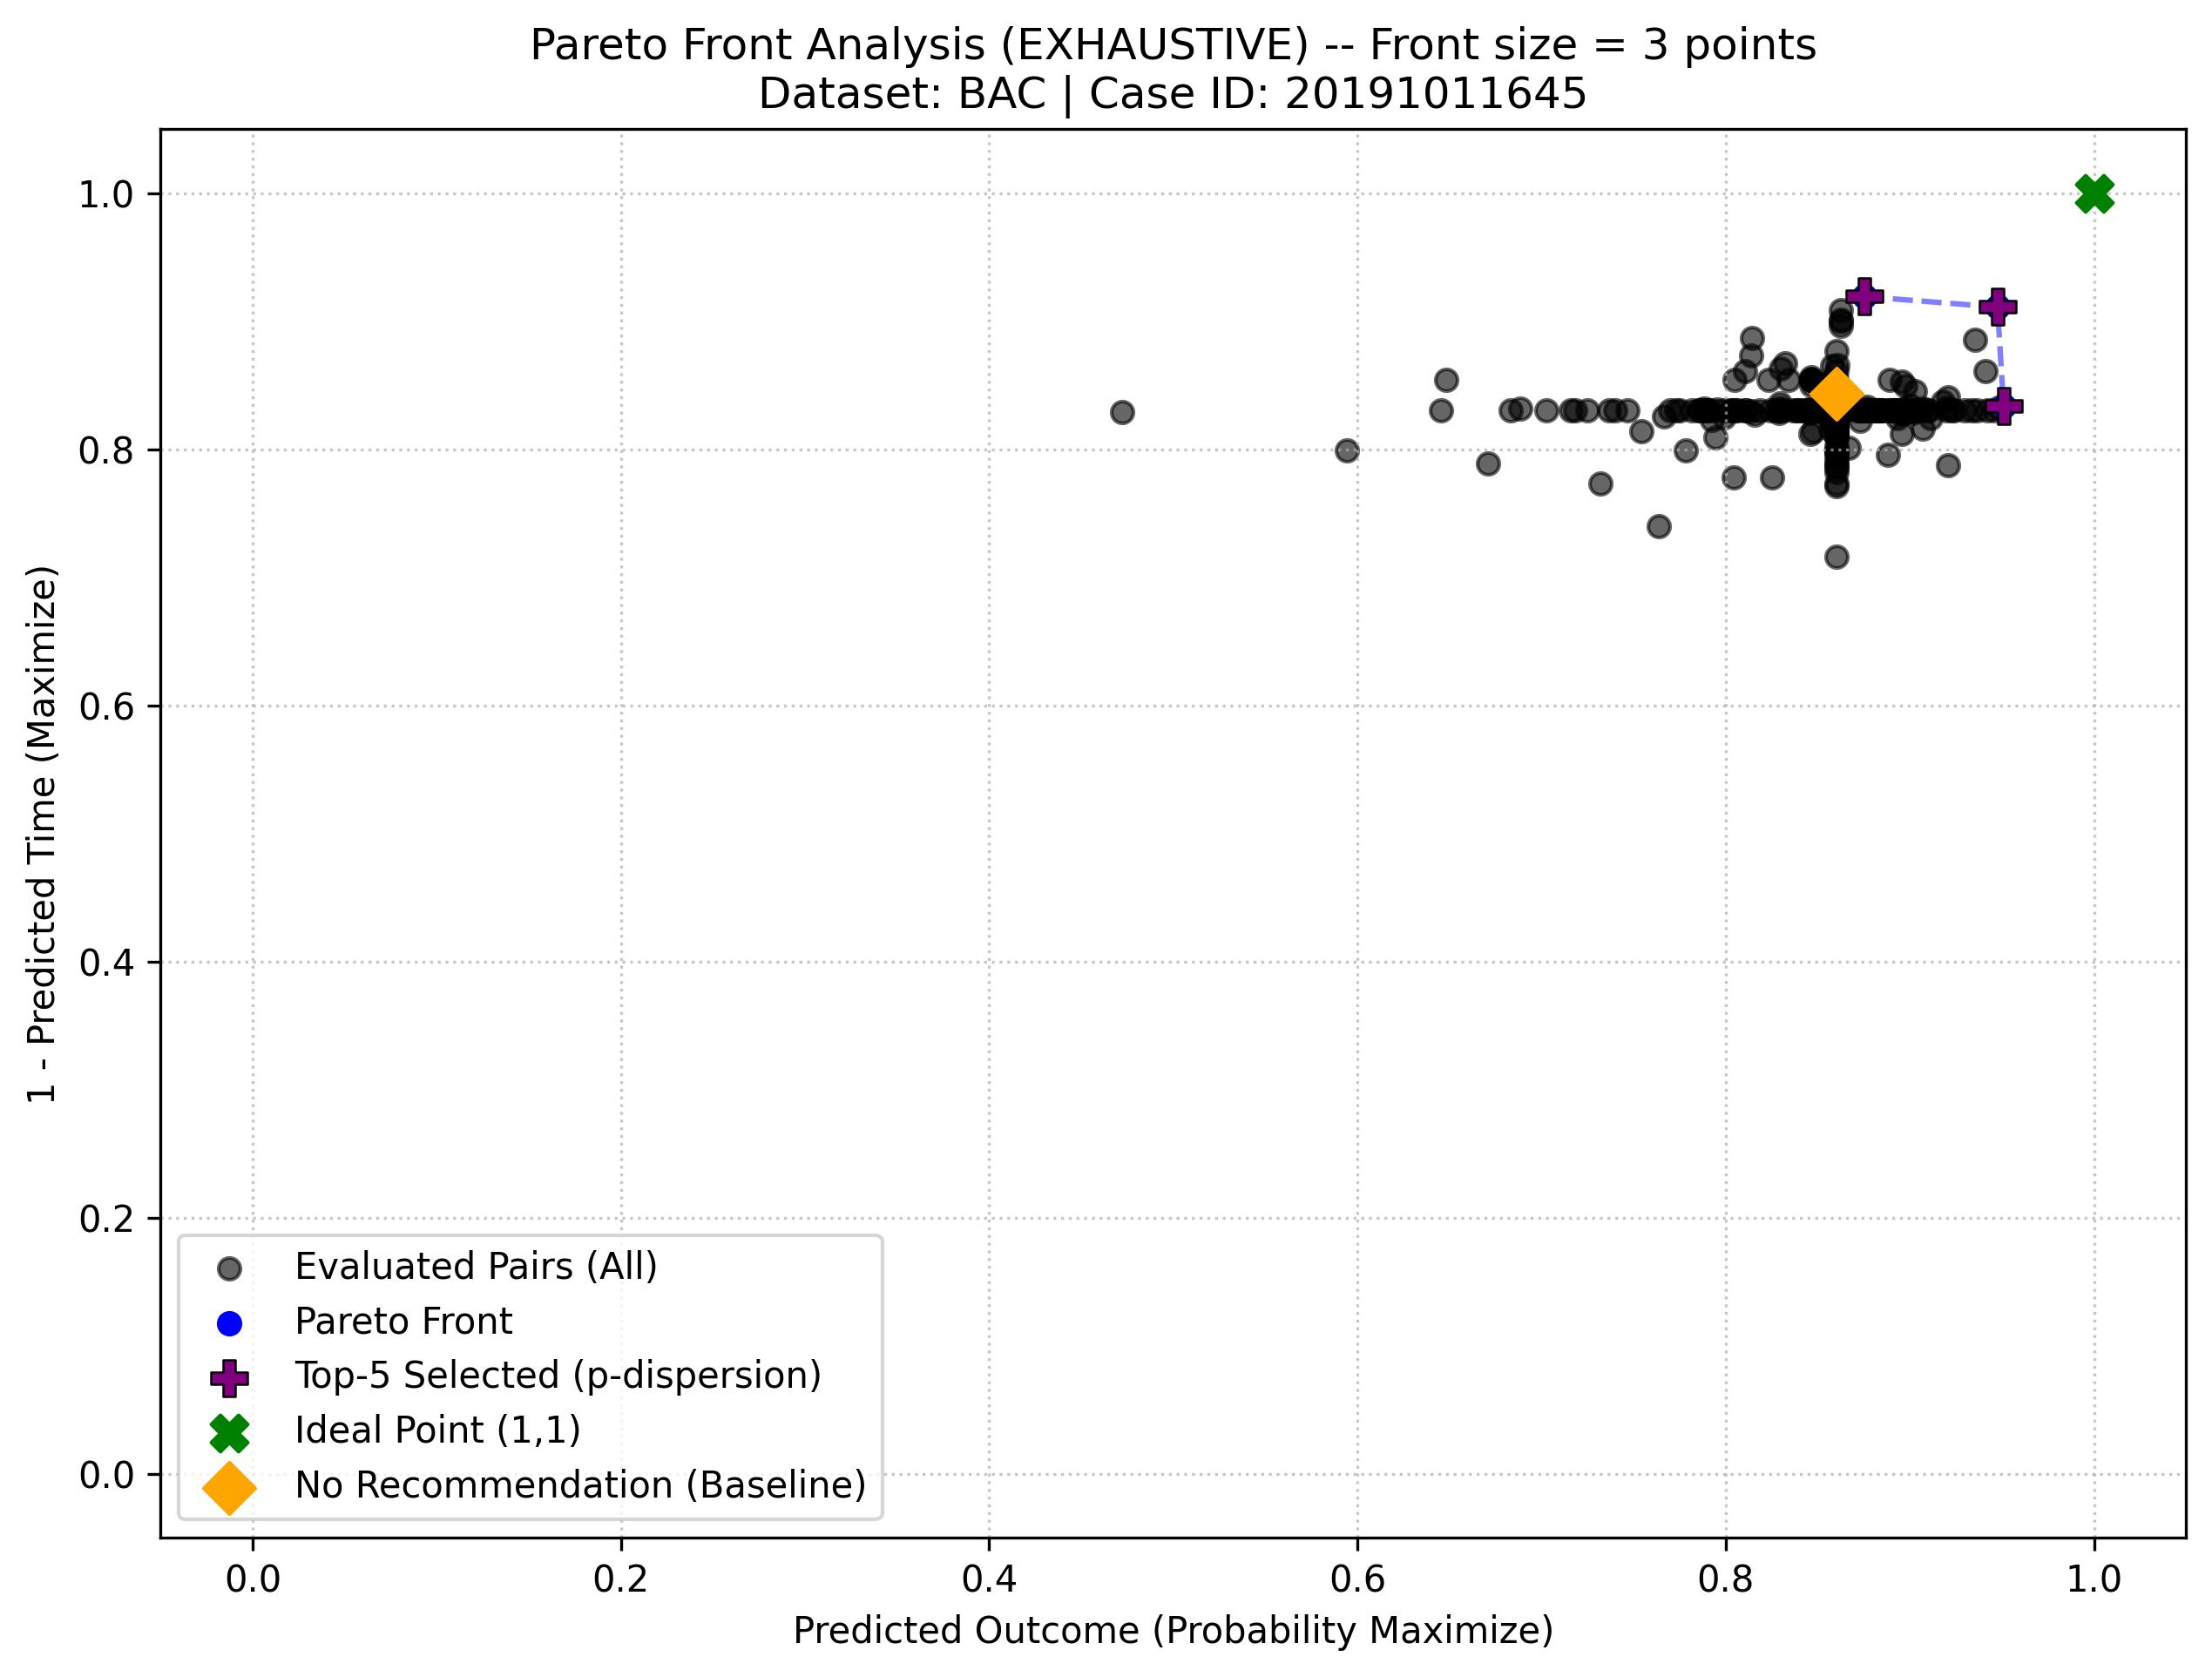
\includegraphics[width=1.03\linewidth]{multi_obj/pareto_fronts/pareto_front_size_examples/pareto_BAC_frontsize_3_20191011645.jpg}
    \end{minipage}
    \begin{minipage}{0.48\textwidth}
        \centering
        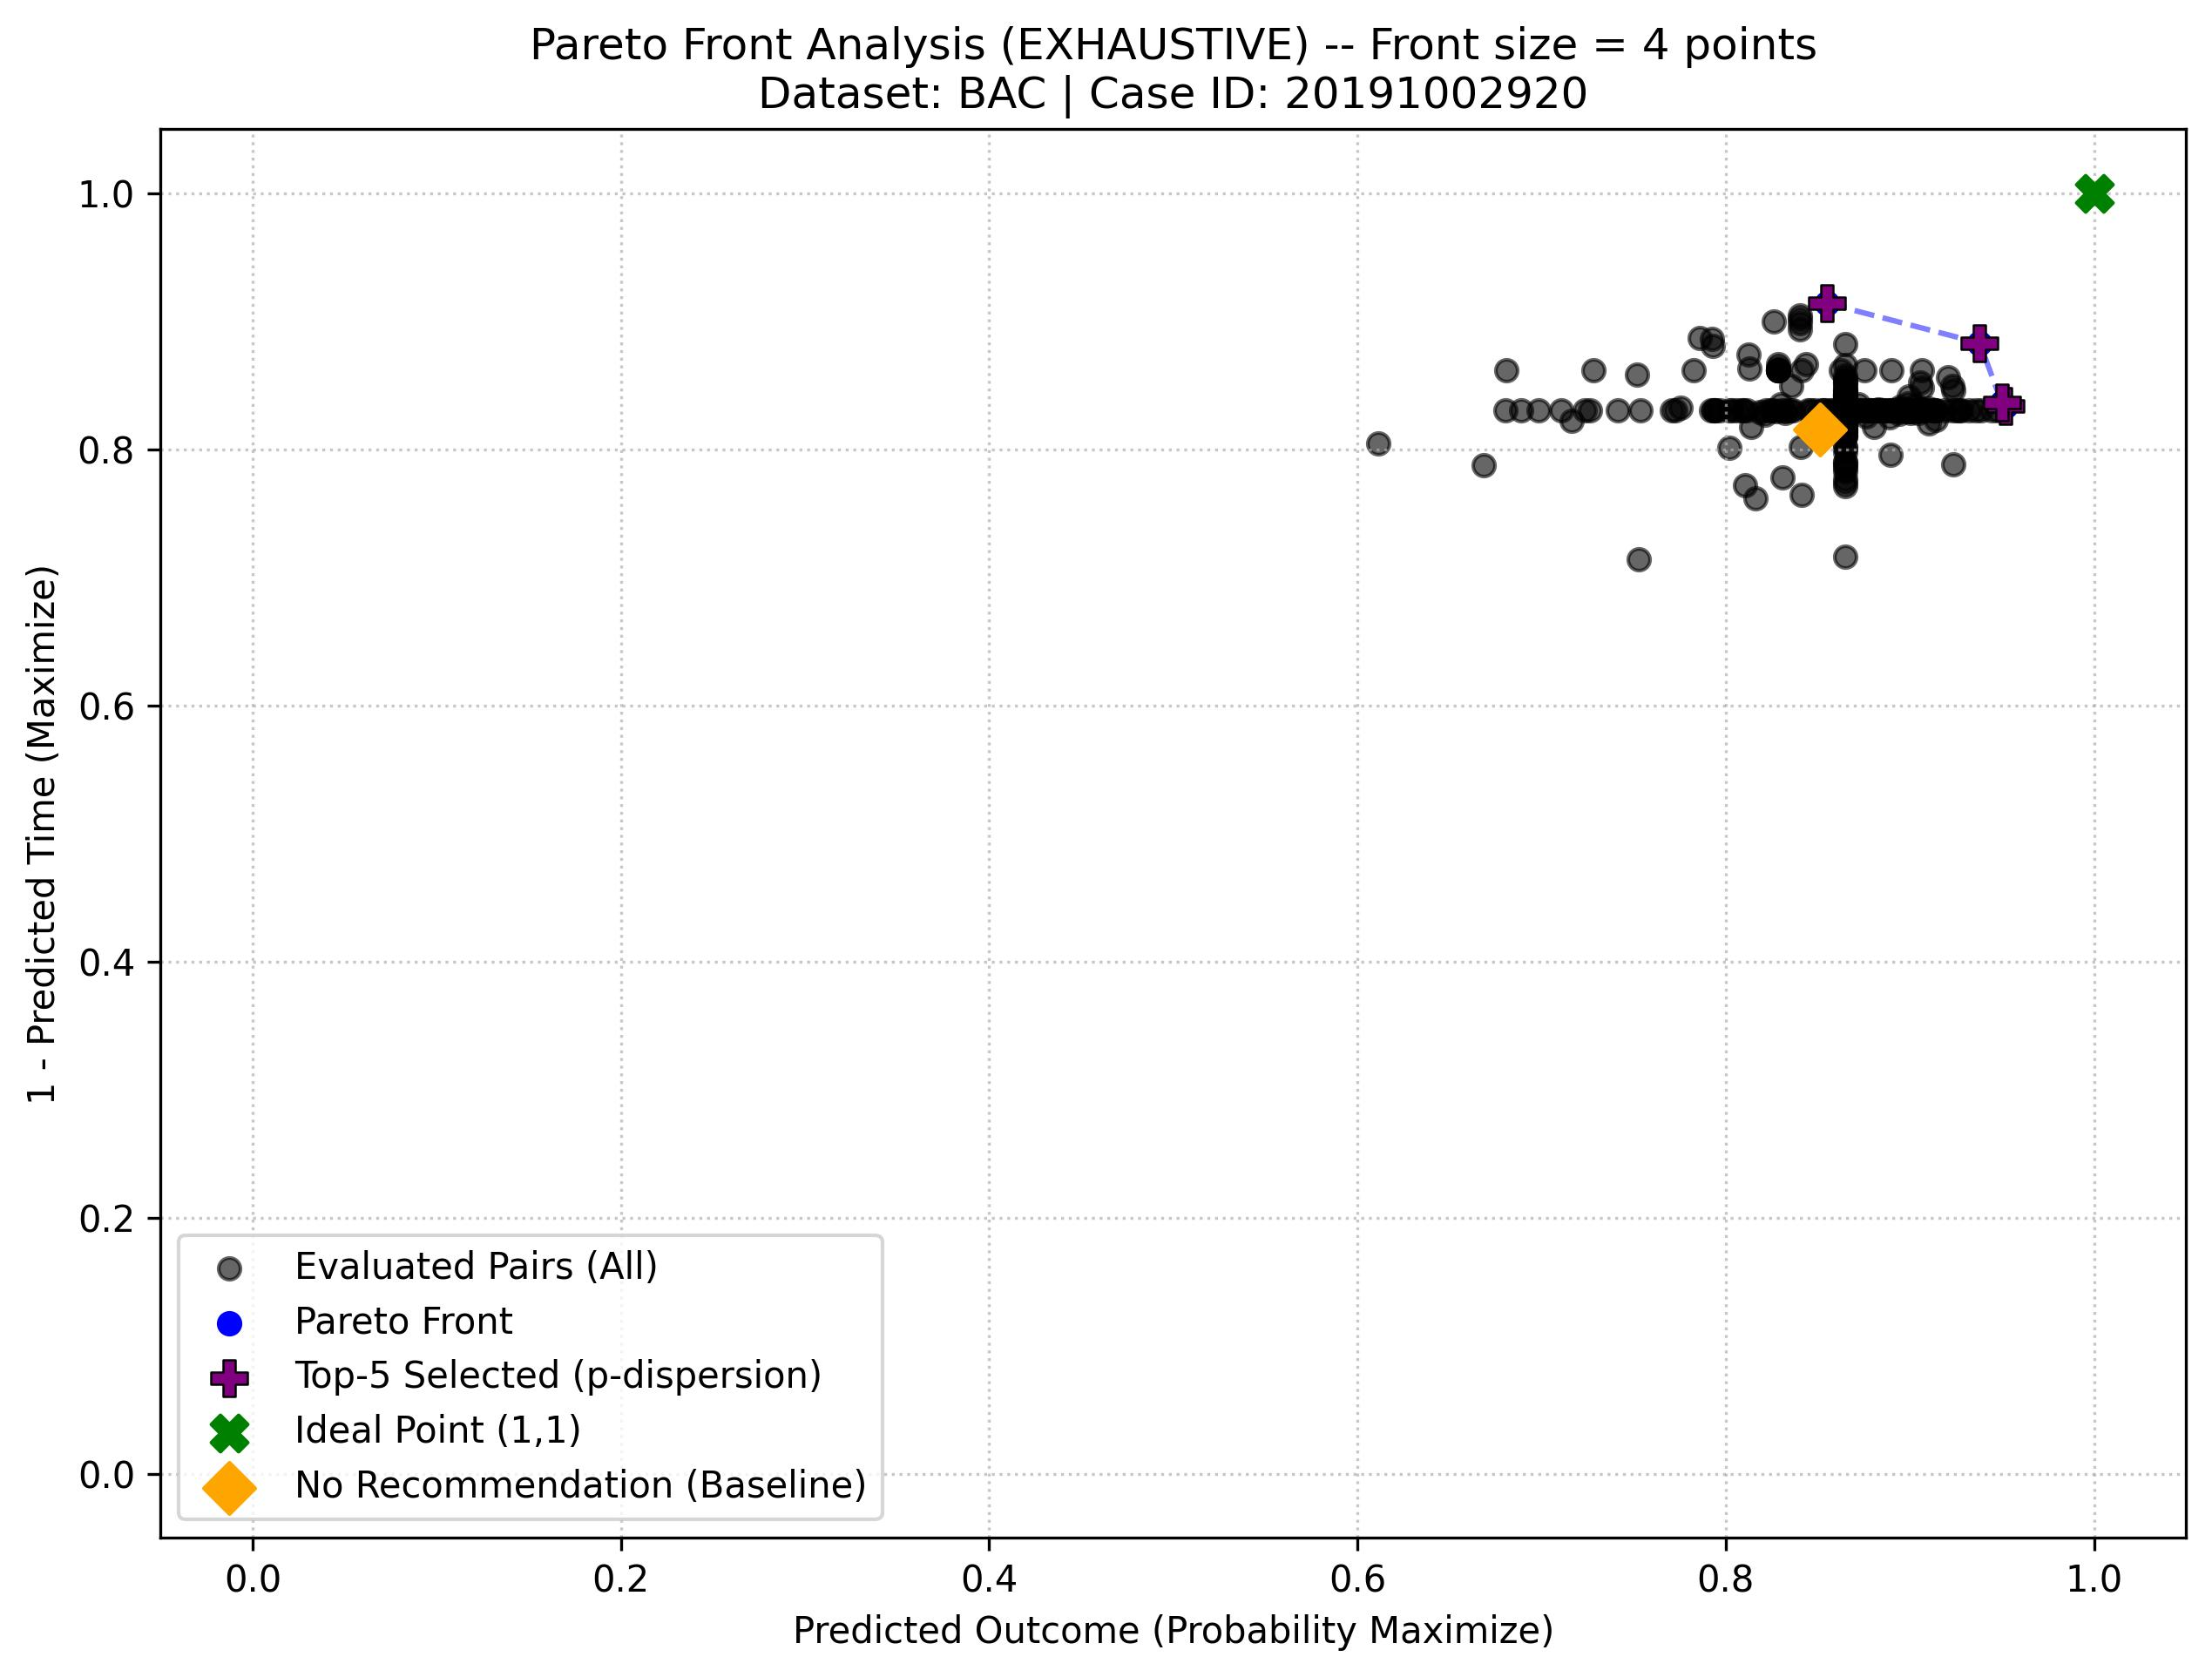
\includegraphics[width=1.03\linewidth]{multi_obj/pareto_fronts/pareto_front_size_examples/pareto_BAC_frontsize_4_20191002920.jpg}
    \end{minipage}

\end{frame}

\begin{frame}{Experimental Results: Pareto Fronts Cardinality examples (BAC)}
    \centering

    \begin{minipage}{0.48\textwidth}
        \centering
        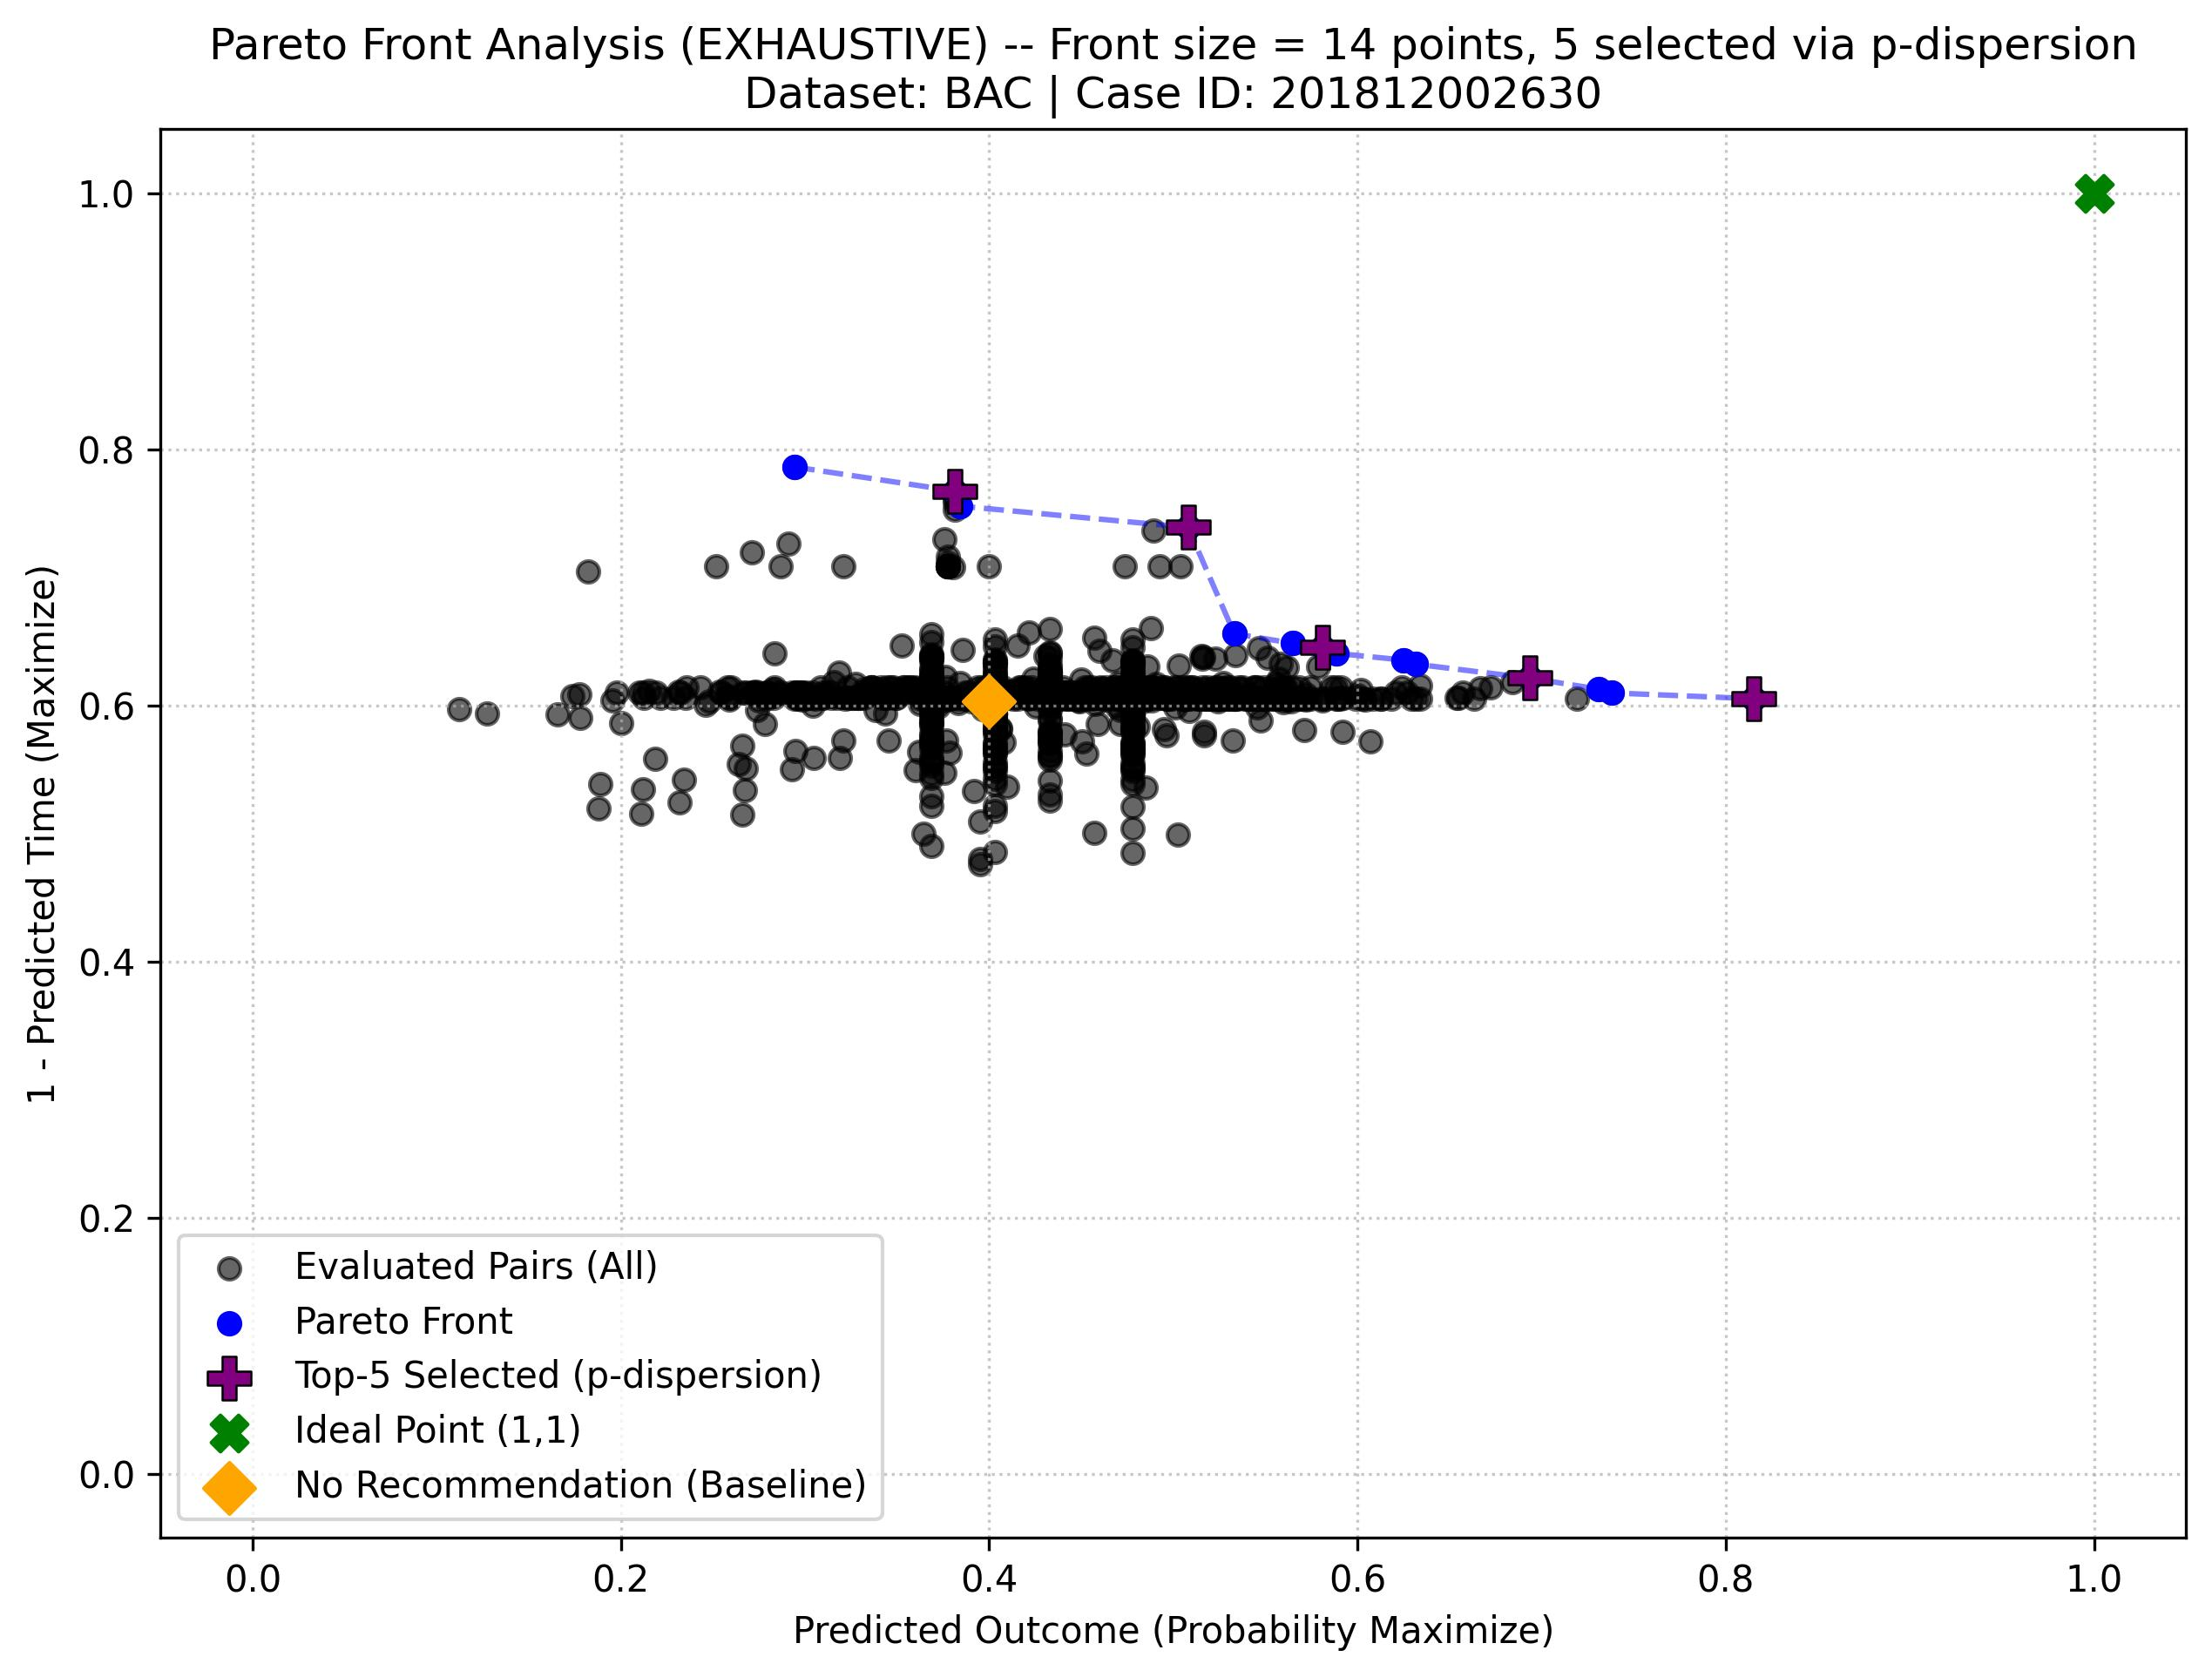
\includegraphics[width=1.03\linewidth]{multi_obj/pareto_fronts/pareto_front_size_examples/pareto_BAC_frontsize_5_201812002630.jpg}
    \end{minipage}


\end{frame}

\section{Evaluation}

\begin{frame}[plain,c]
    \centering
    \color{Darkcandyapplered}
    \Huge\textbf{Evaluation}
\end{frame}

\begin{frame}{Petri Net Discovery}
  \footnotesize
  \begin{itemize}
    \item \textbf{Requirement:} every recommendation of the recommender must be
      \alert{applicable} in the simulation, so the net must replay the whole log
      (\alert{fitness $= 1$}) --- without collapsing into a flower model (low precision).
    \item \textbf{Net used:} the \textbf{directly-follows graph} of the \emph{entire} event log,
      converted into a Petri net (pm4py, ``activity defines place''):
      \begin{itemize}
        \item one place per activity, meaning ``the last activity executed was $X$'';
        \item one transition per step $X \rightarrow Y$ observed in the log, plus start and end.
      \end{itemize}
    \item \textbf{Why it guarantees applicability:} after a prefix ending with $X$, the
      recommender only proposes activities $Y$ that followed a window ending with $X$ in the
      training log, i.e.\ steps $X \rightarrow Y$ of the graph, always enabled in the place $X$.
    \item \textbf{Price:} no concurrency and no long-range constraints (only the last activity
      is remembered) $\Rightarrow$ lower precision than Split Miner.
    \item Before: \textbf{Split Miner}, $(\varepsilon, \eta)$ tuned with \textbf{Optuna} for the best
      F-score: fitness $< 1$, many recommendations \alert{unreachable} (83\% of rank 1 on BPI12).
  \end{itemize}
  {\scriptsize Script: \texttt{discovery/petri\_net\_discovery\_fitness1.py}.}
\end{frame}

\begin{frame}{Petri Net Discovery: Candidate Nets}
  \small
  Token-based replay on the entire event log. Fit.\ tr.: share of traces replayed with no
  deviation. The Inductive Miner is run with noise threshold $0$ (fitness $1$ by construction).
  \begin{center}\setlength{\tabcolsep}{4pt}
  \begin{tabular}{l rrr rr rr}
    \toprule
     & \multicolumn{3}{c}{Split Miner (best F-score)} & \multicolumn{2}{c}{Inductive Miner}
     & \multicolumn{2}{c}{\alert{Directly-follows}} \\
    \cmidrule(lr){2-4}\cmidrule(lr){5-6}\cmidrule(lr){7-8}
    Dataset & Fitness & Fit.\ tr. & Prec. & Fitness & Prec. & Fitness & Prec. \\
    \midrule
    BAC          & 0.992 & 90.3\% & 0.911 & 1.000 & 0.504 & 1.000 & 0.866 \\
    BPI12        & 0.953 &  3.8\% & 0.678 & 1.000 & 0.226 & 1.000 & 0.877 \\
    bpi17-before & 0.982 & 68.3\% & 0.835 & 1.000 & 0.275 & 1.000 & 0.556 \\
    bpi17-after  & 0.974 & 57.6\% & 0.849 & 1.000 & 0.266 & 1.000 & 0.566 \\
    \bottomrule
  \end{tabular}
  \end{center}
  \scriptsize
  \begin{itemize}
    \item \textbf{Inductive Miner:} handles concurrency in principle, but to reach fitness 1 on
      these loop-rich logs it falls back to flower-like blocks (many silent transitions, e.g.\
      54 against 7 on BAC): \alert{precision about halved} on BAC.
    \item \textbf{Directly-follows:} fitness 1 on every dataset (100\% of the traces), the
      highest precision among the fitness-1 nets; used by the simulator.
      Source: \texttt{discovery/petri\_net\_quality.csv}. Split Miner and Inductive Miner: BPI12/bpi17 logs \emph{with} \texttt{W\_}, not recomputed.
  \end{itemize}
\end{frame}

\begin{frame}{Simulator Calibration}
    \begin{itemize}
        \item Given the discovered Petri net and the event log, the \textbf{ProSiT} simulation engine learns its stochastic parameters:
        \begin{itemize}
            \item resource pools and availability,
            \item transition (routing) probabilities,
            \item resource calendars,
            \item execution, waiting, and arrival time distributions.
        \end{itemize}
        \item These parameters fully configure the simulator, enabling it to replay and extend running cases stochastically, consistently with historical process behavior.
    \end{itemize}
\end{frame}

\begin{frame}{Baseline Simulation}
    \begin{itemize}
        \item For every test case, the simulator is given only the observed \textbf{prefix} (no recommendation) and left free to complete the case on its own.
        \item This reproduces how the process would continue \textit{without} any recommendation, and serves as the reference point for evaluating the recommendation methods.
        \item Because the simulator is stochastic, \textbf{10 independent simulation runs} are performed per case to account for variability.
    \end{itemize}
\end{frame}

\begin{frame}{Method Simulation: Prefix Replay \& Strict Recommendation}
  \footnotesize
    \begin{itemize}
        \item For the recommendation method (\textbf{exhaustive}), the same prefix is simulated again, but the simulator additionally receives the recommended (activity, resource) pair as the \textbf{next} event; it is then free to complete the case from there.
        \item \textbf{Prefix replay:} the historical prefix is replayed on the Petri net
          \alert{exactly} (token replay); alignments are used only as a fallback for the
          prefixes the net cannot replay (non-fitting prefixes).
        \item \textbf{Strict recommendation:} the recommended activity must be the
          \alert{next visible step} --- enabled in the reconstructed marking, or reachable
          through \emph{silent} transitions only. Reaching it through other visible
          activities is not allowed: they would happen with no event, time or resource.
        \item Otherwise the recommendation is \alert{unreachable}: the case continues
          without it and that run is excluded from the evaluation. Unreachability depends
          only on the replayed prefix, so it holds in all runs of that case.
        \item Each test case has up to $k$ diverse recommendations, so this is repeated
          \textbf{10 runs $\times$ $k$ ranks} per case.
    \end{itemize}
\end{frame}

\begin{frame}{Simulation: How Many Recommendations Can Be Applied}
  \footnotesize
  Test cases \alert{simulated} at each rank (with a recommendation at that rank), $\gamma = 0.5$, $k = 5$,
  10 runs. All of them are \alert{usable}: the recommendation is applied in every run.
  \begin{center}\setlength{\tabcolsep}{5pt}
  \begin{tabular}{lrrrrrr}
    \toprule
    Dataset (test cases) & Rank 1 & Rank 2 & Rank 3 & Rank 4 & Rank 5 & \shortstack{R-1 usable,\\ \% of test} \\
    \midrule
    BAC (1876)          & 1871 &  381 &   41 &    0 &   0 &  99.7\% \\
    BPI12 (623)         &  601 &  215 &  149 &   13 &   0 &  96.5\% \\
    bpi17-before (1218) & 1168 &  228 &   34 &    6 &   0 &  95.9\% \\
    bpi17-after (1840)  & 1799 &  490 &   56 &    0 &   0 &  97.8\% \\
    \bottomrule
  \end{tabular}
  \end{center}
  \begin{itemize}
    \item \alert{No unreachable recommendation} in any run or rank, no non-fitting prefix, no truncated case:
      the fitness-1 directly-follows net replays every prefix and allows every step of the log.
    \item Before, with the Split Miner net: only 17\% of rank 1 usable on BPI12, 66\% on BAC.
    \item Most frequent rank-1 recommendations: BAC \emph{Pending Liquidation Request} (34\%); BPI12
      \texttt{O\_SENT\_BACK} (81\%); bpi17 \texttt{A\_Validating} (89\% before, 73\% after).
  \end{itemize}
  {\scriptsize Source: \texttt{4\_simulation\_summary\_<case>.txt}, \texttt{3\_recommendations\_summary.csv}.}
\end{frame}

\begin{frame}{Open Question: Recommending Customer Events}
  \small
  \begin{itemize}
    \item With the fitness-1 net every recommendation can be applied in the simulation (previous slide).
    \item But the most frequent ones (\texttt{O\_SENT\_BACK}, 81\% of rank 1 on BPI12; \texttt{A\_Validating},
      73--89\% on bpi17) are events that follow a \alert{customer} action, not a bank activity: the simulator
      executes them, the bank could not simply do so.
    \item The recommender proposes what followed the same recent history in the training log (transition
      system, window 5), and it is deliberately kept independent of the simulator.
    \item \textbf{In production}, options:
      \begin{enumerate}
        \item recommend only activities the bank can execute (no customer events);
        \item fall back to the next point of the Pareto front, or to no recommendation.
      \end{enumerate}
  \end{itemize}
\end{frame}

\begin{frame}{Result Computation \& Validation}
    \begin{itemize}
        \item For each case, the \textbf{outcome} and \textbf{remaining time} are averaged over the 10 simulation runs, separately for the baseline and for each recommendation method/rank.
        \item The same quantities are also computed \textit{without simulating}, directly from the \textbf{offline-phase} CatBoost regressor and classifier, applied to the prefix with the recommended next step and with \texttt{\_\_NO\_NEXT\_\_} (the same ``no recommendation'' baseline used by the confidence filter); the remaining time is the expected value in days (truncated log-normal mean), as in the recommender.
        \item Comparing simulated vs.\ predicted values makes it possible to assess how well the offline predictive models agree with the actual stochastic behavior reproduced by the simulator.
    \end{itemize}
\end{frame}

\begin{frame}{Experimental Results: Predicted vs.\ Simulated (BAC)}
    \centering

    \begin{minipage}{0.45\textwidth}
        \centering
        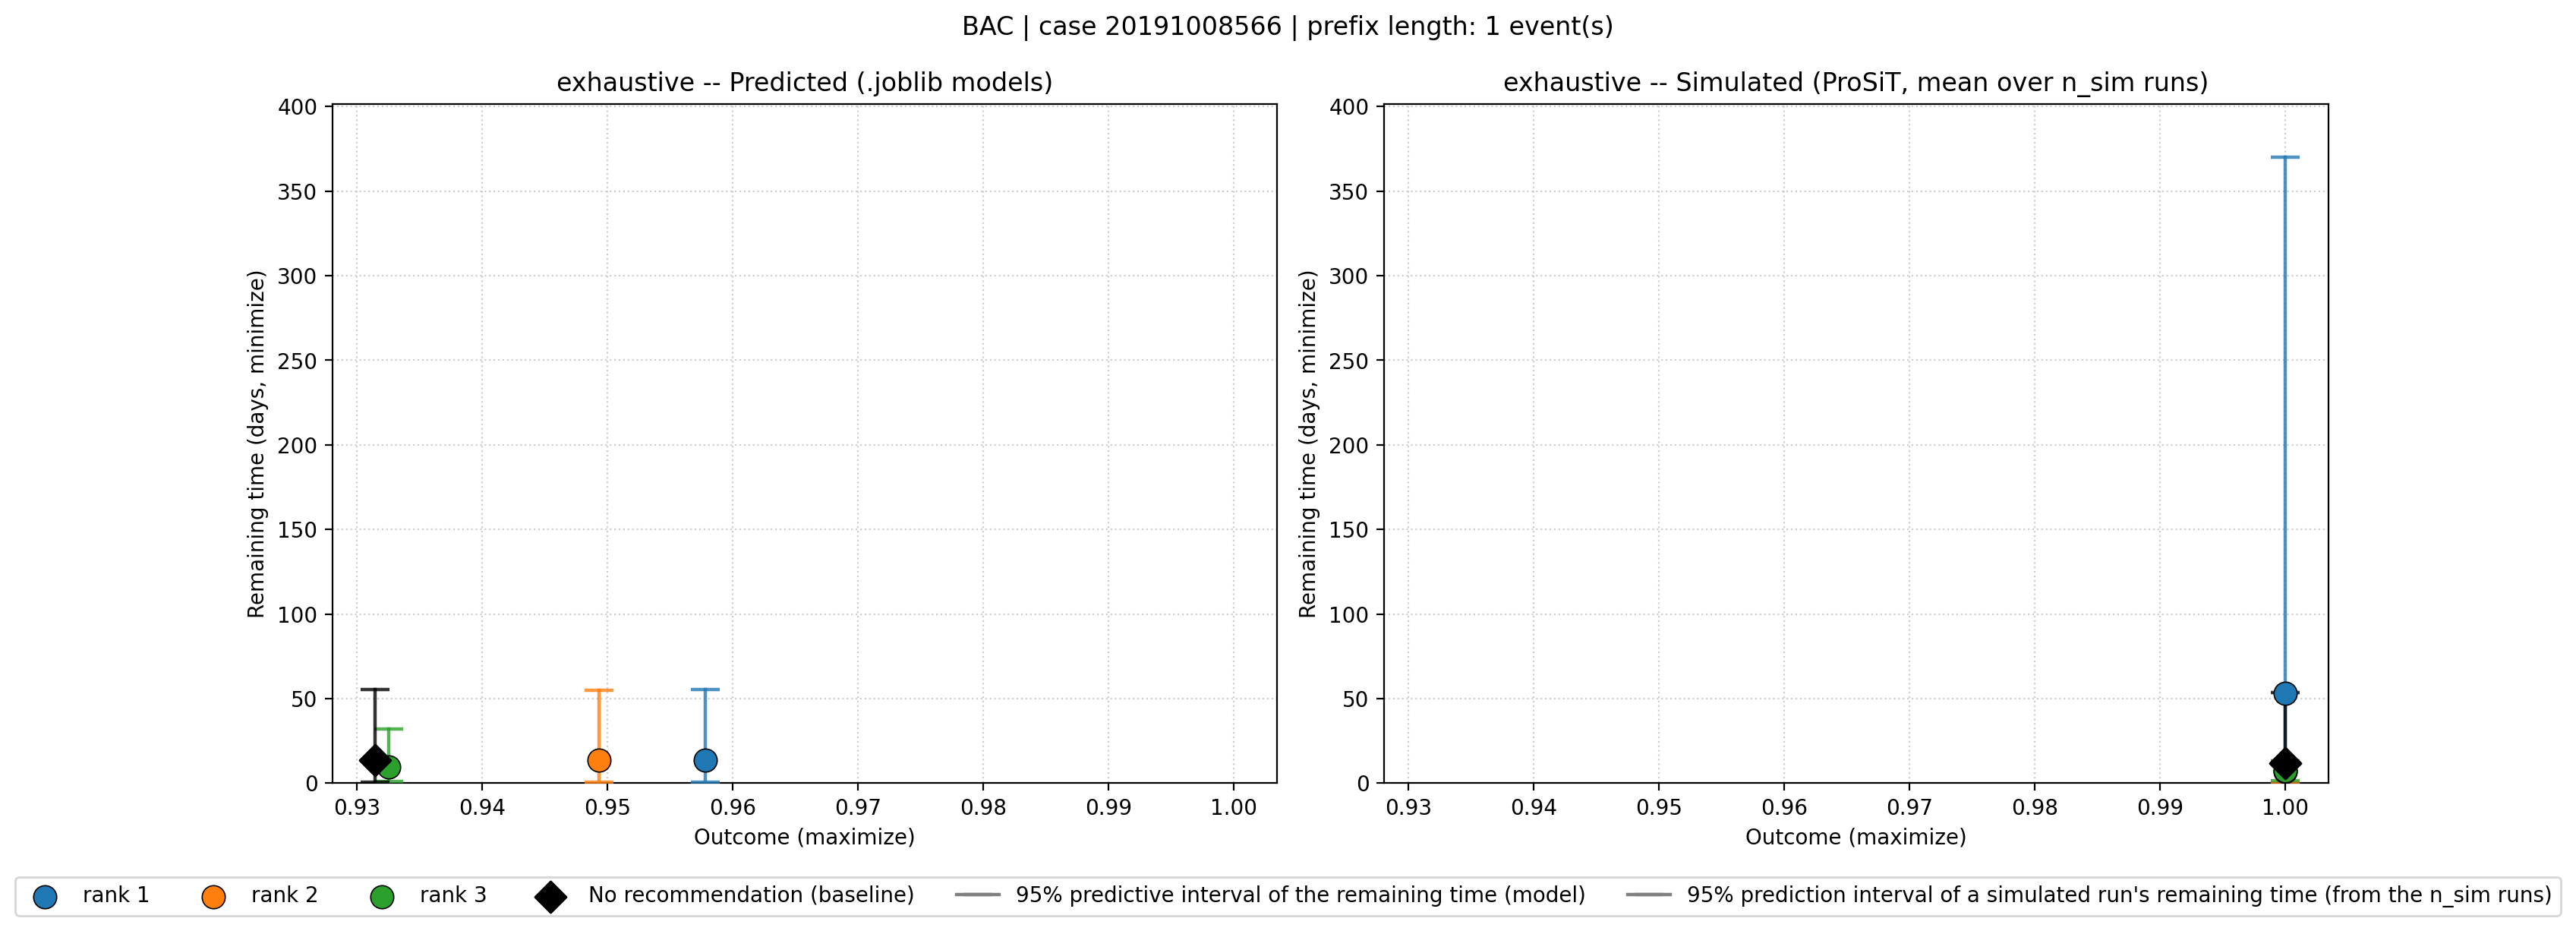
\includegraphics[width=\linewidth]{multi_obj/pareto_fronts/pareto_fronts_predicted_vs_simulated/BAC/BAC_20191008566_exhaustive_predicted_vs_simulated.png}
    \end{minipage}
    \hfill
    \begin{minipage}{0.45\textwidth}
        \centering
        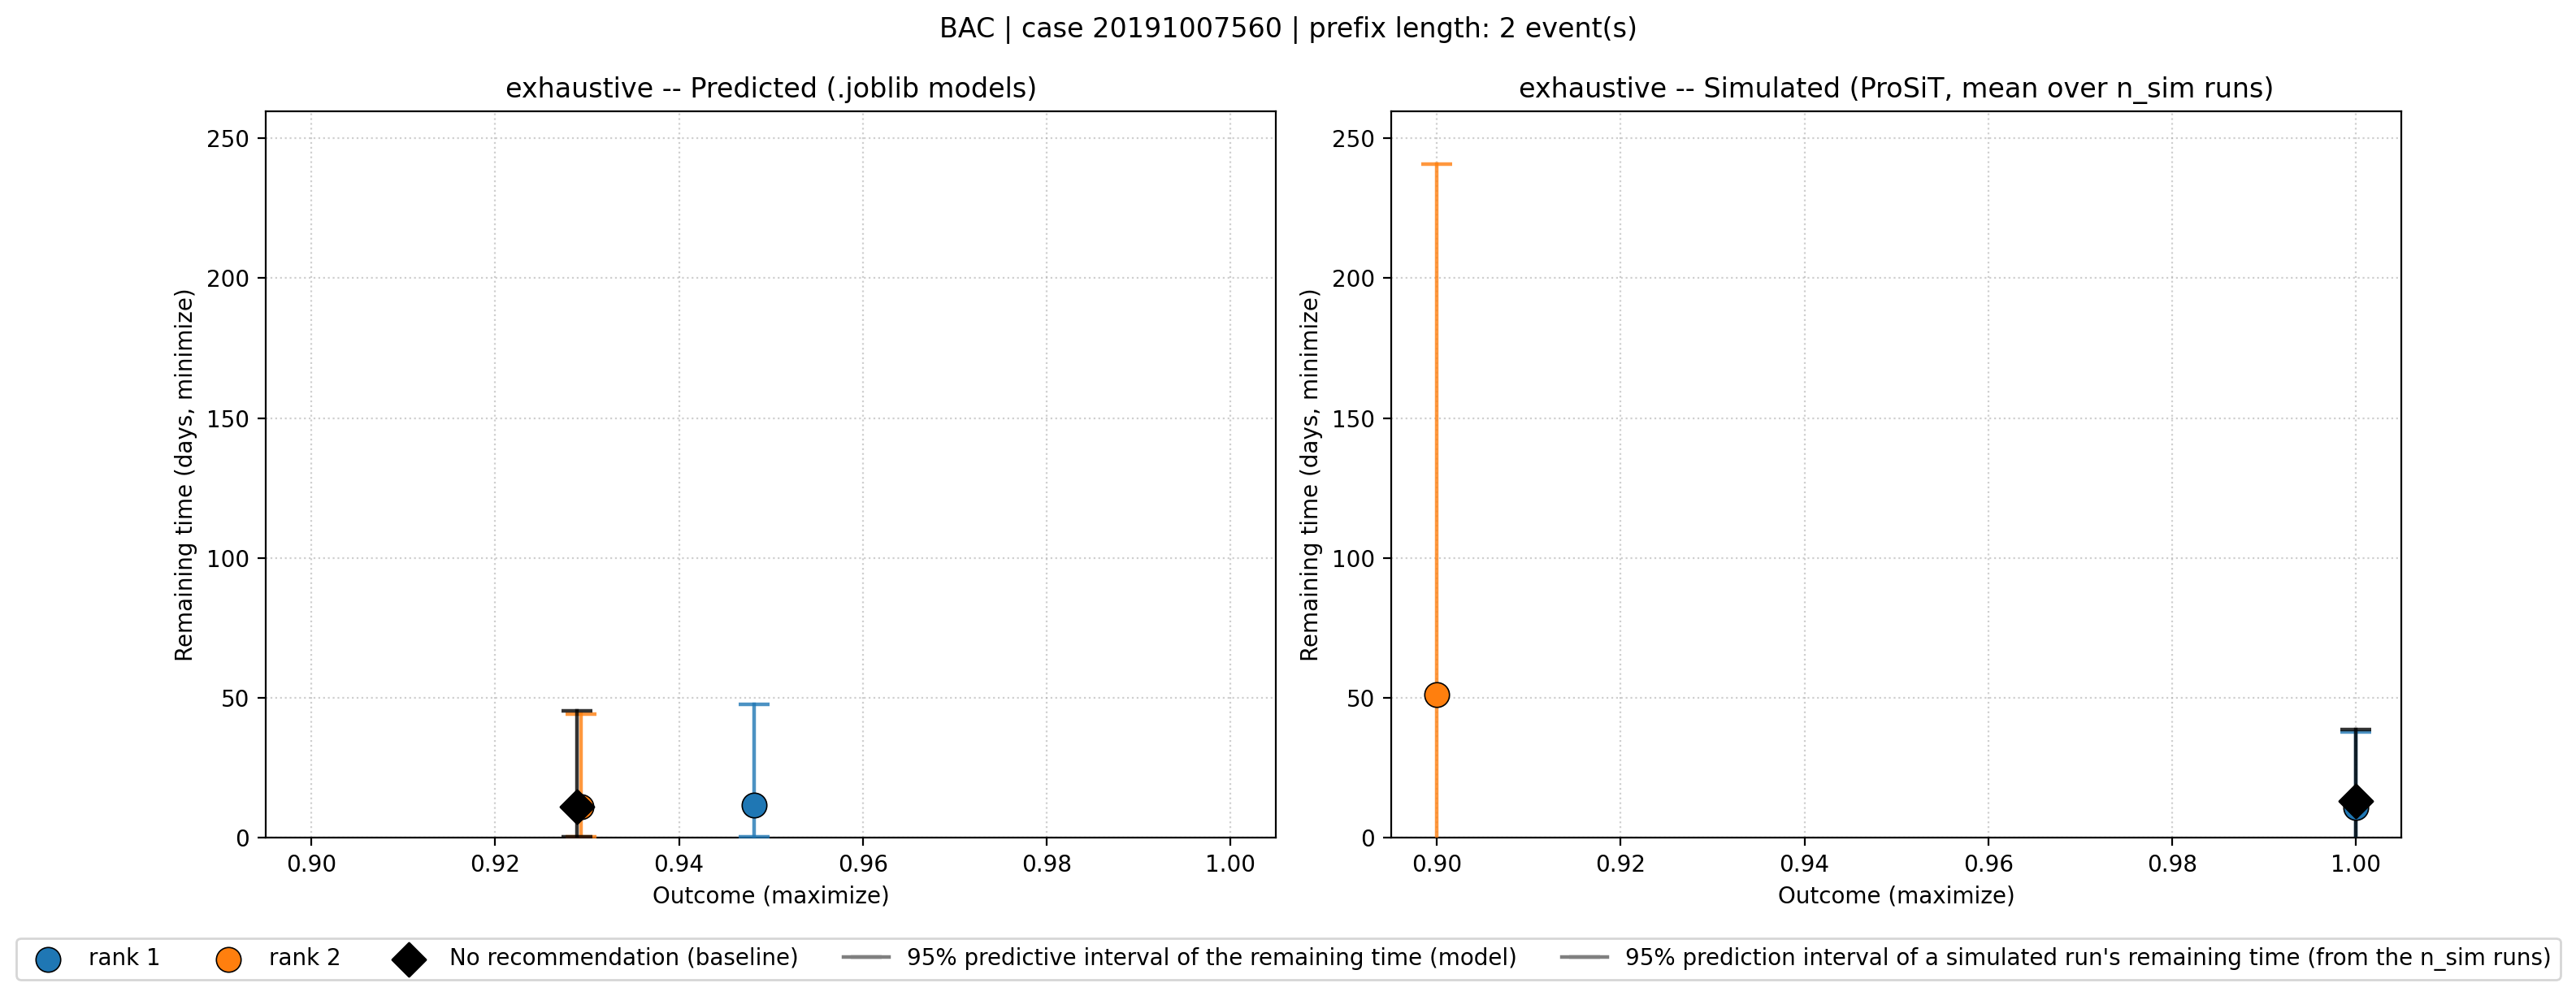
\includegraphics[width=\linewidth]{multi_obj/pareto_fronts/pareto_fronts_predicted_vs_simulated/BAC/BAC_20191007560_exhaustive_predicted_vs_simulated.png}
    \end{minipage}
    \vspace{0.4cm}
    \begin{minipage}{0.45\textwidth}
        \centering
        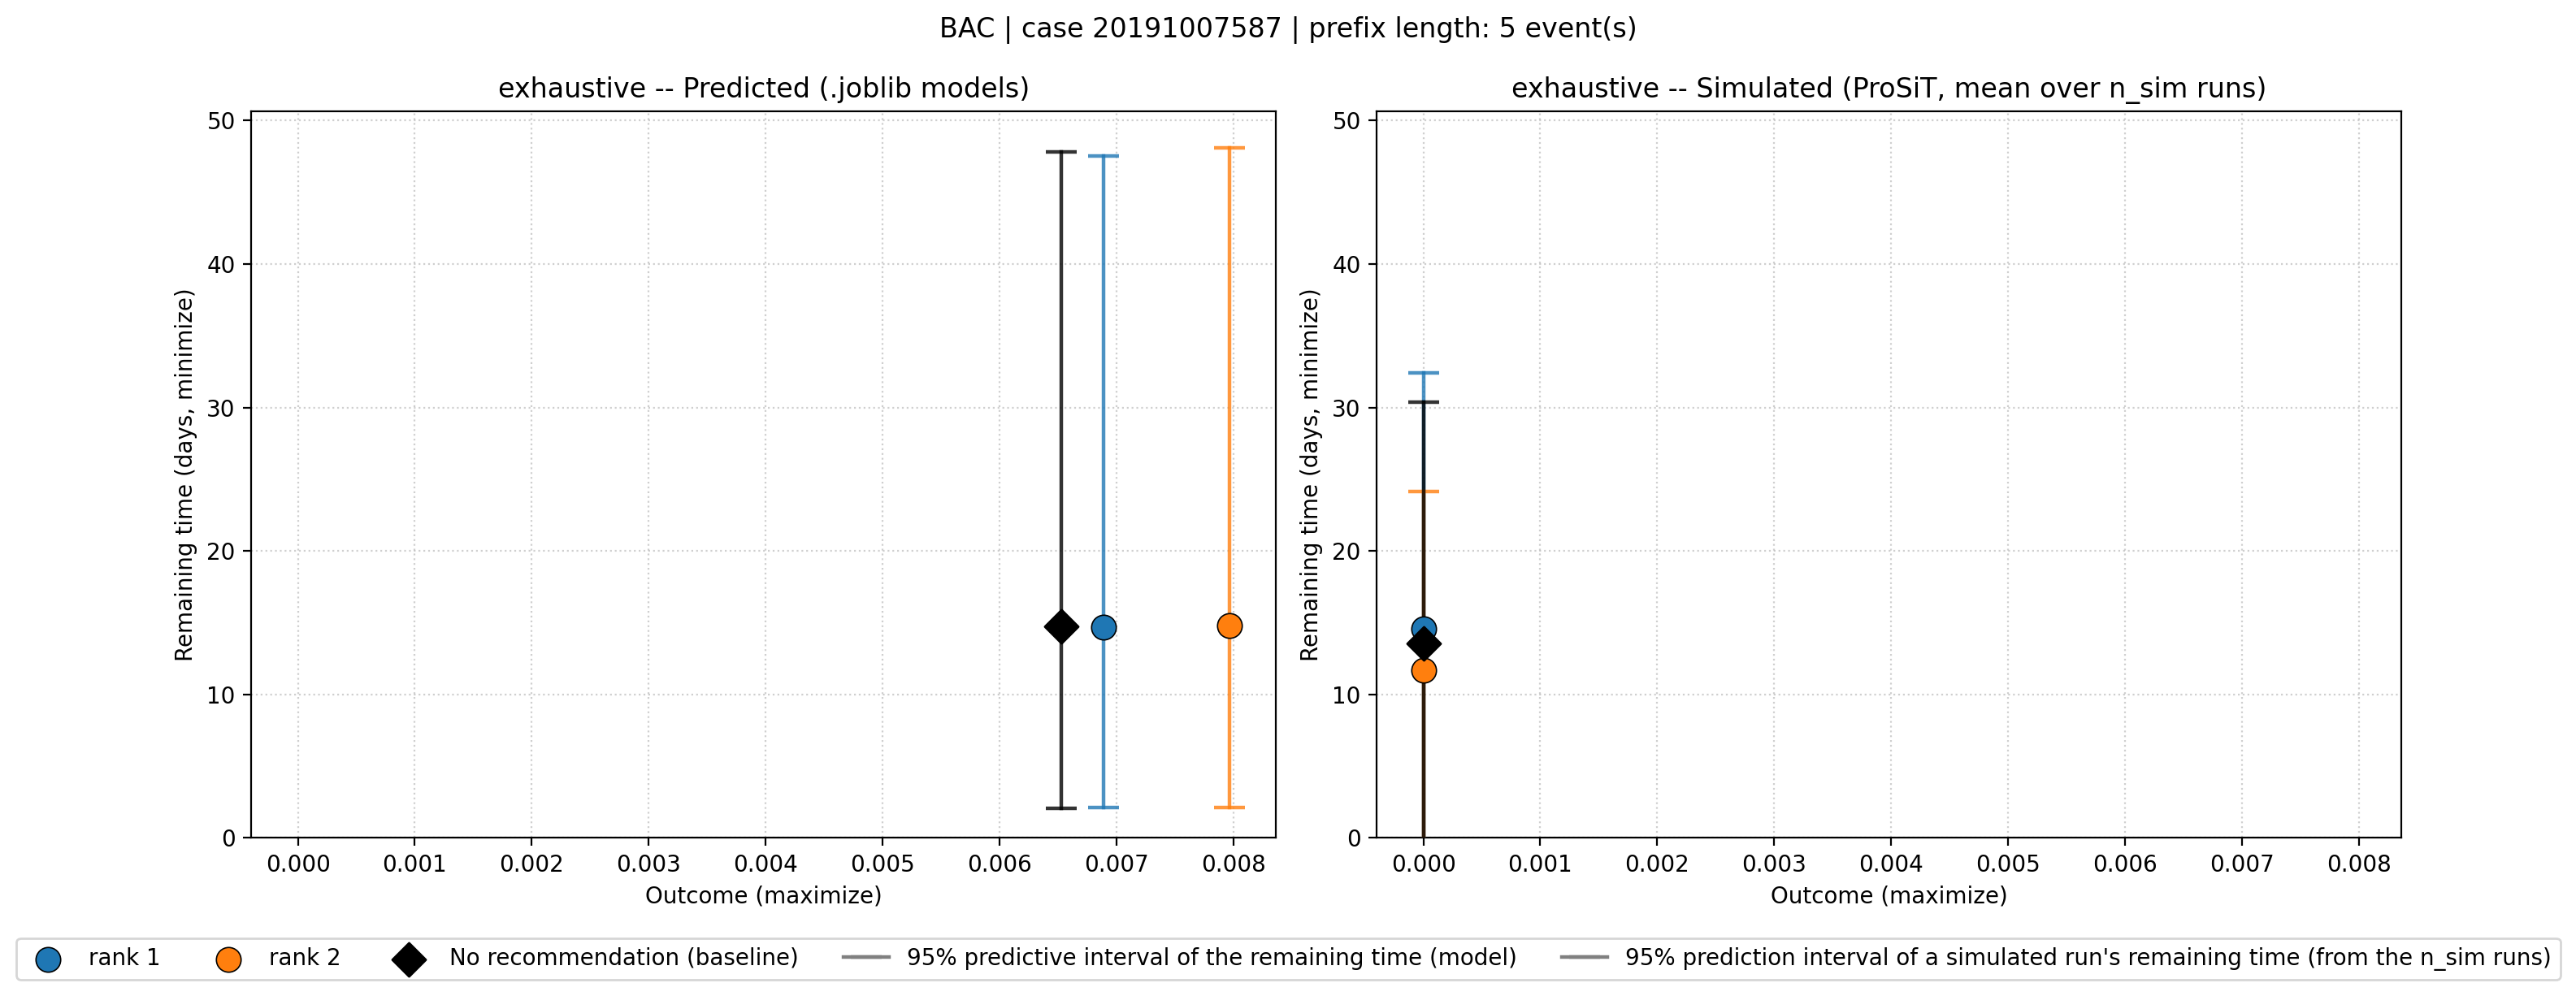
\includegraphics[width=\linewidth]{multi_obj/pareto_fronts/pareto_fronts_predicted_vs_simulated/BAC/BAC_20191007587_exhaustive_predicted_vs_simulated.png}
    \end{minipage}
\end{frame}

\begin{frame}{Experimental Results: Predicted vs.\ Simulated (BPI12)}
    \centering
    \begin{minipage}{0.45\textwidth}
        \centering
        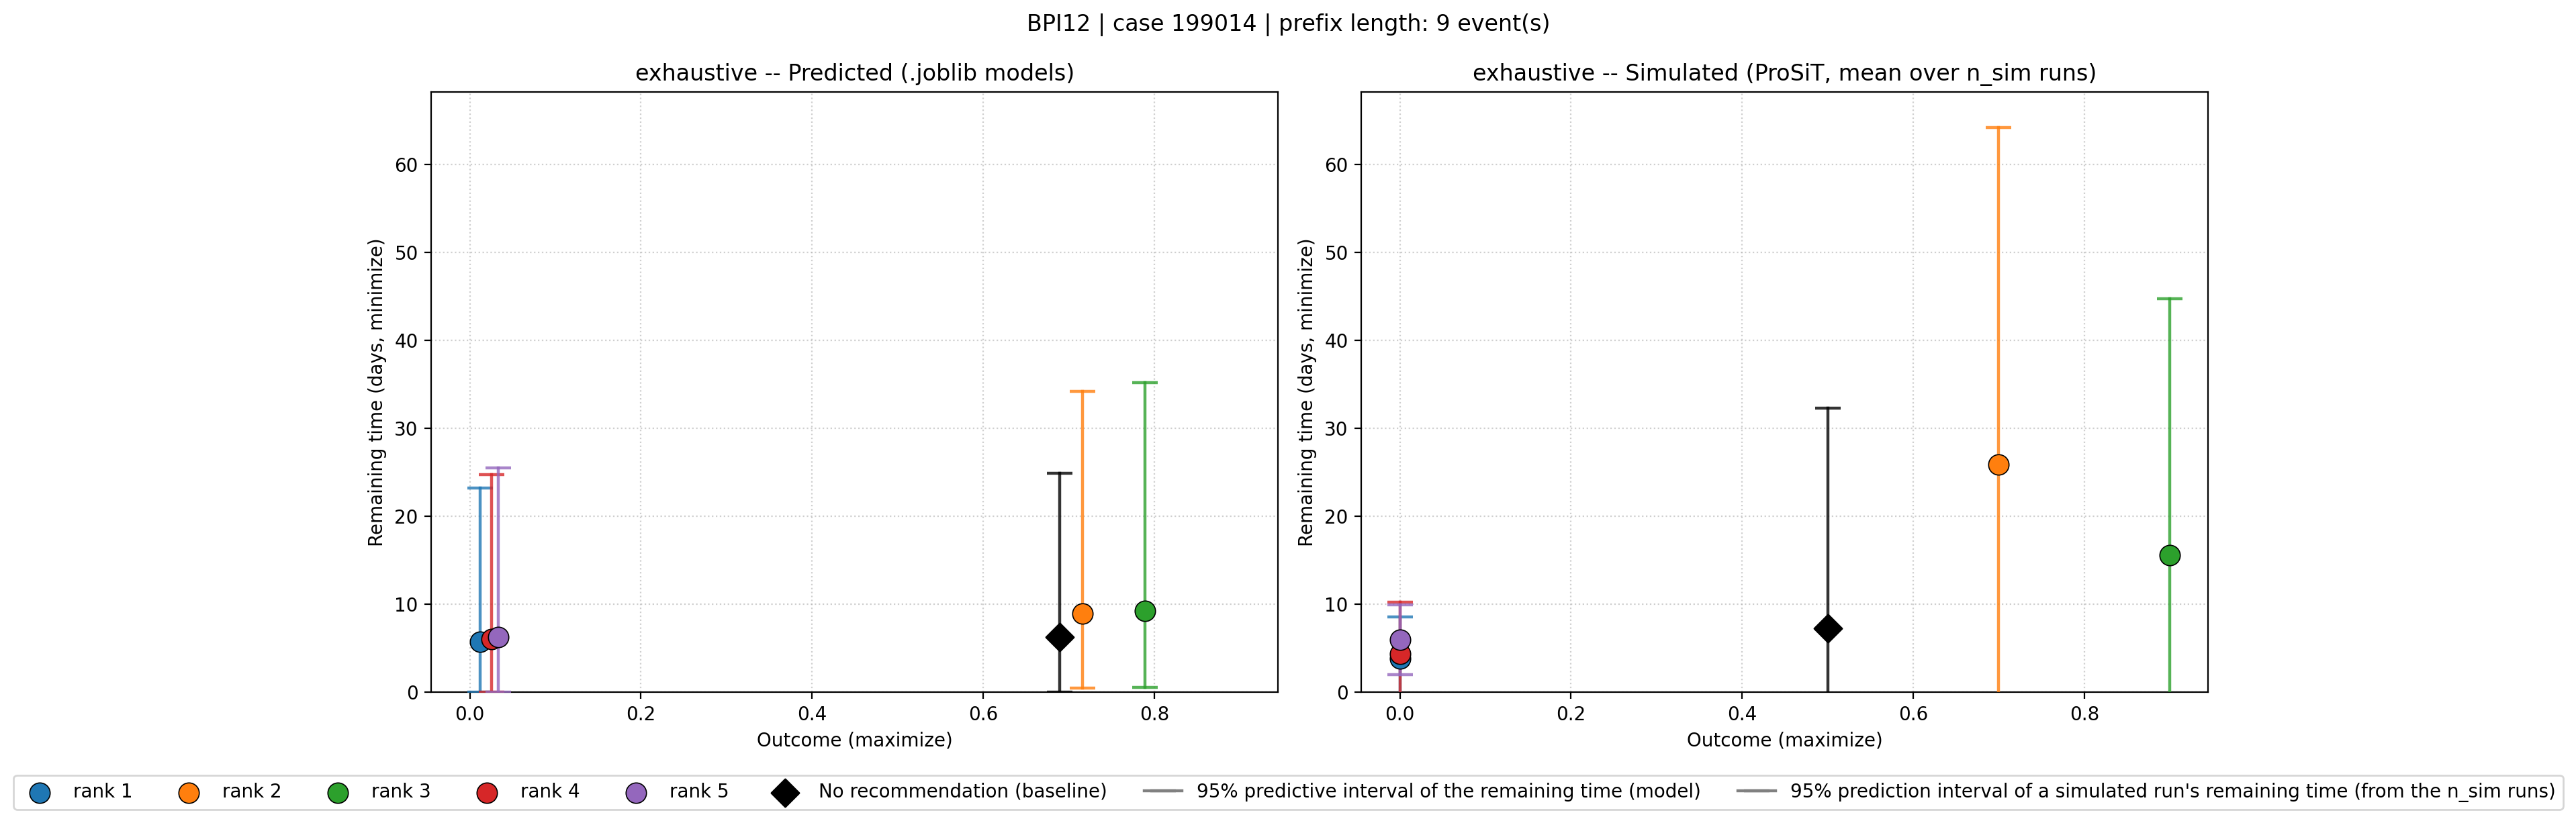
\includegraphics[width=\linewidth]{multi_obj/pareto_fronts/pareto_fronts_predicted_vs_simulated/BPI12/BPI12_199014_exhaustive_predicted_vs_simulated.png}
    \end{minipage}
    \hfill
    \begin{minipage}{0.45\textwidth}
        \centering
        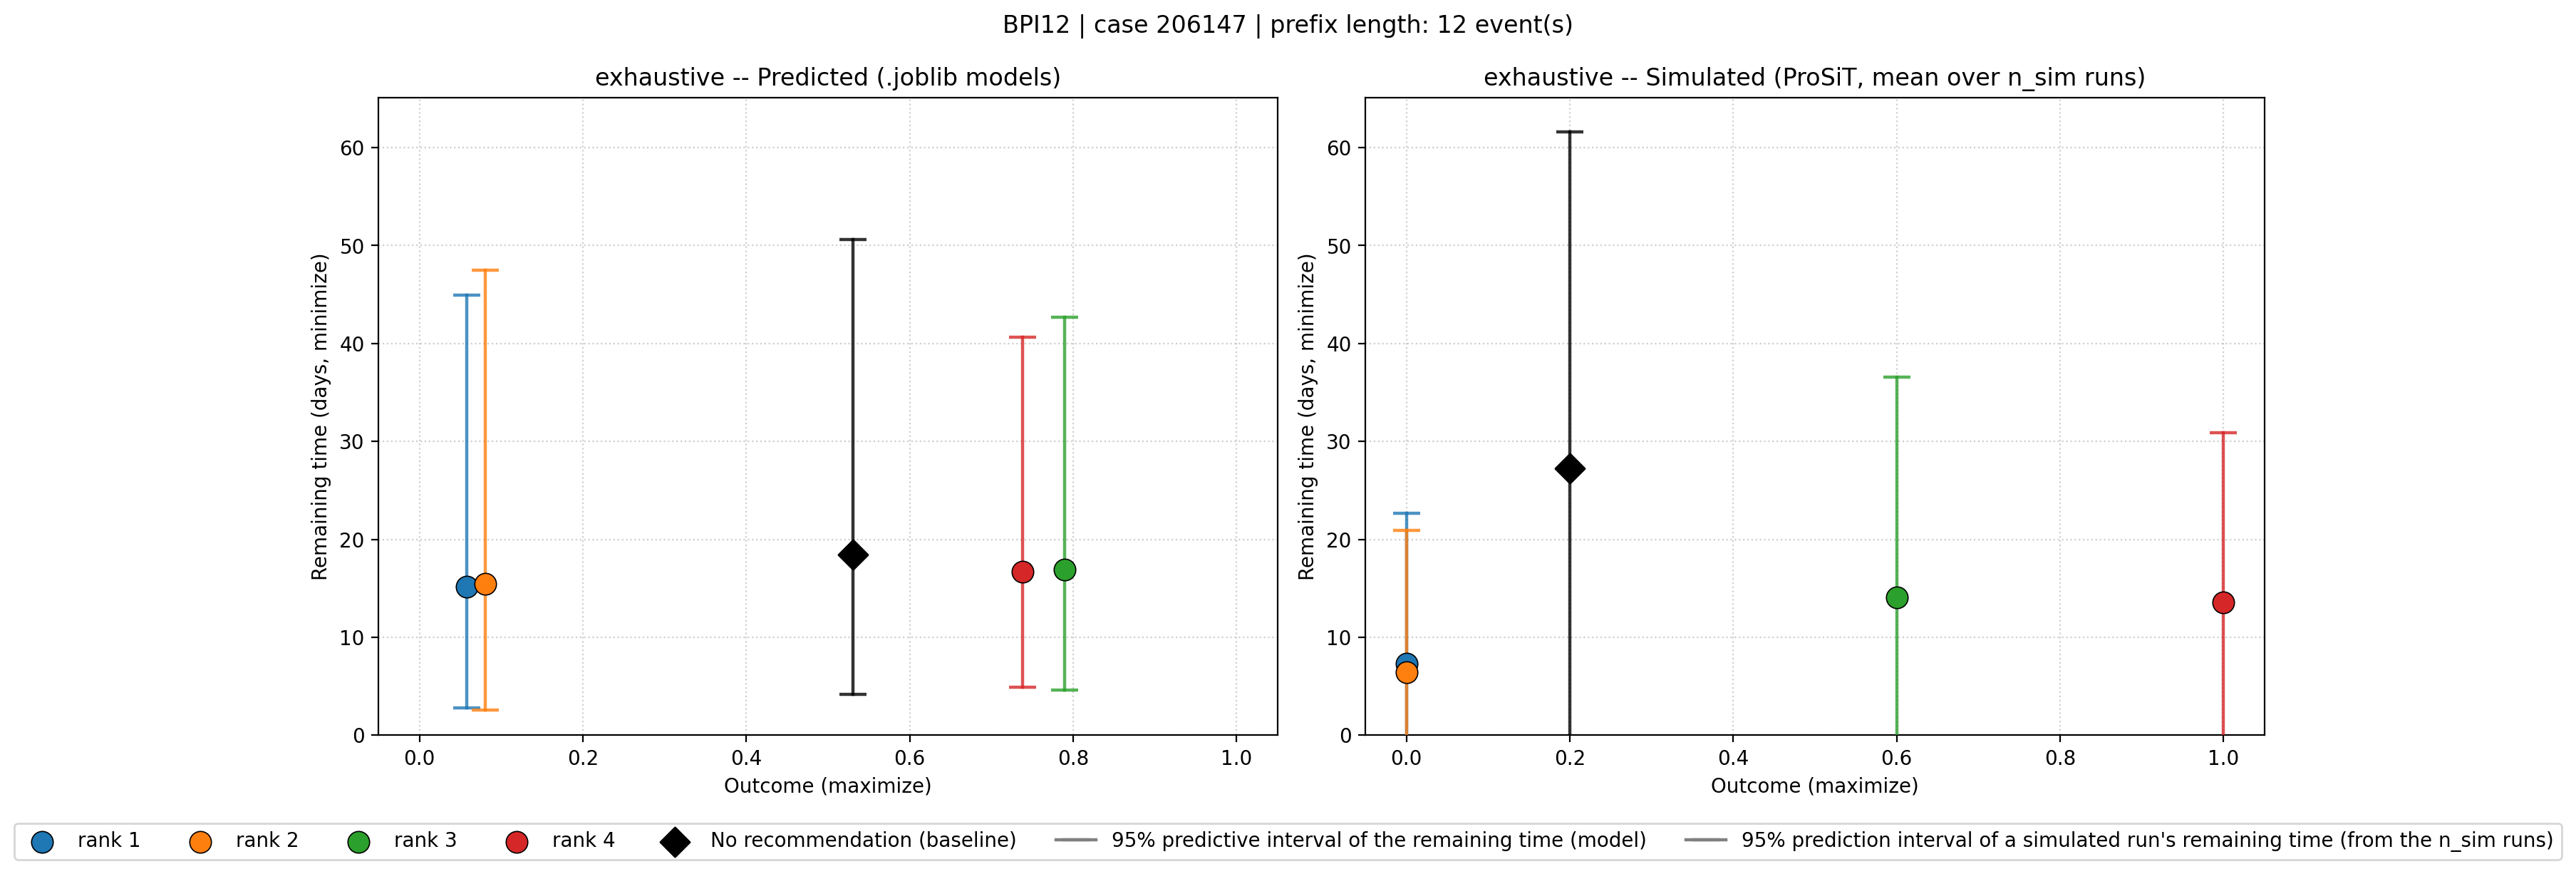
\includegraphics[width=\linewidth]{multi_obj/pareto_fronts/pareto_fronts_predicted_vs_simulated/BPI12/BPI12_206147_exhaustive_predicted_vs_simulated.png}
    \end{minipage}
    \vspace{0.4cm}
    \begin{minipage}{0.45\textwidth}
        \centering
        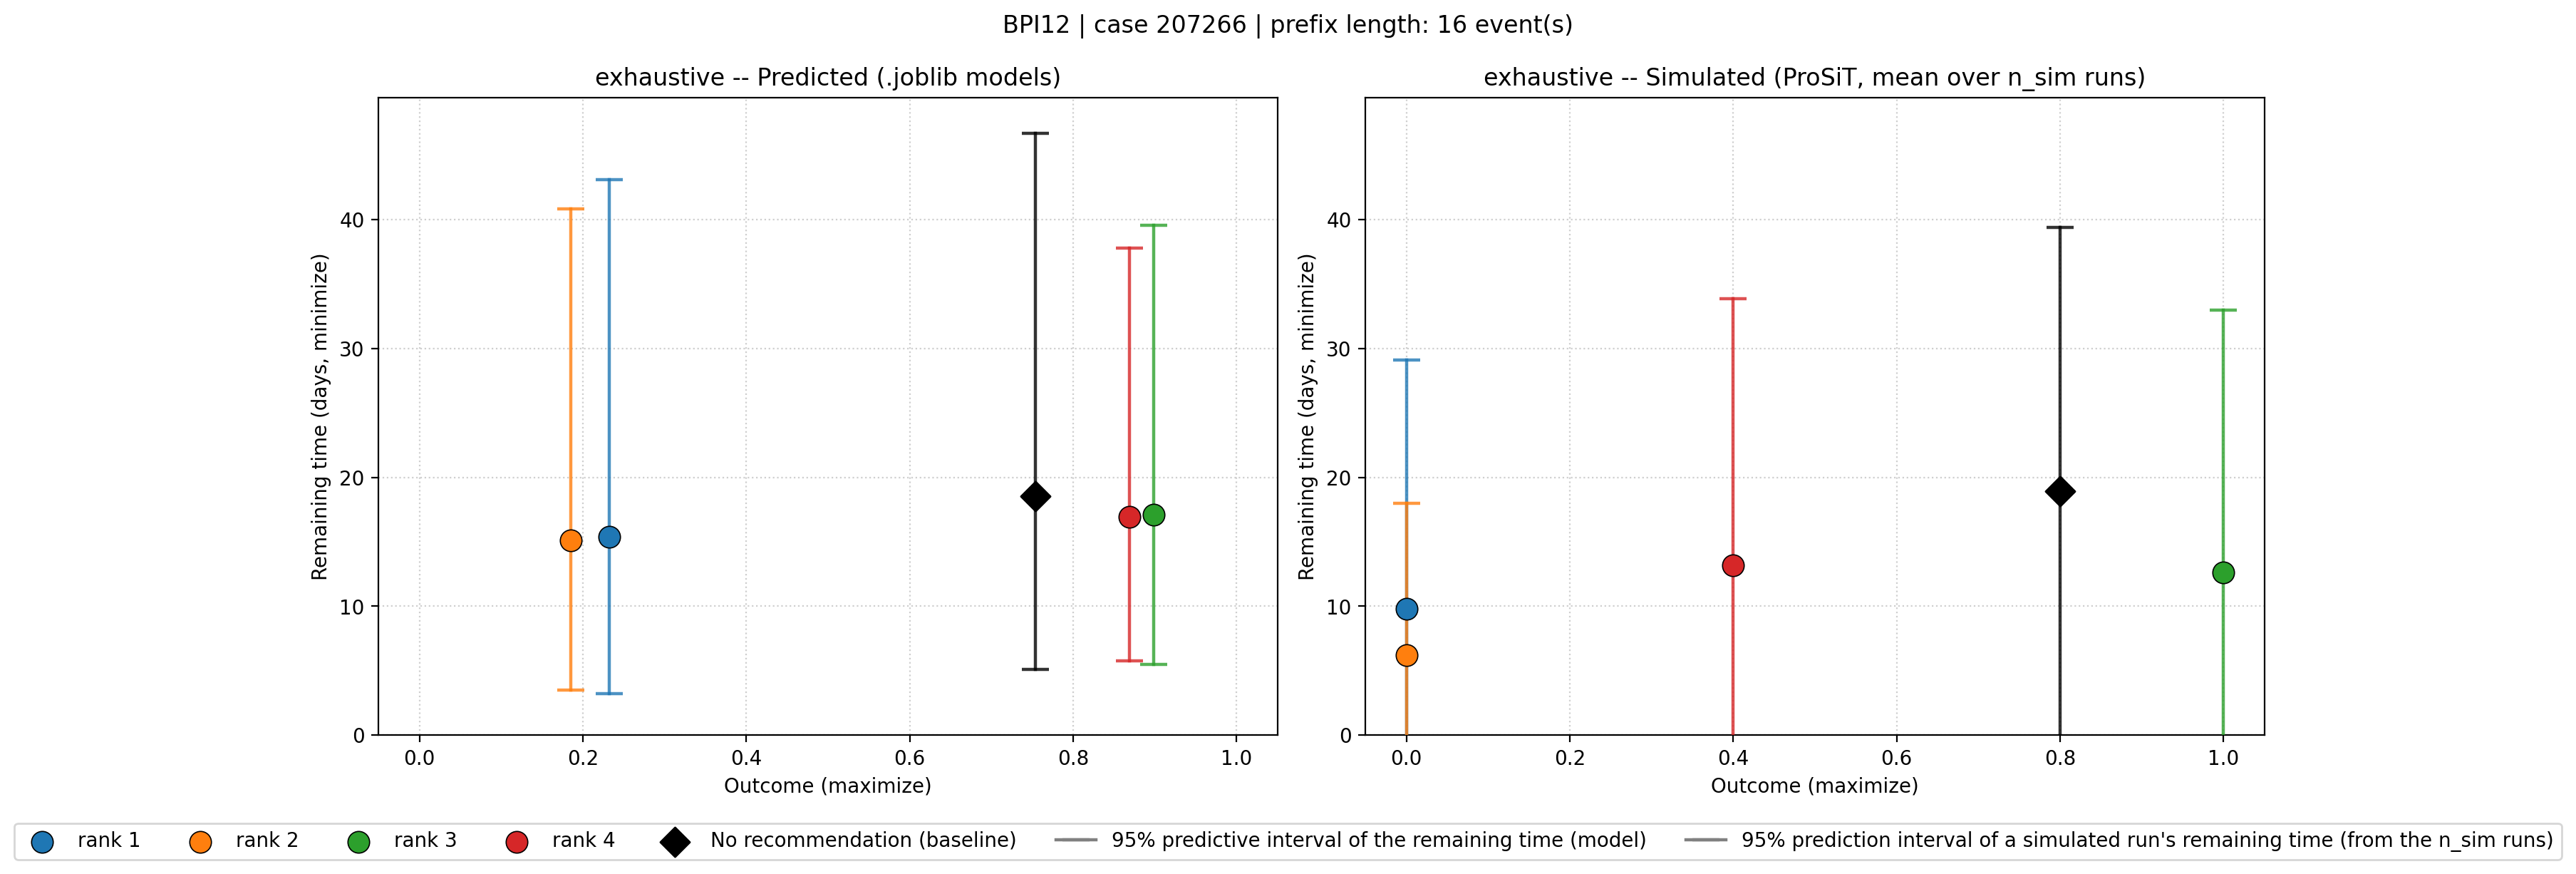
\includegraphics[width=\linewidth]{multi_obj/pareto_fronts/pareto_fronts_predicted_vs_simulated/BPI12/BPI12_207266_exhaustive_predicted_vs_simulated.png}
    \end{minipage}
\end{frame}

\begin{frame}{Experimental Results: Predicted vs.\ Simulated (bpi17 before)}
    \centering
    \begin{minipage}{0.45\textwidth}
        \centering
        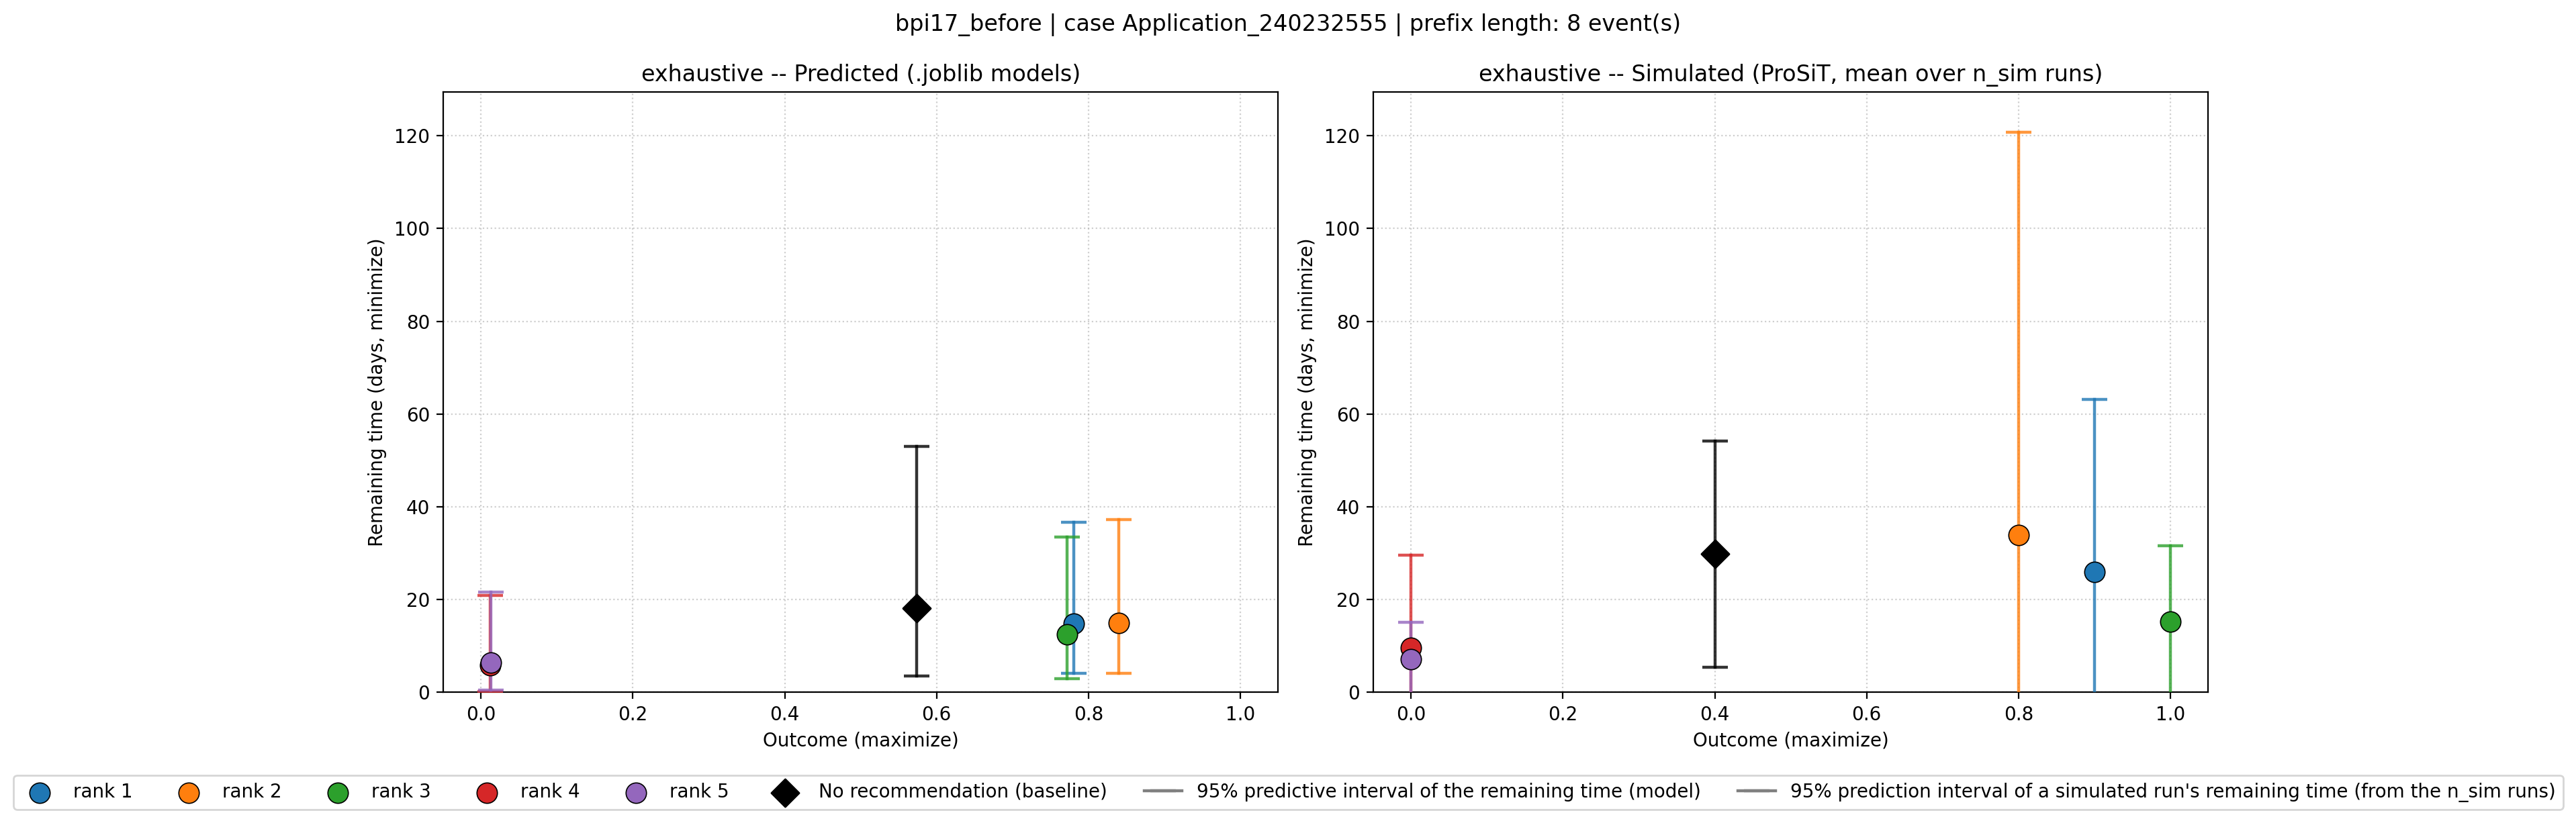
\includegraphics[width=\linewidth]{multi_obj/pareto_fronts/pareto_fronts_predicted_vs_simulated/bpi17_before/bpi17_before_Application_240232555_exhaustive_predicted_vs_simulated.png}
    \end{minipage}
    \hfill
    \begin{minipage}{0.45\textwidth}
        \centering
        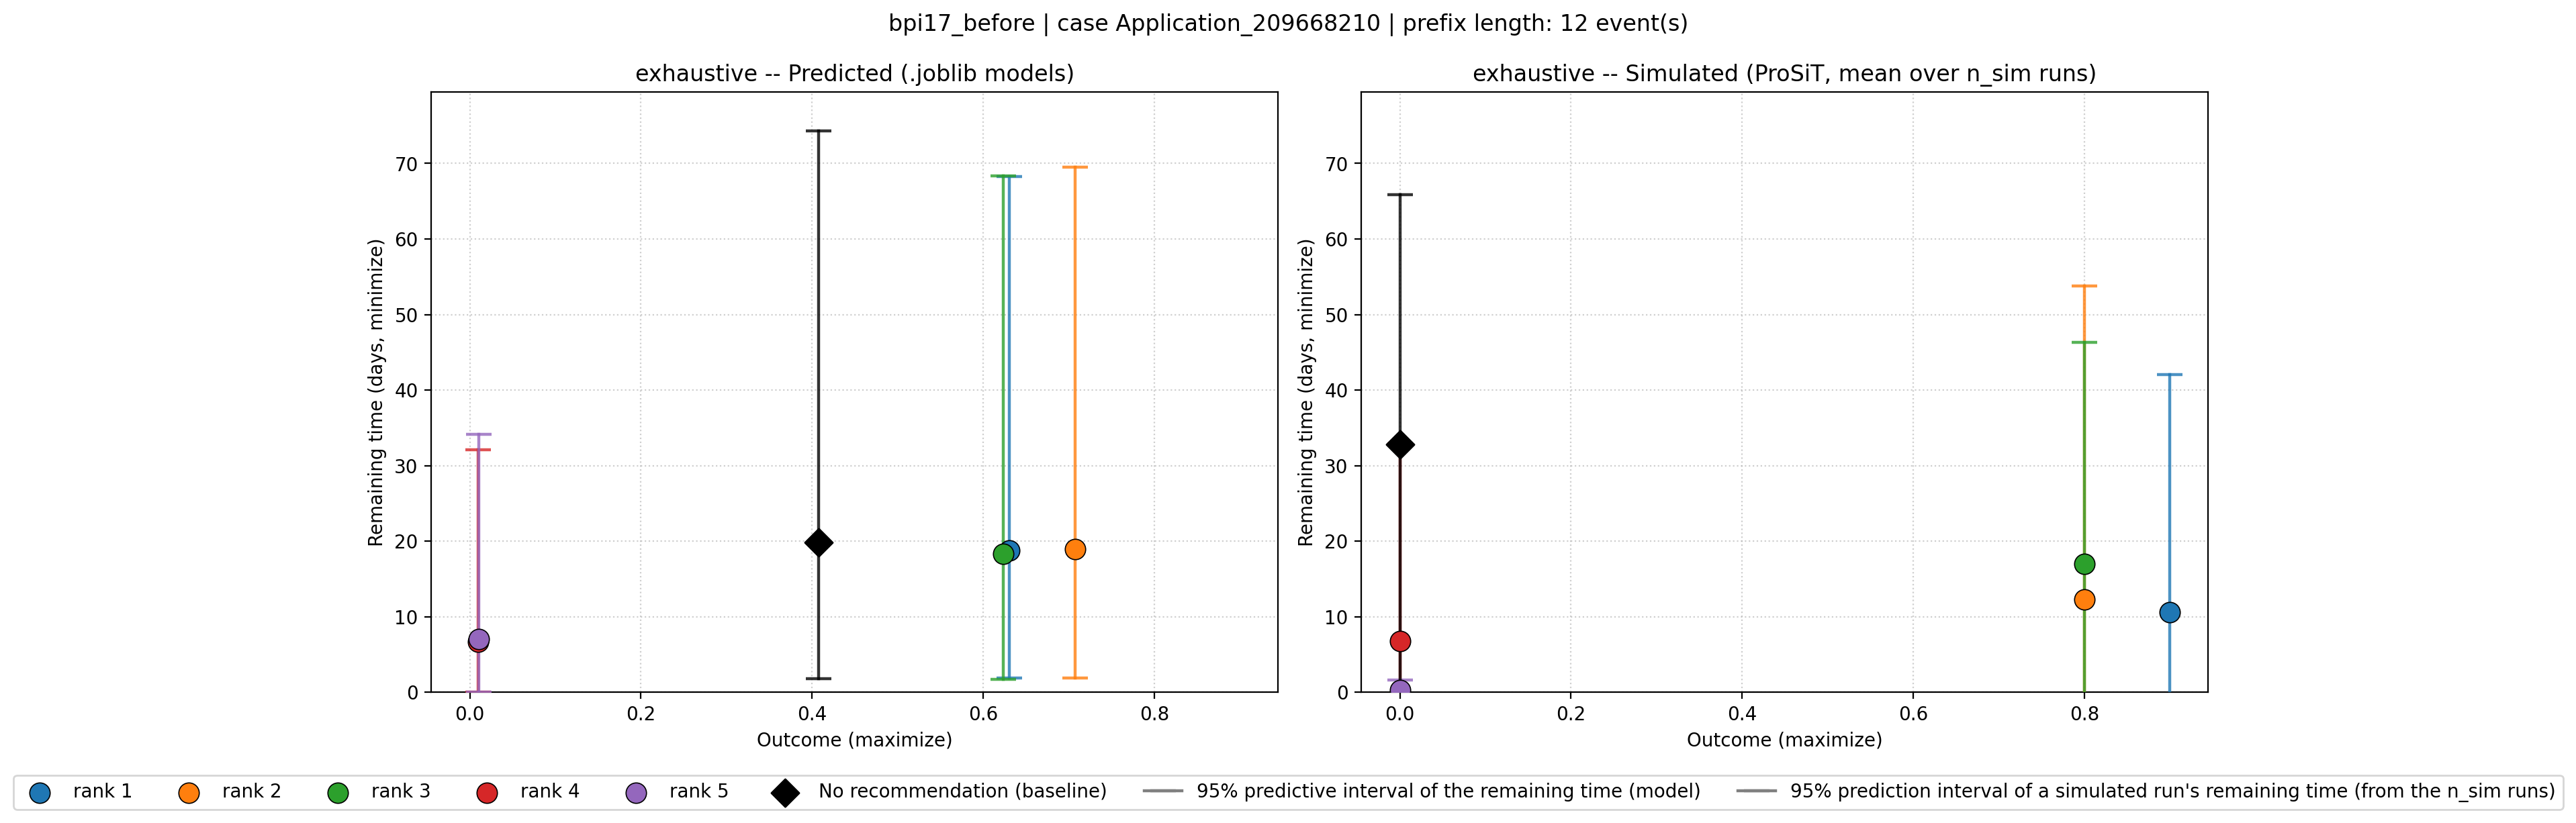
\includegraphics[width=\linewidth]{multi_obj/pareto_fronts/pareto_fronts_predicted_vs_simulated/bpi17_before/bpi17_before_Application_209668210_exhaustive_predicted_vs_simulated.png}
    \end{minipage}
    \vspace{0.4cm}
    \begin{minipage}{0.45\textwidth}
        \centering
        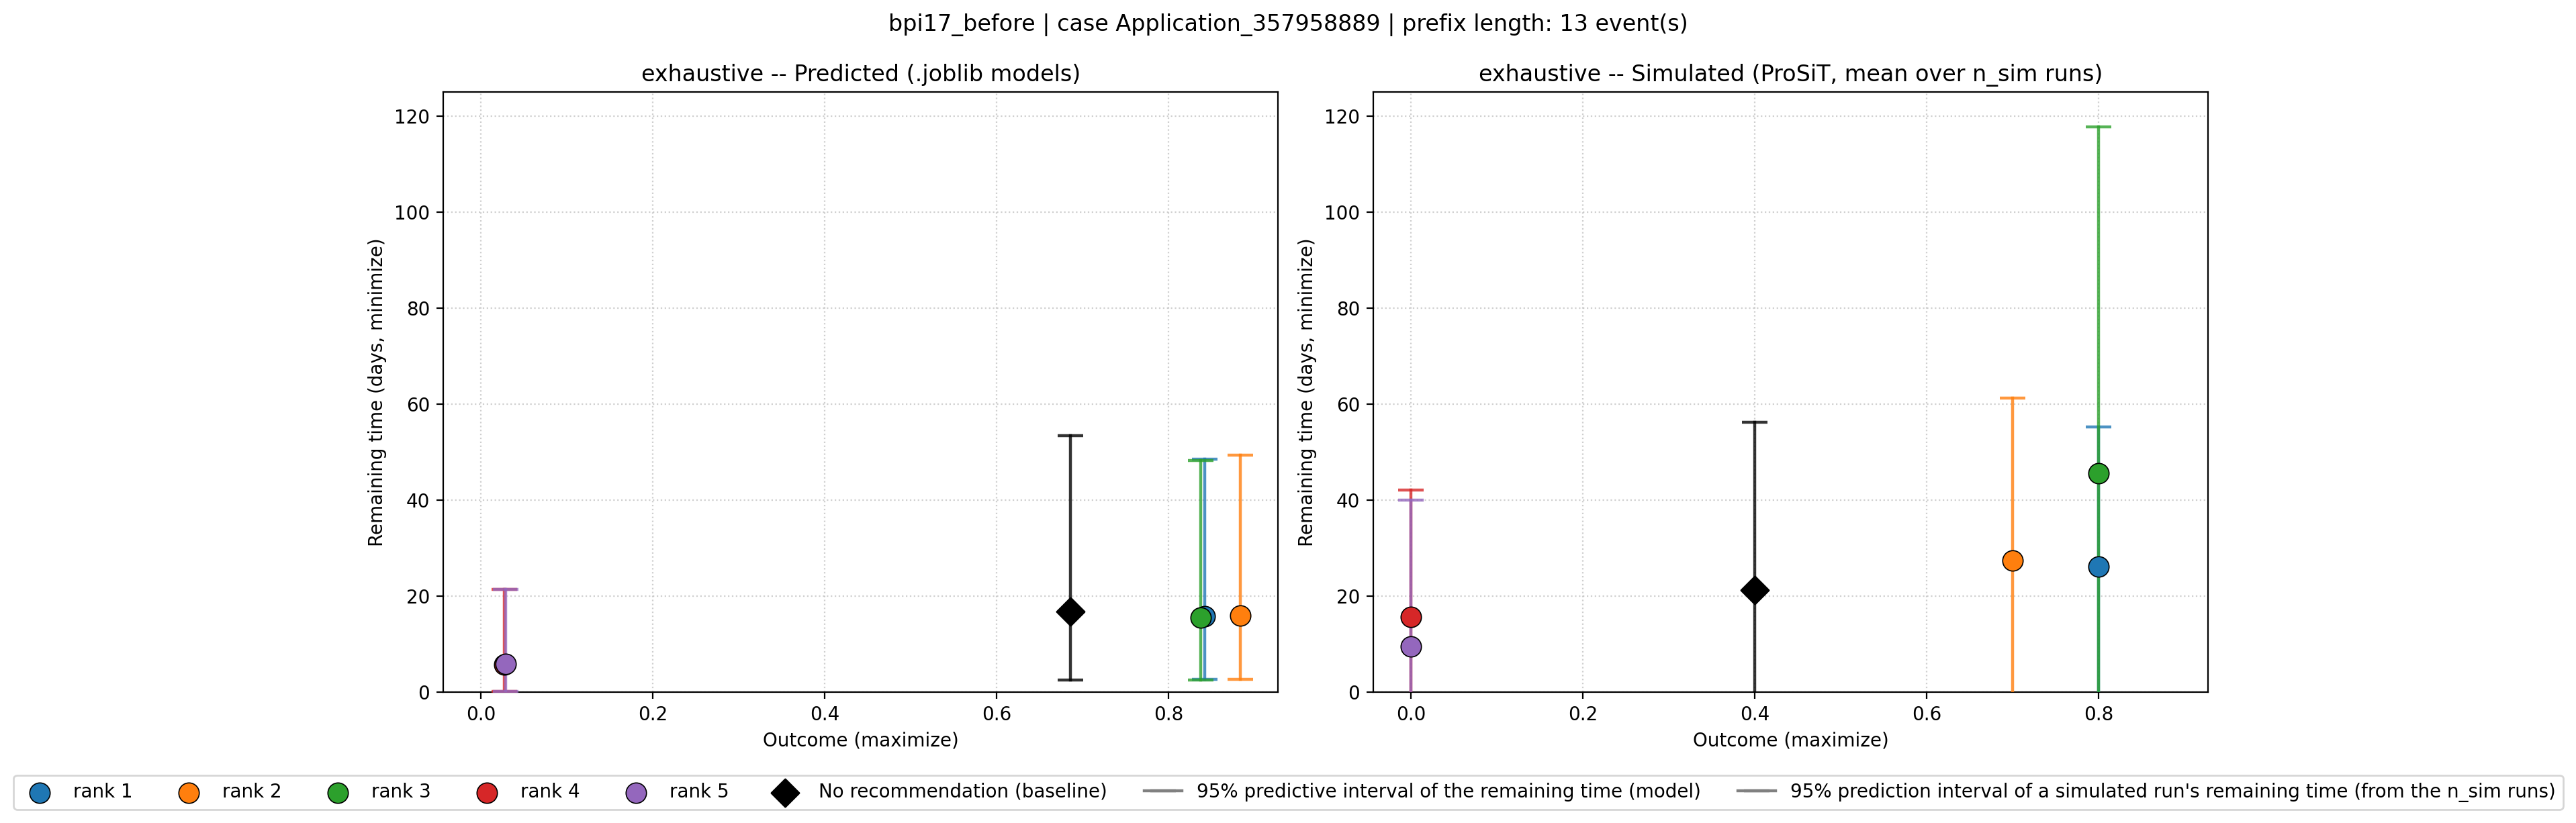
\includegraphics[width=\linewidth]{multi_obj/pareto_fronts/pareto_fronts_predicted_vs_simulated/bpi17_before/bpi17_before_Application_357958889_exhaustive_predicted_vs_simulated.png}
    \end{minipage}
\end{frame}

\begin{frame}{Experimental Results: Predicted vs.\ Simulated (bpi17 after)}
    \centering
    \begin{minipage}{0.45\textwidth}
        \centering
        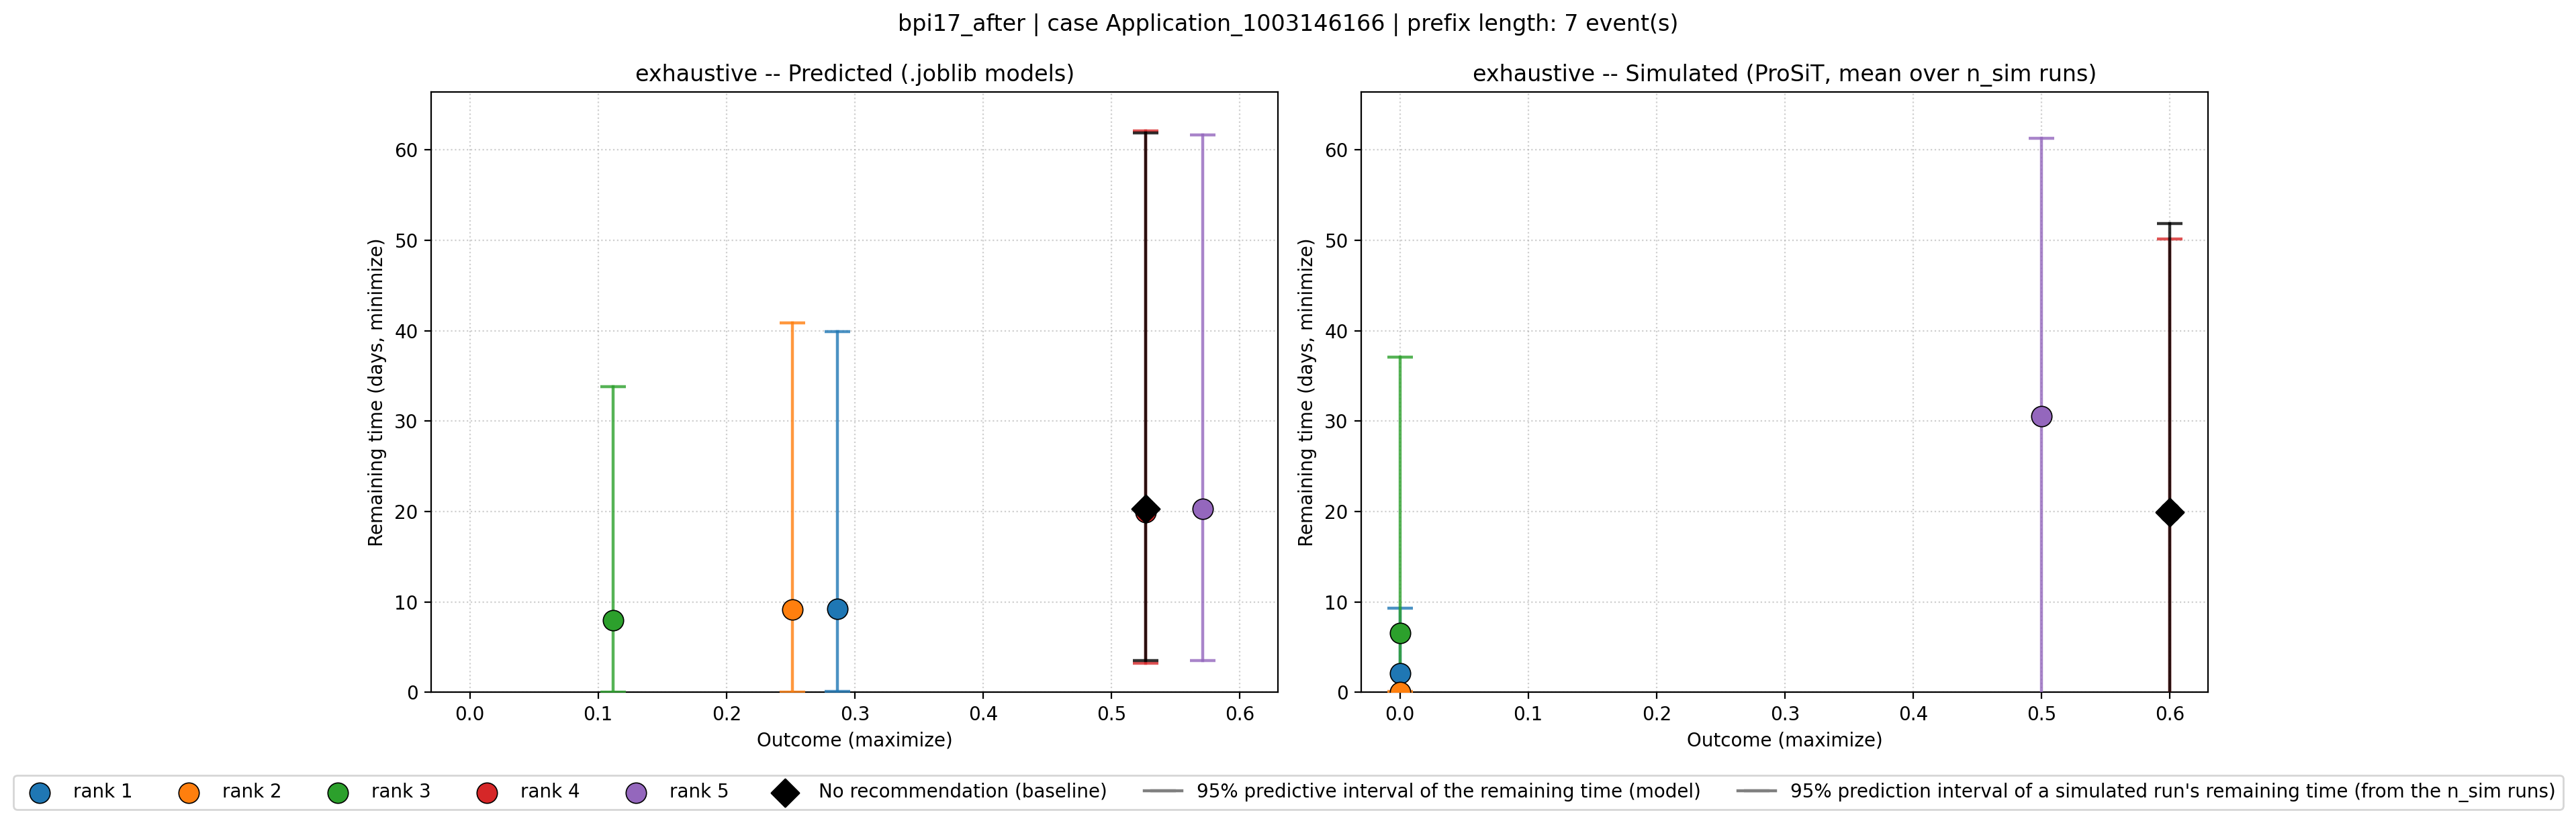
\includegraphics[width=\linewidth]{multi_obj/pareto_fronts/pareto_fronts_predicted_vs_simulated/bpi17_after/bpi17_after_Application_1003146166_exhaustive_predicted_vs_simulated.png}
    \end{minipage}
    \hfill
    \begin{minipage}{0.45\textwidth}
        \centering
        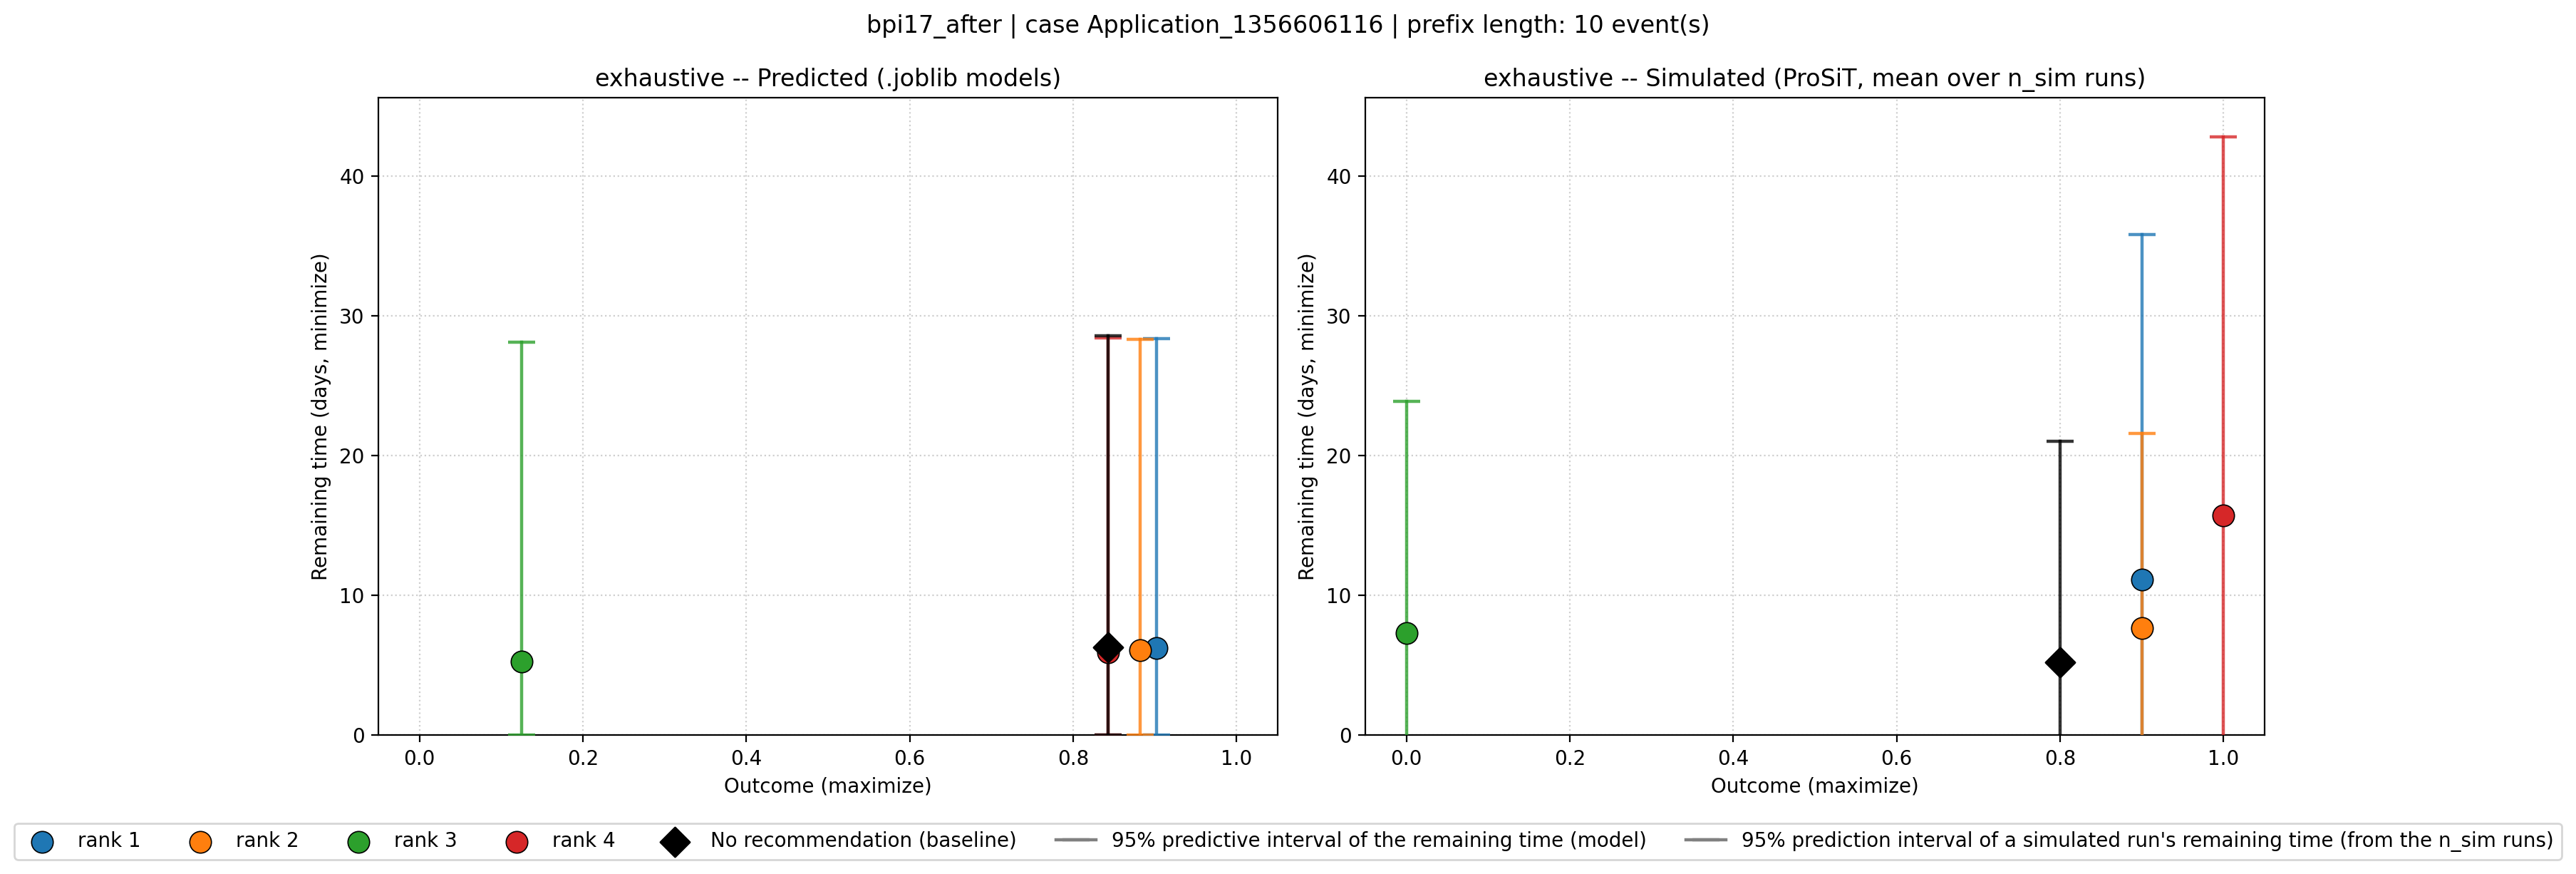
\includegraphics[width=\linewidth]{multi_obj/pareto_fronts/pareto_fronts_predicted_vs_simulated/bpi17_after/bpi17_after_Application_1356606116_exhaustive_predicted_vs_simulated.png}
    \end{minipage}
    \vspace{0.4cm}
    \begin{minipage}{0.45\textwidth}
        \centering
        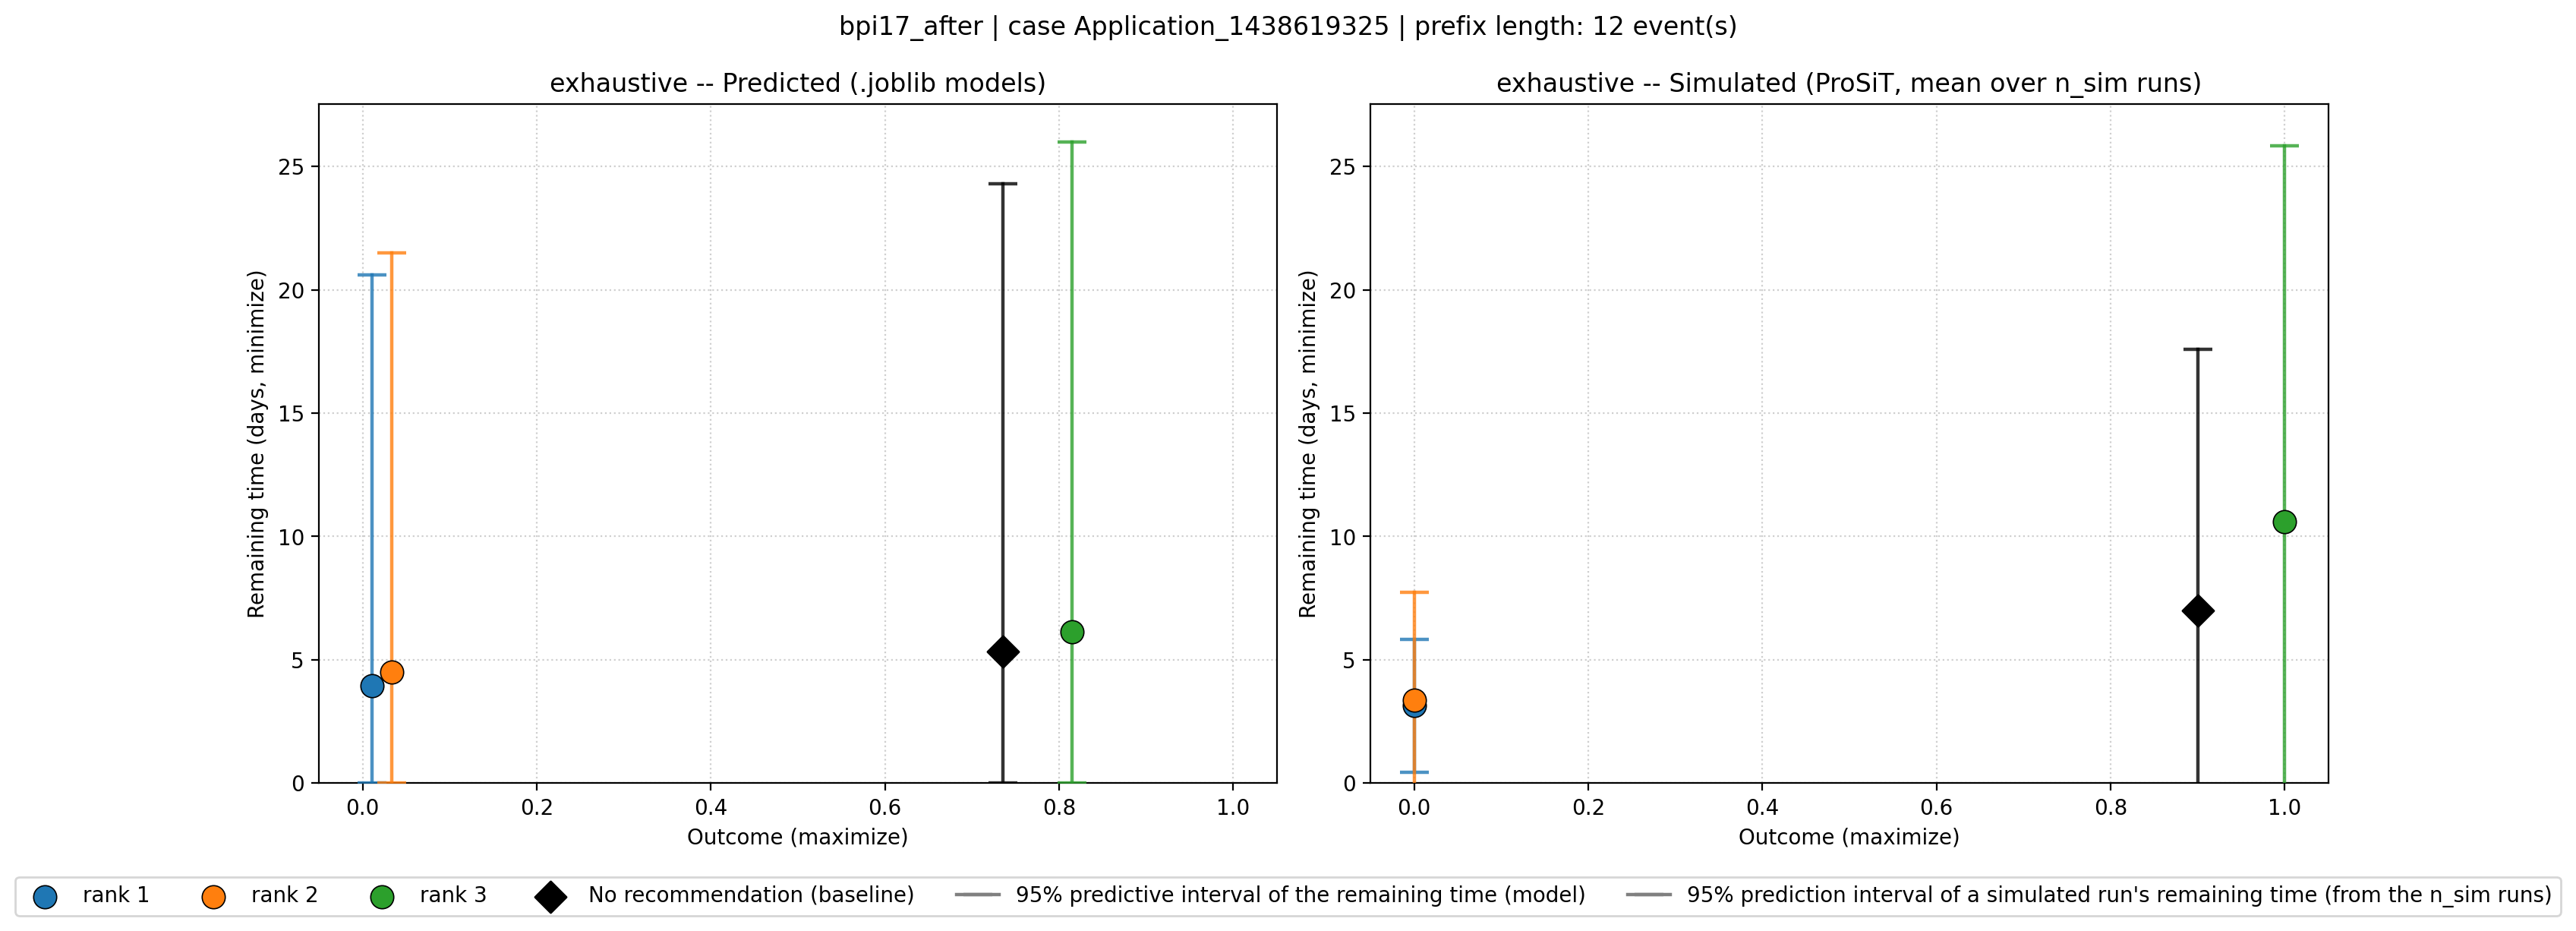
\includegraphics[width=\linewidth]{multi_obj/pareto_fronts/pareto_fronts_predicted_vs_simulated/bpi17_after/bpi17_after_Application_1438619325_exhaustive_predicted_vs_simulated.png}
    \end{minipage}
\end{frame}

% =====================================================================
% Predicted vs simulated over ALL the recommended points (9_prediction_vs_simulation_agreement.py)
% =====================================================================
\begin{frame}{Estimated vs.\ Simulated over All Points: Metrics (1/2)}
  \footnotesize
  \begin{itemize}
    \item \textbf{A point} is a pair (prefix, rank): one of the up to $k = 5$ recommendations of a prefix.
      The rank number is only the order of the candidate list, not a preference: all points are treated alike.
    \item \textbf{Change of each KPI} against the ``no recommendation'' baseline, each on its own side:
      \begin{itemize}\footnotesize
        \item \textbf{outcome}: probability with $-$ without the recommendation, in percentage points (pp);
          estimated: calibrated probability; simulated: share of positive runs over the 10 runs;
        \item \textbf{remaining time}: relative change, \% of the baseline remaining time; estimated: truncated
          log-normal mean; simulated: mean over the 10 runs.
      \end{itemize}
    \item \textbf{Improves}: outcome higher, time shorter. Exception: a simulated outcome positive in all runs both
      with and without the recommendation counts as improved (it cannot do better).
    \item For each KPI a $2\times2$ table: \emph{estimated improves} yes/no $\times$ \emph{simulated improves} yes/no;
      the same for \emph{both KPIs} and for \emph{at least one KPI} (outcome $+$ time $-$ both).
  \end{itemize}
\end{frame}

\begin{frame}{Estimated vs.\ Simulated over All Points: Metrics (2/2)}
  \footnotesize
  \begin{itemize}
    \item \textbf{Good point} ($x = 5$, $y = 10$): improves one KPI by at least $x$ (pp for the outcome, \% for the
      time) and worsens the other by at most $y$; the same rule is applied to the estimated and to the simulated
      changes.
    \item \textbf{Expected value with the recommendation}: $\mathbb{E}_p\big\{\mathbb{E}_r\big[v(p,r)\big]\big\}$,
      the mean of a per-point quantity $v(p,r)$ over the points of a selection: first over the ranks of each
      prefix, then over the prefixes.
    \item Four quantities $v(p,r)$: \textbf{outcome}, \textbf{remaining time}, \textbf{time reduction} and
      \textbf{time won}, each computed twice: from the simulation runs (\emph{simulated}) and from the predictive
      models (\emph{estimated}).
    \item Five selections of points: those that the models estimate to improve \textbf{the outcome}, \textbf{the
      time}, \textbf{both KPIs}, \textbf{at least one KPI}, and the \textbf{good points}.
    \item Formula, selections and quantities in detail: next two slides.
  \end{itemize}
  {\scriptsize Script: \texttt{9\_prediction\_vs\_simulation\_agreement.py} (single runs saved by \texttt{5\_result\_computation.py}).}
\end{frame}

\begin{frame}{Expected Value with the Recommendation: the Formula}
  \scriptsize\setlength{\abovedisplayskip}{2pt}\setlength{\belowdisplayskip}{2pt}
  A \textbf{point} $(p, r)$ is the recommendation $C$ at rank $r$ of prefix $p$. For a selection $\mathcal{S}$ of
  points and a per-point quantity $v(p,r)$:
  \[
    \mathbb{E}_p\Big\{\mathbb{E}_r\big[v(p,r)\big]\Big\}
    \;=\; \frac{1}{|P_{\mathcal{S}}|} \sum_{p \in P_{\mathcal{S}}} \;
    \frac{1}{|R_p|} \sum_{r \in R_p} v(p,r)
  \]
  \vspace{-0.2cm}
  \begin{enumerate}
    \item \textbf{Point}: $v(p,r)$, from the simulation runs or from the predictive models (next slide).
    \item \textbf{Ranks} ($\mathbb{E}_r$): mean over $R_p$, the points of prefix $p$ that are in $\mathcal{S}$ ($|R_p| \le 5$).
    \item \textbf{Prefixes} ($\mathbb{E}_p$): mean over $P_{\mathcal{S}}$, the prefixes with at least one point in
      $\mathcal{S}$. Every prefix weighs the same, whatever its number of points.
  \end{enumerate}
  \textbf{Selections} $\mathcal{S}$, made on the estimated changes only (all that is known when recommending), as if
  only those points were recommended: the points estimated to improve the outcome; to improve the time; to improve
  both KPIs; to improve at least one KPI; the good points. A prefix with no point in $\mathcal{S}$ drops out.

  \textbf{Example} (outcome, simulated, 2 prefixes, 3 points):
  \begin{center}\setlength{\tabcolsep}{5pt}\setlength{\aboverulesep}{0pt}\setlength{\belowrulesep}{1pt}
  \begin{tabular}{ccccc}
    \toprule
    Prefix & Rank & Positive runs & $v(p,r)$ & $\mathbb{E}_r$ \\
    \midrule
    A & 1 & 7 of 10 & 0.7 & $(0.7 + 0.5)/2 = 0.6$ \\
    A & 2 & 5 of 10 & 0.5 & \\
    B & 1 & 9 of 10 & 0.9 & $0.9$ \\
    \bottomrule
  \end{tabular}
  \end{center}
  \vspace{-0.1cm}
  $\mathbb{E}_p = (0.6 + 0.9)/2 = \mathbf{0.75}$ (the plain mean of the 3 points, $0.70$, would count prefix A twice).
\end{frame}

\begin{frame}{Expected Value with the Recommendation: the Four Quantities}
  \scriptsize\setlength{\aboverulesep}{0pt}\setlength{\belowrulesep}{1pt}
  Point $(p, r)$: recommendation $C$; $B$ = no recommendation. \textbf{Simulated}: runs $i = 1, \dots, n_C$ with $C$
  applied ($n_C \le 10$) and $j = 1, \dots, n_B$ without it ($n_B = 10$); $Y^C_i = 1$ if run $i$ ends positive;
  $T^C_i$, $T^B_j$ remaining times (days). \textbf{Estimated}: the predictive models on the encoded prefix with $C$
  ($x_C$) and without it ($x_B$).
  \begin{center}\setlength{\tabcolsep}{4pt}\renewcommand{\arraystretch}{1.15}
  \begin{tabular}{p{1.9cm} p{4.6cm} p{4.6cm}}
    \toprule
    $v(p,r)$ & Simulated & Estimated \\
    \midrule
    Outcome
      & $\frac{1}{n_C}\sum_i Y^C_i$: share of positive runs with $C$
      & $\hat{y}(x_C)$: calibrated probability of a positive outcome with $C$ \\
    Remaining time
      & $\frac{1}{n_C}\sum_i T^C_i$: mean remaining time of the runs with $C$
      & $\hat{T}(x_C)$: estimated remaining time with $C$ (truncated log-normal mean) \\
    Time reduction
      & $\frac{1}{n_B}\sum_j T^B_j - \frac{1}{n_C}\sum_i T^C_i$: mean without $C$ $-$ mean with $C$
      & $\hat{T}(x_B) - \hat{T}(x_C)$: estimated without $C$ $-$ estimated with $C$ \\
    Time won
      & $\frac{1}{n_C n_B}\sum_i\sum_j w_{ij}$, $w_{ij} = 1$ if $T^C_i < T^B_j$, $\tfrac12$ if equal, else $0$: share of the
        (run with $C$, run without) pairs won by $C$
      & $P\big(T(x_C) < T(x_B)\big)$: probability that the time with $C$ is shorter, from the confidence filter \\
    \bottomrule
  \end{tabular}
  \end{center}
  \textbf{Reading}: outcome and remaining time, what to expect following $C$; time reduction, days saved compared with
  no recommendation (positive = shorter); time won, how often $C$ finishes first ($0.5$ = no effect).
\end{frame}

% 2x2 table of 9_prediction_vs_simulation_agreement.txt (sections 1-3): #1 title, #2 est. yes & sim. yes,
% #3 est. yes & sim. no, #4 est. no & sim. yes, #5 est. no & sim. no
\newcommand{\agreementtable}[5]{%
  \begin{minipage}[t]{0.32\textwidth}\vspace{0pt}\centering
    \textbf{#1}\par\vspace{1pt}
    \setlength{\aboverulesep}{0pt}\setlength{\belowrulesep}{1pt}\setlength{\tabcolsep}{4pt}
    \begin{tabular}{lrr}
      \toprule
       & sim.\ yes & sim.\ no \\
      \midrule
      est.\ yes & #2 & #3 \\
      est.\ no  & #4 & #5 \\
      \bottomrule
    \end{tabular}
  \end{minipage}}

% === BEGIN 9 agreement slides (generated from 9_prediction_vs_simulation_agreement.csv: rerun 9_slides_from_csv_v2.py or edit the numbers by hand) ===

\begin{frame}{Estimated vs.\ Simulated (BAC): the Five Tables}
  \footnotesize
  2293 recommended points in 1871 prefixes. Rows: the models estimate an improvement; columns: the
  simulation shows it (mean over the 10 runs).
  \par\vspace{0.3cm}\noindent
  \agreementtable{Outcome}{1013}{865}{212}{203}\hfill
  \agreementtable{Remaining time}{985}{723}{267}{318}\hfill
  \agreementtable{At least one KPI}{1718}{566}{3}{6}
  \par\vspace{0.5cm}\noindent\hspace*{\fill}%
  \agreementtable{Both KPIs}{457}{845}{299}{692}\hspace{0.08\textwidth}%
  \agreementtable{Good points ($x = 5$, $y = 10$)}{355}{153}{870}{915}\hspace*{\fill}
\end{frame}

\begin{frame}{Estimated vs.\ Simulated (BAC): Summary}
  \footnotesize\setlength{\aboverulesep}{0pt}\setlength{\belowrulesep}{1pt}
  2293 recommended points in 1871 prefixes.
  \begin{center}\setlength{\tabcolsep}{6pt}
  \begin{tabular}{lcc}
    \toprule
     & estimated improves & estimated and simulated improve \\
    \midrule
    Outcome & 1878 (81.9\%) & 1013 (44.2\%) \\
    Remaining time & 1708 (74.5\%) & 985 (43.0\%) \\
    At least one KPI & 2284 (99.6\%) & 1718 (74.9\%) \\
    Both KPIs & 1302 (56.8\%) & 457 (19.9\%) \\
    Good points & 508 (22.2\%) & 355 (15.5\%) \\
    \bottomrule
  \end{tabular}
  \end{center}
  {\scriptsize Number of points and, in brackets, their share of all the 2293 recommended points.}
\end{frame}

\begin{frame}{Estimated vs.\ Simulated (BAC): Expected Values}
  \scriptsize\setlength{\aboverulesep}{0pt}\setlength{\belowrulesep}{1pt}
  \textbf{Expected value with the recommendation}, $\mathbb{E}_p\big\{\mathbb{E}_r\big[v(p,r)\big]\big\}$,
  on the points of each table that the models estimate to improve (columns 1--4) or to be good (column 5).
  \begin{center}\setlength{\tabcolsep}{3pt}
  \begin{tabular}{ll ccccc}
    \toprule
     & & \multicolumn{4}{c}{Estimated to improve} & \\
    \cmidrule(lr){3-6}
     & & outcome & time & both & at least one & Good points \\
    \midrule
    Points & & 1878 & 1708 & 1302 & 2284 & 508 \\
    Prefixes covered & & 1745 (93\%) & 1532 (82\%) & 1273 (68\%) & 1870 (100\%) & 460 (25\%) \\
    \midrule
    Outcome (share / prob.) & simulated & 0.833 & 0.820 & 0.837 & 0.813 & 0.797 \\
     & estimated & 0.833 & 0.801 & 0.829 & 0.803 & 0.801 \\
    \addlinespace[2pt]
    Remaining time (days) & simulated & 9.02 & 6.69 & 6.63 & 8.63 & 7.56 \\
     & estimated & 8.20 & 6.75 & 6.23 & 8.15 & 8.74 \\
    \addlinespace[2pt]
    Time reduction (days) & simulated & $-0.08$ & $+1.15$ & $+0.53$ & $+0.35$ & $+4.63$ \\
     & estimated & $+0.24$ & $+0.74$ & $+0.51$ & $+0.38$ & $+2.50$ \\
    \addlinespace[2pt]
    Time won (share / prob.) & simulated & 0.506 & 0.526 & 0.519 & 0.513 & 0.582 \\
     & estimated & 0.512 & 0.521 & 0.519 & 0.514 & 0.567 \\
    \bottomrule
  \end{tabular}
  \end{center}
  {\tiny Time reduction: baseline $-$ with the recommendation (positive = shorter). Time won: $0.5$ = no effect.
  Prefixes covered: prefixes with at least one point of the column, of 1871. Definitions: ``the Four Quantities''.}
\end{frame}

\begin{frame}{Estimated vs.\ Simulated (BPI12): the Five Tables}
  \footnotesize
  978 recommended points in 601 prefixes. Rows: the models estimate an improvement; columns: the
  simulation shows it (mean over the 10 runs).
  \par\vspace{0.3cm}\noindent
  \agreementtable{Outcome}{490}{115}{1}{372}\hfill
  \agreementtable{Remaining time}{635}{198}{27}{118}\hfill
  \agreementtable{At least one KPI}{831}{116}{13}{18}
  \par\vspace{0.5cm}\noindent\hspace*{\fill}%
  \agreementtable{Both KPIs}{296}{195}{13}{474}\hspace{0.08\textwidth}%
  \agreementtable{Good points ($x = 5$, $y = 10$)}{377}{124}{20}{457}\hspace*{\fill}
\end{frame}

\begin{frame}{Estimated vs.\ Simulated (BPI12): Summary}
  \footnotesize\setlength{\aboverulesep}{0pt}\setlength{\belowrulesep}{1pt}
  978 recommended points in 601 prefixes.
  \begin{center}\setlength{\tabcolsep}{6pt}
  \begin{tabular}{lcc}
    \toprule
     & estimated improves & estimated and simulated improve \\
    \midrule
    Outcome & 605 (61.9\%) & 490 (50.1\%) \\
    Remaining time & 833 (85.2\%) & 635 (64.9\%) \\
    At least one KPI & 947 (96.8\%) & 831 (85.0\%) \\
    Both KPIs & 491 (50.2\%) & 296 (30.3\%) \\
    Good points & 501 (51.2\%) & 377 (38.5\%) \\
    \bottomrule
  \end{tabular}
  \end{center}
  {\scriptsize Number of points and, in brackets, their share of all the 978 recommended points.}
\end{frame}

\begin{frame}{Estimated vs.\ Simulated (BPI12): Expected Values}
  \scriptsize\setlength{\aboverulesep}{0pt}\setlength{\belowrulesep}{1pt}
  \textbf{Expected value with the recommendation}, $\mathbb{E}_p\big\{\mathbb{E}_r\big[v(p,r)\big]\big\}$,
  on the points of each table that the models estimate to improve (columns 1--4) or to be good (column 5).
  \begin{center}\setlength{\tabcolsep}{3pt}
  \begin{tabular}{ll ccccc}
    \toprule
     & & \multicolumn{4}{c}{Estimated to improve} & \\
    \cmidrule(lr){3-6}
     & & outcome & time & both & at least one & Good points \\
    \midrule
    Points & & 605 & 833 & 491 & 947 & 501 \\
    Prefixes covered & & 600 (100\%) & 590 (98\%) & 488 (81\%) & 601 (100\%) & 498 (83\%) \\
    \midrule
    Outcome (share / prob.) & simulated & 0.749 & 0.509 & 0.720 & 0.582 & 0.724 \\
     & estimated & 0.721 & 0.514 & 0.697 & 0.577 & 0.701 \\
    \addlinespace[2pt]
    Remaining time (days) & simulated & 14.27 & 12.53 & 15.27 & 12.83 & 15.12 \\
     & estimated & 14.45 & 14.13 & 16.20 & 14.11 & 15.97 \\
    \addlinespace[2pt]
    Time reduction (days) & simulated & $+1.43$ & $+3.35$ & $+2.82$ & $+2.87$ & $+2.74$ \\
     & estimated & $+0.82$ & $+1.36$ & $+1.38$ & $+1.17$ & $+1.35$ \\
    \addlinespace[2pt]
    Time won (share / prob.) & simulated & 0.503 & 0.577 & 0.559 & 0.556 & 0.556 \\
     & estimated & 0.505 & 0.528 & 0.522 & 0.521 & 0.522 \\
    \bottomrule
  \end{tabular}
  \end{center}
  {\tiny Time reduction: baseline $-$ with the recommendation (positive = shorter). Time won: $0.5$ = no effect.
  Prefixes covered: prefixes with at least one point of the column, of 601. Definitions: ``the Four Quantities''.}
\end{frame}

\begin{frame}{Estimated vs.\ Simulated (bpi17-before): the Five Tables}
  \footnotesize
  1436 recommended points in 1168 prefixes. Rows: the models estimate an improvement; columns: the
  simulation shows it (mean over the 10 runs).
  \par\vspace{0.3cm}\noindent
  \agreementtable{Outcome}{1007}{290}{17}{122}\hfill
  \agreementtable{Remaining time}{1055}{315}{28}{38}\hfill
  \agreementtable{At least one KPI}{1291}{145}{0}{0}
  \par\vspace{0.5cm}\noindent\hspace*{\fill}%
  \agreementtable{Both KPIs}{783}{448}{33}{172}\hspace{0.08\textwidth}%
  \agreementtable{Good points ($x = 5$, $y = 10$)}{933}{238}{81}{184}\hspace*{\fill}
\end{frame}

\begin{frame}{Estimated vs.\ Simulated (bpi17-before): Summary}
  \footnotesize\setlength{\aboverulesep}{0pt}\setlength{\belowrulesep}{1pt}
  1436 recommended points in 1168 prefixes.
  \begin{center}\setlength{\tabcolsep}{6pt}
  \begin{tabular}{lcc}
    \toprule
     & estimated improves & estimated and simulated improve \\
    \midrule
    Outcome & 1297 (90.3\%) & 1007 (70.1\%) \\
    Remaining time & 1370 (95.4\%) & 1055 (73.5\%) \\
    At least one KPI & 1436 (100.0\%) & 1291 (89.9\%) \\
    Both KPIs & 1231 (85.7\%) & 783 (54.5\%) \\
    Good points & 1171 (81.5\%) & 933 (65.0\%) \\
    \bottomrule
  \end{tabular}
  \end{center}
  {\scriptsize Number of points and, in brackets, their share of all the 1436 recommended points.}
\end{frame}

\begin{frame}{Estimated vs.\ Simulated (bpi17-before): Expected Values}
  \scriptsize\setlength{\aboverulesep}{0pt}\setlength{\belowrulesep}{1pt}
  \textbf{Expected value with the recommendation}, $\mathbb{E}_p\big\{\mathbb{E}_r\big[v(p,r)\big]\big\}$,
  on the points of each table that the models estimate to improve (columns 1--4) or to be good (column 5).
  \begin{center}\setlength{\tabcolsep}{3pt}
  \begin{tabular}{ll ccccc}
    \toprule
     & & \multicolumn{4}{c}{Estimated to improve} & \\
    \cmidrule(lr){3-6}
     & & outcome & time & both & at least one & Good points \\
    \midrule
    Points & & 1297 & 1370 & 1231 & 1436 & 1171 \\
    Prefixes covered & & 1136 (97\%) & 1163 (100\%) & 1096 (94\%) & 1168 (100\%) & 1058 (91\%) \\
    \midrule
    Outcome (share / prob.) & simulated & 0.800 & 0.746 & 0.795 & 0.761 & 0.795 \\
     & estimated & 0.789 & 0.738 & 0.785 & 0.751 & 0.782 \\
    \addlinespace[2pt]
    Remaining time (days) & simulated & 13.25 & 13.39 & 13.47 & 13.43 & 13.70 \\
     & estimated & 14.43 & 14.36 & 14.73 & 14.37 & 15.00 \\
    \addlinespace[2pt]
    Time reduction (days) & simulated & $+3.92$ & $+3.90$ & $+4.12$ & $+3.84$ & $+4.21$ \\
     & estimated & $+2.79$ & $+3.02$ & $+2.94$ & $+2.95$ & $+3.04$ \\
    \addlinespace[2pt]
    Time won (share / prob.) & simulated & 0.582 & 0.589 & 0.590 & 0.584 & 0.593 \\
     & estimated & 0.546 & 0.557 & 0.551 & 0.554 & 0.553 \\
    \bottomrule
  \end{tabular}
  \end{center}
  {\tiny Time reduction: baseline $-$ with the recommendation (positive = shorter). Time won: $0.5$ = no effect.
  Prefixes covered: prefixes with at least one point of the column, of 1168. Definitions: ``the Four Quantities''.}
\end{frame}

\begin{frame}{Estimated vs.\ Simulated (bpi17-after): the Five Tables}
  \footnotesize
  2345 recommended points in 1799 prefixes. Rows: the models estimate an improvement; columns: the
  simulation shows it (mean over the 10 runs).
  \par\vspace{0.3cm}\noindent
  \agreementtable{Outcome}{1240}{558}{5}{542}\hfill
  \agreementtable{Remaining time}{1533}{666}{60}{86}\hfill
  \agreementtable{At least one KPI}{1876}{465}{2}{2}
  \par\vspace{0.5cm}\noindent\hspace*{\fill}%
  \agreementtable{Both KPIs}{934}{722}{26}{663}\hspace{0.08\textwidth}%
  \agreementtable{Good points ($x = 5$, $y = 10$)}{1095}{279}{148}{823}\hspace*{\fill}
\end{frame}

\begin{frame}{Estimated vs.\ Simulated (bpi17-after): Summary}
  \footnotesize\setlength{\aboverulesep}{0pt}\setlength{\belowrulesep}{1pt}
  2345 recommended points in 1799 prefixes.
  \begin{center}\setlength{\tabcolsep}{6pt}
  \begin{tabular}{lcc}
    \toprule
     & estimated improves & estimated and simulated improve \\
    \midrule
    Outcome & 1798 (76.7\%) & 1240 (52.9\%) \\
    Remaining time & 2199 (93.8\%) & 1533 (65.4\%) \\
    At least one KPI & 2341 (99.8\%) & 1876 (80.0\%) \\
    Both KPIs & 1656 (70.6\%) & 934 (39.8\%) \\
    Good points & 1374 (58.6\%) & 1095 (46.7\%) \\
    \bottomrule
  \end{tabular}
  \end{center}
  {\scriptsize Number of points and, in brackets, their share of all the 2345 recommended points.}
\end{frame}

\begin{frame}{Estimated vs.\ Simulated (bpi17-after): Expected Values}
  \scriptsize\setlength{\aboverulesep}{0pt}\setlength{\belowrulesep}{1pt}
  \textbf{Expected value with the recommendation}, $\mathbb{E}_p\big\{\mathbb{E}_r\big[v(p,r)\big]\big\}$,
  on the points of each table that the models estimate to improve (columns 1--4) or to be good (column 5).
  \begin{center}\setlength{\tabcolsep}{3pt}
  \begin{tabular}{ll ccccc}
    \toprule
     & & \multicolumn{4}{c}{Estimated to improve} & \\
    \cmidrule(lr){3-6}
     & & outcome & time & both & at least one & Good points \\
    \midrule
    Points & & 1798 & 2199 & 1656 & 2341 & 1374 \\
    Prefixes covered & & 1784 (99\%) & 1751 (97\%) & 1656 (92\%) & 1796 (100\%) & 1374 (76\%) \\
    \midrule
    Outcome (share / prob.) & simulated & 0.788 & 0.652 & 0.786 & 0.676 & 0.780 \\
     & estimated & 0.767 & 0.638 & 0.760 & 0.663 & 0.739 \\
    \addlinespace[2pt]
    Remaining time (days) & simulated & 14.37 & 14.33 & 14.76 & 14.34 & 16.16 \\
     & estimated & 15.31 & 15.31 & 15.95 & 15.14 & 18.05 \\
    \addlinespace[2pt]
    Time reduction (days) & simulated & $+3.03$ & $+3.24$ & $+3.32$ & $+3.06$ & $+4.08$ \\
     & estimated & $+0.69$ & $+0.94$ & $+0.77$ & $+0.88$ & $+0.91$ \\
    \addlinespace[2pt]
    Time won (share / prob.) & simulated & 0.573 & 0.586 & 0.583 & 0.579 & 0.606 \\
     & estimated & 0.505 & 0.516 & 0.507 & 0.514 & 0.508 \\
    \bottomrule
  \end{tabular}
  \end{center}
  {\tiny Time reduction: baseline $-$ with the recommendation (positive = shorter). Time won: $0.5$ = no effect.
  Prefixes covered: prefixes with at least one point of the column, of 1799. Definitions: ``the Four Quantities''.}
\end{frame}

\begin{frame}{Estimated vs.\ Simulated (\texttt{BPI12\_sim}): the Five Tables}
  \footnotesize
  924 recommended points in 623 prefixes. Rows: the models estimate an improvement; columns: the
  simulation shows it (mean over the 10 runs).
  \par\vspace{0.3cm}\noindent
  \agreementtable{Outcome}{619}{162}{11}{132}\hfill
  \agreementtable{Remaining time}{557}{169}{15}{183}\hfill
  \agreementtable{At least one KPI}{802}{108}{5}{9}
  \par\vspace{0.5cm}\noindent\hspace*{\fill}%
  \agreementtable{Both KPIs}{376}{221}{19}{308}\hspace{0.08\textwidth}%
  \agreementtable{Good points ($x = 5$, $y = 10$)}{481}{120}{30}{293}\hspace*{\fill}
\end{frame}

\begin{frame}{Estimated vs.\ Simulated (\texttt{BPI12\_sim}): Summary}
  \footnotesize\setlength{\aboverulesep}{0pt}\setlength{\belowrulesep}{1pt}
  924 recommended points in 623 prefixes.
  \begin{center}\setlength{\tabcolsep}{6pt}
  \begin{tabular}{lcc}
    \toprule
     & estimated improves & estimated and simulated improve \\
    \midrule
    Outcome & 781 (84.5\%) & 619 (67.0\%) \\
    Remaining time & 726 (78.6\%) & 557 (60.3\%) \\
    At least one KPI & 910 (98.5\%) & 802 (86.8\%) \\
    Both KPIs & 597 (64.6\%) & 376 (40.7\%) \\
    Good points & 601 (65.0\%) & 481 (52.1\%) \\
    \bottomrule
  \end{tabular}
  \end{center}
  {\scriptsize Number of points and, in brackets, their share of all the 924 recommended points.}
\end{frame}

\begin{frame}{Estimated vs.\ Simulated (\texttt{BPI12\_sim}): Expected Values}
  \scriptsize\setlength{\aboverulesep}{0pt}\setlength{\belowrulesep}{1pt}
  \textbf{Expected value with the recommendation}, $\mathbb{E}_p\big\{\mathbb{E}_r\big[v(p,r)\big]\big\}$,
  on the points of each table that the models estimate to improve (columns 1--4) or to be good (column 5).
  \begin{center}\setlength{\tabcolsep}{3pt}
  \begin{tabular}{ll ccccc}
    \toprule
     & & \multicolumn{4}{c}{Estimated to improve} & \\
    \cmidrule(lr){3-6}
     & & outcome & time & both & at least one & Good points \\
    \midrule
    Points & & 781 & 726 & 597 & 910 & 601 \\
    Prefixes covered & & 600 (96\%) & 609 (98\%) & 491 (79\%) & 623 (100\%) & 493 (79\%) \\
    \midrule
    Outcome (share / prob.) & simulated & 0.736 & 0.585 & 0.706 & 0.674 & 0.706 \\
     & estimated & 0.741 & 0.599 & 0.721 & 0.682 & 0.722 \\
    \addlinespace[2pt]
    Remaining time (days) & simulated & 14.32 & 13.55 & 15.10 & 14.08 & 15.05 \\
     & estimated & 14.72 & 14.72 & 16.37 & 14.73 & 16.31 \\
    \addlinespace[2pt]
    Time reduction (days) & simulated & $+1.54$ & $+2.68$ & $+3.07$ & $+1.91$ & $+3.06$ \\
     & estimated & $+1.12$ & $+1.51$ & $+1.80$ & $+1.23$ & $+1.79$ \\
    \addlinespace[2pt]
    Time won (share / prob.) & simulated & 0.512 & 0.566 & 0.569 & 0.530 & 0.568 \\
     & estimated & 0.509 & 0.528 & 0.531 & 0.516 & 0.530 \\
    \bottomrule
  \end{tabular}
  \end{center}
  {\tiny Time reduction: baseline $-$ with the recommendation (positive = shorter). Time won: $0.5$ = no effect.
  Prefixes covered: prefixes with at least one point of the column, of 623. Definitions: ``the Four Quantities''.}
\end{frame}
% === END 9 agreement slides ===

% Previous result slides (old "% of comparisons won" metric, recommendations before the resource threshold of
% 2026-10-21): kept out of the build, replaced by the per-dataset slides above.
\iffalse
\begin{frame}{Predicted vs.\ Simulated: Is the Predicted Improvement Confirmed?}
  \footnotesize
  All recommended points; \% of points (pred.), shares in \% and discrimination in pp.
  \begin{center}\scriptsize\setlength{\tabcolsep}{3.5pt}
  \begin{tabular}{l cccc cccc cc}
    \toprule
     & \multicolumn{4}{c}{Outcome} & \multicolumn{4}{c}{Remaining time} & \multicolumn{2}{c}{Both KPIs} \\
    \cmidrule(lr){2-5}\cmidrule(lr){6-9}\cmidrule(lr){10-11}
    Case study & pred. & confirmed & ref. & discr. & pred. & confirmed & ref. & discr. & confirmed & discr. \\
    \midrule
    BAC                 & 93 & 52 & 46 & $+6$  & 78 & 52 & 43 & $+9$  & 33 & $+11$ \\
    BPI12               & 64 & 75 &  6 & $+69$ & 78 & 69 & 17 & $+51$ & 49 & $+46$ \\
    bpi17-before        & 62 & 76 &  2 & $+75$ & 97 & 68 & 39 & $+30$ & 43 & $+41$ \\
    bpi17-after         & 54 & 73 &  2 & $+71$ & 95 & 64 & 33 & $+32$ & 32 & $+30$ \\
    \texttt{BPI12\_sim} & 53 & 76 &  1 & $+75$ & 83 & 74 & 10 & $+64$ & 48 & $+46$ \\
    \bottomrule
  \end{tabular}
  \end{center}
  \scriptsize
  \begin{itemize}
    \item \textbf{Outcome}: if the model says ``no'' the simulation almost never improves (1--6\%), if it says
      ``yes'' it does about 3 times out of 4 (discrimination $+69$ to $+75$); the rest is model error and noise of 10 runs.
    \item \textbf{Time}: weaker ($+30$ to $+64$): the predicted time effects are small compared to the noise.
    \item \textbf{Both KPIs}: about the product of the two single confirmations.
    \item \textbf{BAC} ($+6$ / $+9$): the actions barely change the process (outcome gain $+1.2$ pp), within the noise.
  \end{itemize}
  {\scriptsize Source: \texttt{9\_prediction\_vs\_simulation\_agreement.txt}.}
\end{frame}

\begin{frame}{Predicted vs.\ Simulated: Good Points and Effective Gain}
  \footnotesize
  Good points with $x = 5$, $y = 10$; effective gain as simulated / expected.
  \begin{center}\scriptsize\setlength{\tabcolsep}{2.5pt}
  \begin{tabular}{l ccc cc cc}
    \toprule
     & \multicolumn{3}{c}{Good points} & \multicolumn{2}{c}{Outcome gain (pp)} & \multicolumn{2}{c}{Time: \% won} \\
    \cmidrule(lr){2-4}\cmidrule(lr){5-6}\cmidrule(lr){7-8}
    Case study & \% points & \% prefixes & good in sim. & all points & good only & all points & good only \\
    \midrule
    BAC                 & 26 & 28 & 53 & $+1.2$ / $+1.3$   & $+2.2$ / $+3.7$   & 50.3 / 51.3 & 51.7 / 55.7 \\
    BPI12               & 50 & 85 & 66 & $+7.1$ / $+8.6$   & $+22.0$ / $+23.3$ & 53.3 / 59.7 & 54.9 / 61.3 \\
    bpi17-before        & 60 & 96 & 59 & $-7.9$ / $-7.7$   & $+19.1$ / $+19.0$ & 57.2 / 65.7 & 51.7 / 57.6 \\
    bpi17-after         & 50 & 92 & 48 & $-16.3$ / $-17.0$ & $+18.4$ / $+15.1$ & 56.3 / 55.9 & 47.7 / 50.9 \\
    \texttt{BPI12\_sim} & 35 & 78 & 66 & $-7.4$ / $-1.8$   & $+23.9$ / $+31.2$ & 55.5 / 54.7 & 53.3 / 52.1 \\
    \bottomrule
  \end{tabular}
  \end{center}
  \scriptsize
  \begin{itemize}
    \item \textbf{All points}: on bpi17 the mean outcome gain is negative: the $p$-dispersion spreads the $k$
      points over the whole front, including actions that trade the outcome for the time.
    \item \textbf{Good points only}: $+18$ to $+22$ pp on BPI12 and bpi17, confirmed by the simulator (within 3.3 pp;
      \texttt{BPI12\_sim} $+23.9$ vs.\ $+31.2$); 4--22\% of the prefixes are left without recommendation (72\% on BAC).
    \item \textbf{Time}: the model is optimistic (BPI12: 61.3\% expected, 54.9\% simulated); restricted to the good
      points the time effect is about neutral (\% won = 50\% means no effect).
  \end{itemize}
  {\scriptsize Source: \texttt{9\_prediction\_vs\_simulation\_agreement.txt}.}
\end{frame}

\begin{frame}{bpi17-after: Why the Good Points Do Not Shorten the Time}
  \footnotesize
  Simulated effect by recommended activity (largest groups).
  \begin{center}\scriptsize
  \begin{tabular}{llccc}
    \toprule
    Points & Activity & Points & Time: \% comparisons won & Outcome change (pp) \\
    \midrule
    not good & \texttt{A\_Cancelled}    & 1782 & 68 & $-59.8$ \\
    not good & \texttt{A\_Denied}       &  162 & 72 & $-78.0$ \\
    good     & \texttt{A\_Validating}   & 2134 & 49 & $+20.0$ \\
    good     & \texttt{O\_Create Offer} &   82 & 32 & $-12.2$ \\
    \bottomrule
  \end{tabular}
  \end{center}
  \scriptsize
  \begin{itemize}
    \item The actions that really shorten the time \textbf{close the case negatively} (cancel / deny the
      application): excluded from the good points (outcome worsened by more than $y$), and with them the time
      gain of ``all points'' (56.3\% of comparisons won).
    \item 93\% of the good points are \texttt{A\_Validating}: $+20$ pp of outcome, time unchanged (49\%).
    \item Good points improving both KPIs: predicted mean time 5.9\% shorter (median), but the model's own
      $P(T_{\text{with}} < T_{\text{without}})$ is only 0.51, a small shift of a wide distribution, which the rule
      still counts as an improvement (expected 50.9\% of comparisons won, simulated 47.7\%).
    \item \textbf{Trade-off}: shortening the time means closing the application negatively; improving the outcome
      leaves the time about unchanged.
  \end{itemize}
  {\scriptsize Source: \texttt{multi\_obj/case\_studies/bpi17\_after/evaluation\_tables/exhaustive\_agreement\_points.csv}.}
\end{frame}
\fi

\section{Threats to Validity}

\begin{frame}[plain,c]
    \centering
    \color{Darkcandyapplered}
    \Huge\textbf{Threats to Validity}
\end{frame}

\begin{frame}{Simulator Validation: Positive-Outcome Rate}
  \small
  The \textbf{baseline} simulation (test prefixes, no recommendation, 10 runs) is
  compared with two real references: the \textbf{whole log} and the \textbf{same test
  cases} it continues.
  \begin{center}
  \begin{tabular}{lccccc}
    \toprule
     & \multicolumn{3}{c}{\% positive} & \multicolumn{2}{c}{$\Delta$ baseline (pp)} \\
    \cmidrule(lr){2-4}\cmidrule(lr){5-6}
    Case study & Whole log & Test cases & Baseline sim. & vs.\ log & vs.\ test \\
    \midrule
    BAC          & 84.3 & 78.1 & 79.9 & $-4.4$ & $+1.8$  \\
    BPI12        & 47.9 & 38.7 & 52.3 & $+4.4$ & $+13.6$ \\
    bpi17-before & 56.4 & 42.0 & 59.4 & $+3.0$ & $+17.5$ \\
    bpi17-after  & 54.7 & 47.9 & 61.9 & $+7.2$ & $+14.0$ \\
    \bottomrule
  \end{tabular}
  \end{center}
  \footnotesize
  \begin{itemize}
    \item The test cases are the ones \alert{still running at the split}: they are less often positive than the
      average case of the log ($-6$ to $-15$ pp).
    \item The baseline does \alert{not} reproduce this: on BPI12 and bpi17 it is even more positive than the
      whole log, $+14$ to $+18$ pp above the same test cases; only BAC stays close ($+1.8$ pp). The simulated
      continuations behave like an average case, not like a case running for a while (next slide).
  \end{itemize}
\end{frame}

\begin{frame}{Simulator Validation: Trace Duration}
  \small
  Duration of the complete traces in days, median (mean).
  \begin{center}
  \begin{tabular}{lcccc}
    \toprule
    Case study & Whole log & Test cases & Baseline sim. & $\Delta$ median vs.\ test \\
    \midrule
    BAC          & 7.7 (15.5)  & 10.5 (20.9) & 7.7 (14.1)  & $-2.8$ d  \\
    BPI12        & 15.1 (18.6) & 22.9 (24.4) & 16.5 (21.0) & $-6.3$ d  \\
    bpi17-before & 16.1 (20.2) & 30.8 (29.0) & 17.7 (21.6) & $-13.2$ d \\
    bpi17-after  & 19.9 (21.9) & 30.8 (28.4) & 21.3 (23.6) & $-9.5$ d  \\
    \bottomrule
  \end{tabular}
  \end{center}
  \scriptsize
  \begin{itemize}
    \item The cases running at the split are \alert{longer} than the average case (median $+3$ to $+15$ d); the
      simulated traces are \alert{too short} ($-3$ to $-13$ d), close to the whole log instead.
    \item By age at the split: for cases older than 21 days the median simulated end is \alert{before the split}
      (median remaining time $< 0$), while the real ones still last 4--14 days: the continuation starts from the
      last completed activity, with no constraint to end after the split.
    \item BPI12 fully simulated log (3748 traces, training set of \texttt{BPI12\_sim}): 47.1\% positive, median
      15.3 d (mean 18.7), close to the whole log. Read the absolute $\Delta$ of the evaluation with this gap in mind.
  \end{itemize}
\end{frame}

% =====================================================================
% BPI12 vs BPI12_sim (8b_plot_case_comparison_vs_sim_model.py) -- to be filled
% =====================================================================
\begin{frame}{BPI12 vs.\ \texttt{BPI12\_sim}: Setup}
  \footnotesize
  \textbf{Goal:} separate the error of the predictive models from that of the simulator: models trained on the
  simulator's \emph{own} data should agree with it, unless the gap comes from elsewhere.
  \begin{enumerate}
    \item \textbf{Simulated training set:} ProSiT with the parameters of the evaluation (whole BPI12 log), as
      many cases as the real training set (3748), from the first timestamp of the real log; no real prefix.
    \item \textbf{Preprocessing and training} of both models on it (all simulated cases are training data).
    \item \textbf{Same recommendations} (Pareto front of the real models), re-scored by the \texttt{BPI12\_sim}
      models and compared with the simulated continuations (mean over 10 runs).
  \end{enumerate}
  \begin{center}\scriptsize\setlength{\tabcolsep}{5pt}
  \begin{tabular}{lcccccc}
    \toprule
     & \multicolumn{3}{c}{Training set} & \multicolumn{3}{c}{Real BPI12 test set} \\
    \cmidrule(lr){2-4}\cmidrule(lr){5-7}
    Trained on & \% positive & \shortstack{case duration,\\ median (d)} & \shortstack{remaining time,\\ mean (d)}
      & Logloss & MAE (d) & RMSE (d) \\
    \midrule
    real BPI12            & 48.2 & 15.0 & 12.8 & 0.494 & 7.91 & 12.03 \\
    \texttt{BPI12\_sim}   & 47.1 & 15.3 & 13.1 & 0.489 & 7.93 & 11.94 \\
    \bottomrule
  \end{tabular}
  \end{center}
  {\scriptsize Scripts: \texttt{1b\_generate\_simulated\_training\_set.py}, \texttt{2\_training\_predictive\_model.py},
  \texttt{8b\_plot\_case\_comparison\_vs\_sim\_model.py}.}
\end{frame}

\begin{frame}{BPI12 vs.\ \texttt{BPI12\_sim}: Case 199014 (prefix of 9 events)}
  \centering
  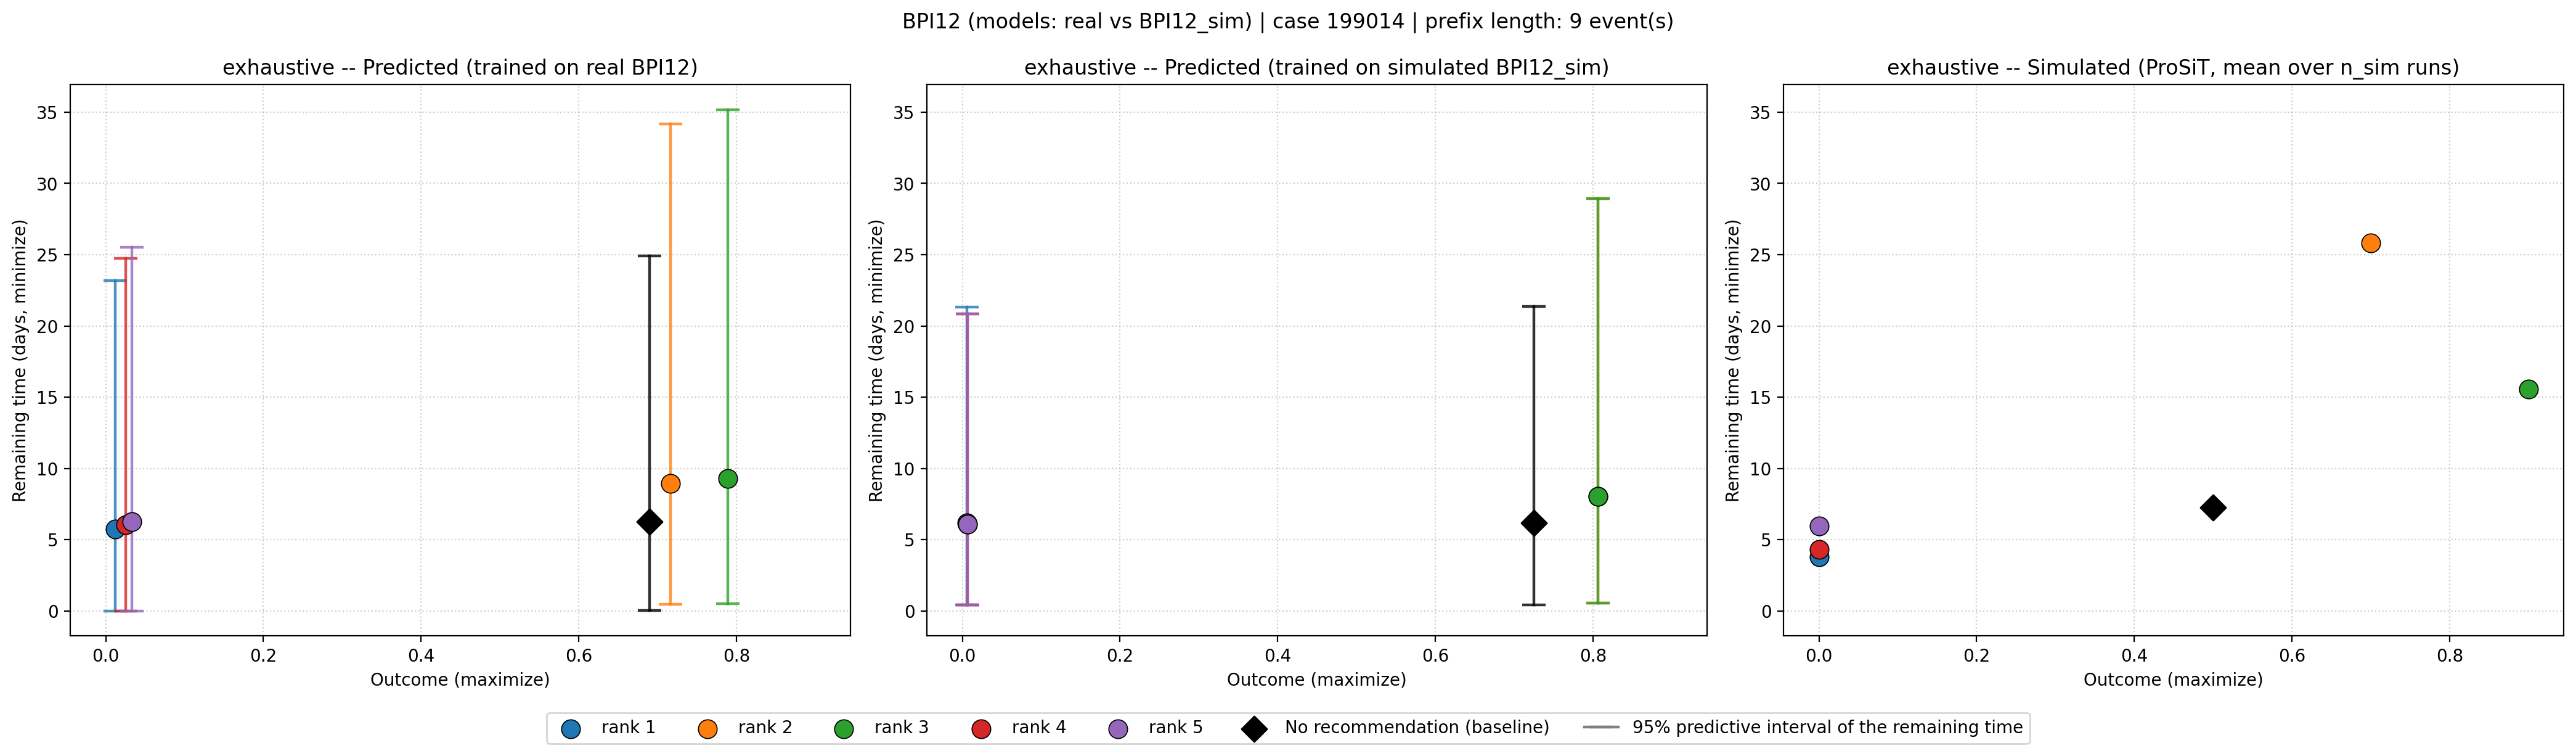
\includegraphics[width=\linewidth]{multi_obj/pareto_fronts/pareto_fronts_bpi12_vs_bpi12sim/BPI12_199014_exhaustive_predicted_vs_simmodel_vs_simulated.png}
\end{frame}

\begin{frame}{BPI12 vs.\ \texttt{BPI12\_sim}: Case 206147 (prefix of 12 events)}
  \centering
  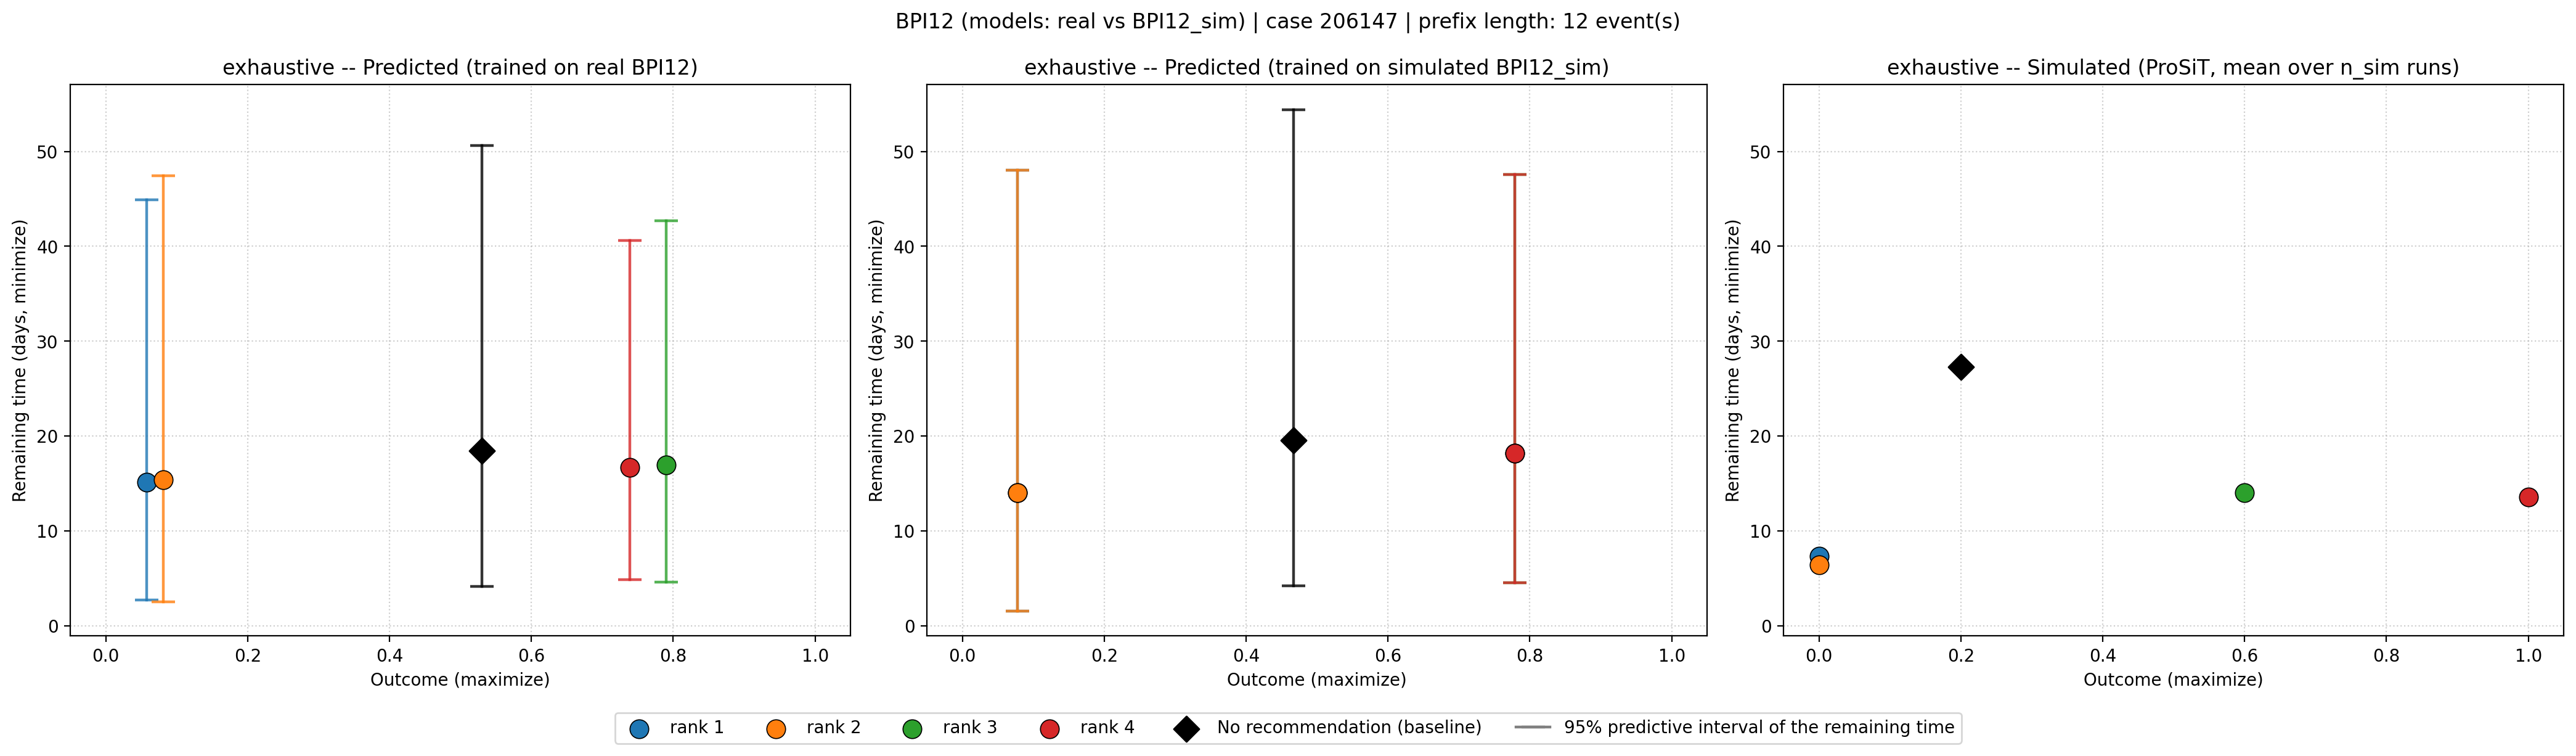
\includegraphics[width=\linewidth]{multi_obj/pareto_fronts/pareto_fronts_bpi12_vs_bpi12sim/BPI12_206147_exhaustive_predicted_vs_simmodel_vs_simulated.png}
\end{frame}

\begin{frame}{BPI12 vs.\ \texttt{BPI12\_sim}: Case 207266 (prefix of 16 events)}
  \centering
  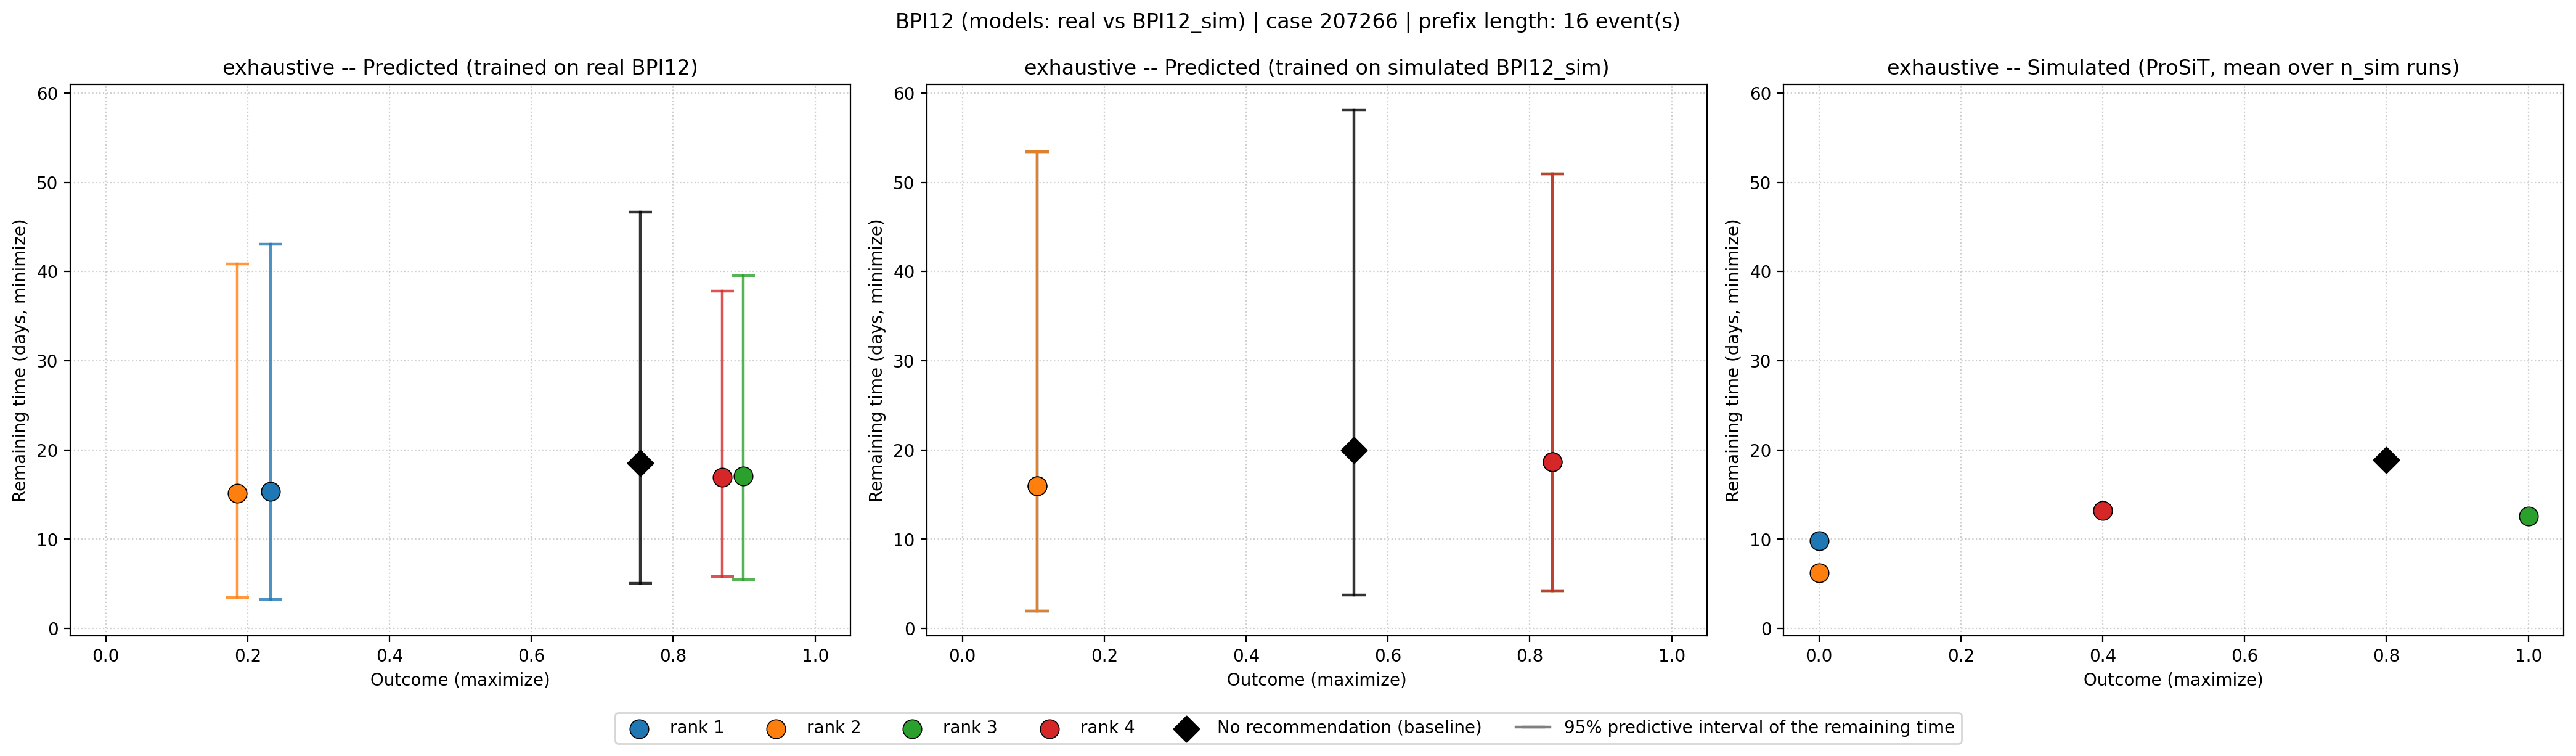
\includegraphics[width=\linewidth]{multi_obj/pareto_fronts/pareto_fronts_bpi12_vs_bpi12sim/BPI12_207266_exhaustive_predicted_vs_simmodel_vs_simulated.png}
\end{frame}

% =====================================================================
% Test without the confidence filter (TEMP_files/test_no_confidence_filter, 2026-10-27)
% =====================================================================
\begin{frame}{Without the Confidence Filter: What the Filter Removes}
  \footnotesize
  Same pipeline with $\gamma_{\text{cls}} = \gamma_{\text{reg}} = -1$ (every candidate passes); baseline,
  simulator and step-9 settings unchanged. \emph{Removed}: points of the unfiltered run that the filter discards.
  \begin{center}\scriptsize\setlength{\tabcolsep}{2pt}
  \begin{tabular}{l c cc cc c cccc}
    \toprule
     & & \multicolumn{2}{c}{Prefixes with rec.} & \multicolumn{2}{c}{Points}
     & & \multicolumn{4}{c}{Removed points: simulated effect} \\
    \cmidrule(lr){3-4}\cmidrule(lr){5-6}\cmidrule(lr){8-11}
    Case study & Prefixes & filter & no filter & filter & no filter & Removed
      & both worse & good & outcome (pp) & time (\%) \\
    \midrule
    BAC          & 1876 & 1871 & 1876 & 2293 & 2298 &  5 (0.2\%) & 20\% & 40\% & $+10.0$ & $+20.9$ \\
    BPI12        &  623 &  601 &  623 &  978 & 1071 & 94 (8.8\%) & 65\% & 10\% & $-51.0$ & $+32.5$ \\
    bpi17-before & 1218 & 1168 & 1218 & 1436 & 1491 & 55 (3.7\%) & 42\% & 33\% & $-3.3$  & $+7.9$  \\
    bpi17-after  & 1840 & 1799 & 1837 & 2345 & 2389 & 47 (2.0\%) & 34\% & 36\% & $-4.5$  & $-5.6$  \\
    \bottomrule
  \end{tabular}
  \end{center}
  \scriptsize
  \begin{itemize}
    \item Removing the filter only \textbf{adds} points: the kept ones are the same as with the filter.
    \item The filter decides \textbf{when not to recommend}: the extra prefixes (+5 / +22 / +50 / +38) have no
      candidate likely to beat ``no recommendation''.
    \item Removed points in the simulation: clearly harmful on BPI12 (65\% worse on both KPIs vs.\ 16\% of the kept
      ones), mildly worse on bpi17; on BAC only 5 points. Time: median change; outcome: mean change.
  \end{itemize}
  {\scriptsize Source: \texttt{multi\_obj/3\_no\_confidence\_filter\_test.txt}.}
\end{frame}

\begin{frame}{Without the Confidence Filter: Effect on the Agreement}
  \footnotesize
  Estimated vs.\ simulated, all points (step 9, $x = 5$, $y = 10$): with the filter / without it.
  Confirmed in \%, discrimination in pp.
  \begin{center}\scriptsize\setlength{\tabcolsep}{2.5pt}
  \begin{tabular}{l cc cc cc cc}
    \toprule
     & \multicolumn{2}{c}{Outcome} & \multicolumn{2}{c}{Remaining time} & \multicolumn{2}{c}{Both KPIs}
     & \multicolumn{2}{c}{Good points} \\
    \cmidrule(lr){2-3}\cmidrule(lr){4-5}\cmidrule(lr){6-7}\cmidrule(lr){8-9}
    Case study & confirmed & discr. & confirmed & discr. & confirmed & discr. & number & good in sim. \\
    \midrule
    BAC          & 54 / 54 & $+3$ / $+6$   & 58 / 58 & $+12$ / $+10$ & 35 / 35 & $+5$ / $+3$   &  508 & 70 / 69 \\
    BPI12        & 81 / 78 & $+81$ / $+76$ & 76 / 77 & $+58$ / $+58$ & 60 / 63 & $+58$ / $+60$ &  501 & 75 / 78 \\
    bpi17-before & 78 / 77 & $+65$ / $+61$ & 77 / 76 & $+35$ / $+30$ & 64 / 63 & $+48$ / $+47$ & 1171 & 80 / 80 \\
    bpi17-after  & 69 / 71 & $+68$ / $+67$ & 70 / 69 & $+29$ / $+26$ & 56 / 57 & $+53$ / $+52$ & 1374 & 80 / 82 \\
    \bottomrule
  \end{tabular}
  \end{center}
  \scriptsize
  \begin{itemize}
    \item All differences within 5 pp: the removed points are estimated not to improve, so they only enter the
      reference group (``estimated no'').
    \item The good points are the same in both variants, simulated in different runs: their confirmation moves by
      up to 3 pp, the noise of 10 runs.
    \item With $\gamma = 0.5$ the filter barely moves the metrics: it withholds recommendations when nothing is
      likely to help and drops clearly harmful actions (BPI12).
  \end{itemize}
  {\scriptsize Source: \texttt{TEMP\_files/test\_no\_confidence\_filter/results/9\_with\_filter.txt},
  \texttt{9\_without\_filter.txt}.}
\end{frame}



\end{document}

